\documentclass[]{article}
\usepackage{lmodern}
\usepackage{amssymb,amsmath}
\usepackage{ifxetex,ifluatex}
\usepackage{fixltx2e} % provides \textsubscript
\ifnum 0\ifxetex 1\fi\ifluatex 1\fi=0 % if pdftex
  \usepackage[T1]{fontenc}
  \usepackage[utf8]{inputenc}
\else % if luatex or xelatex
  \ifxetex
    \usepackage{mathspec}
  \else
    \usepackage{fontspec}
  \fi
  \defaultfontfeatures{Ligatures=TeX,Scale=MatchLowercase}
\fi
% use upquote if available, for straight quotes in verbatim environments
\IfFileExists{upquote.sty}{\usepackage{upquote}}{}
% use microtype if available
\IfFileExists{microtype.sty}{%
\usepackage{microtype}
\UseMicrotypeSet[protrusion]{basicmath} % disable protrusion for tt fonts
}{}
\usepackage[margin=1in]{geometry}
\usepackage{hyperref}
\hypersetup{unicode=true,
            pdftitle={Follow-up on R},
            pdfborder={0 0 0},
            breaklinks=true}
\urlstyle{same}  % don't use monospace font for urls
\usepackage{color}
\usepackage{fancyvrb}
\newcommand{\VerbBar}{|}
\newcommand{\VERB}{\Verb[commandchars=\\\{\}]}
\DefineVerbatimEnvironment{Highlighting}{Verbatim}{commandchars=\\\{\}}
% Add ',fontsize=\small' for more characters per line
\usepackage{framed}
\definecolor{shadecolor}{RGB}{248,248,248}
\newenvironment{Shaded}{\begin{snugshade}}{\end{snugshade}}
\newcommand{\AlertTok}[1]{\textcolor[rgb]{0.94,0.16,0.16}{#1}}
\newcommand{\AnnotationTok}[1]{\textcolor[rgb]{0.56,0.35,0.01}{\textbf{\textit{#1}}}}
\newcommand{\AttributeTok}[1]{\textcolor[rgb]{0.77,0.63,0.00}{#1}}
\newcommand{\BaseNTok}[1]{\textcolor[rgb]{0.00,0.00,0.81}{#1}}
\newcommand{\BuiltInTok}[1]{#1}
\newcommand{\CharTok}[1]{\textcolor[rgb]{0.31,0.60,0.02}{#1}}
\newcommand{\CommentTok}[1]{\textcolor[rgb]{0.56,0.35,0.01}{\textit{#1}}}
\newcommand{\CommentVarTok}[1]{\textcolor[rgb]{0.56,0.35,0.01}{\textbf{\textit{#1}}}}
\newcommand{\ConstantTok}[1]{\textcolor[rgb]{0.00,0.00,0.00}{#1}}
\newcommand{\ControlFlowTok}[1]{\textcolor[rgb]{0.13,0.29,0.53}{\textbf{#1}}}
\newcommand{\DataTypeTok}[1]{\textcolor[rgb]{0.13,0.29,0.53}{#1}}
\newcommand{\DecValTok}[1]{\textcolor[rgb]{0.00,0.00,0.81}{#1}}
\newcommand{\DocumentationTok}[1]{\textcolor[rgb]{0.56,0.35,0.01}{\textbf{\textit{#1}}}}
\newcommand{\ErrorTok}[1]{\textcolor[rgb]{0.64,0.00,0.00}{\textbf{#1}}}
\newcommand{\ExtensionTok}[1]{#1}
\newcommand{\FloatTok}[1]{\textcolor[rgb]{0.00,0.00,0.81}{#1}}
\newcommand{\FunctionTok}[1]{\textcolor[rgb]{0.00,0.00,0.00}{#1}}
\newcommand{\ImportTok}[1]{#1}
\newcommand{\InformationTok}[1]{\textcolor[rgb]{0.56,0.35,0.01}{\textbf{\textit{#1}}}}
\newcommand{\KeywordTok}[1]{\textcolor[rgb]{0.13,0.29,0.53}{\textbf{#1}}}
\newcommand{\NormalTok}[1]{#1}
\newcommand{\OperatorTok}[1]{\textcolor[rgb]{0.81,0.36,0.00}{\textbf{#1}}}
\newcommand{\OtherTok}[1]{\textcolor[rgb]{0.56,0.35,0.01}{#1}}
\newcommand{\PreprocessorTok}[1]{\textcolor[rgb]{0.56,0.35,0.01}{\textit{#1}}}
\newcommand{\RegionMarkerTok}[1]{#1}
\newcommand{\SpecialCharTok}[1]{\textcolor[rgb]{0.00,0.00,0.00}{#1}}
\newcommand{\SpecialStringTok}[1]{\textcolor[rgb]{0.31,0.60,0.02}{#1}}
\newcommand{\StringTok}[1]{\textcolor[rgb]{0.31,0.60,0.02}{#1}}
\newcommand{\VariableTok}[1]{\textcolor[rgb]{0.00,0.00,0.00}{#1}}
\newcommand{\VerbatimStringTok}[1]{\textcolor[rgb]{0.31,0.60,0.02}{#1}}
\newcommand{\WarningTok}[1]{\textcolor[rgb]{0.56,0.35,0.01}{\textbf{\textit{#1}}}}
\usepackage{longtable,booktabs}
\usepackage{graphicx,grffile}
\makeatletter
\def\maxwidth{\ifdim\Gin@nat@width>\linewidth\linewidth\else\Gin@nat@width\fi}
\def\maxheight{\ifdim\Gin@nat@height>\textheight\textheight\else\Gin@nat@height\fi}
\makeatother
% Scale images if necessary, so that they will not overflow the page
% margins by default, and it is still possible to overwrite the defaults
% using explicit options in \includegraphics[width, height, ...]{}
\setkeys{Gin}{width=\maxwidth,height=\maxheight,keepaspectratio}
\IfFileExists{parskip.sty}{%
\usepackage{parskip}
}{% else
\setlength{\parindent}{0pt}
\setlength{\parskip}{6pt plus 2pt minus 1pt}
}
\setlength{\emergencystretch}{3em}  % prevent overfull lines
\providecommand{\tightlist}{%
  \setlength{\itemsep}{0pt}\setlength{\parskip}{0pt}}
\setcounter{secnumdepth}{5}
% Redefines (sub)paragraphs to behave more like sections
\ifx\paragraph\undefined\else
\let\oldparagraph\paragraph
\renewcommand{\paragraph}[1]{\oldparagraph{#1}\mbox{}}
\fi
\ifx\subparagraph\undefined\else
\let\oldsubparagraph\subparagraph
\renewcommand{\subparagraph}[1]{\oldsubparagraph{#1}\mbox{}}
\fi

%%% Use protect on footnotes to avoid problems with footnotes in titles
\let\rmarkdownfootnote\footnote%
\def\footnote{\protect\rmarkdownfootnote}

%%% Change title format to be more compact
\usepackage{titling}

% Create subtitle command for use in maketitle
\providecommand{\subtitle}[1]{
  \posttitle{
    \begin{center}\large#1\end{center}
    }
}

\setlength{\droptitle}{-2em}

  \title{Follow-up on R}
    \pretitle{\vspace{\droptitle}\centering\huge}
  \posttitle{\par}
    \author{}
    \preauthor{}\postauthor{}
    \date{}
    \predate{}\postdate{}
  

\begin{document}
\maketitle

{
\setcounter{tocdepth}{2}
\tableofcontents
}
\hypertarget{about-this-course}{%
\section*{About this course}\label{about-this-course}}
\addcontentsline{toc}{section}{About this course}

\textbf{\emph{Course Content}}

This course builds on introductory R and expands on essential concepts for R. We cover common problems in data manipulation to pre-process datasets and we will cover some visualization. \(99.5\%\) of a data scientist's job is data pre-processing and visualization. The rest is analysis. Therefore, brushing up on programming skills in R makes the experience of working with R a lot more enjoyable.

\textbf{\emph{Course Objectives}}

Participants will learn data manipulation skills such as merging data, re-shaping it, aggregating it and more. Course participants should be a lot more comfortable in working with R upon completing this course.

\textbf{\emph{Course Prerequisites}}

Participants are expected to have used R and RStudio before.

\textbf{\emph{Agenda}}

\begin{enumerate}
\def\labelenumi{\arabic{enumi}.}
\tightlist
\item
  Data sub-setting, logical conditions, missing values, simple plots
\item
  Tidyverse introduction: Simple data manipulation, renaming, summarizing, aggregating
\item
  Merging data, re-shaping data, regular expressions
\end{enumerate}

\textbf{\emph{Acknowledgements}}

The ESRC Business and Local Government Data Research Centre is funded by the \href{https://esrc.ukri.org}{Economic and Social Research Council (ESRC)}.

\begin{center}\rule{0.5\linewidth}{\linethickness}\end{center}

\hypertarget{data-sub-setting-and-logical-conditions}{%
\section{Data sub-setting and logical conditions}\label{data-sub-setting-and-logical-conditions}}

\hypertarget{learning-objectives}{%
\subsection{Learning objectives}\label{learning-objectives}}

In this exercise, we will talk about sub-setting data sets, i.e.~findings interesting observations and variables that we want to describe. Furthermore, we will introduce logical conditions in R. Logical conditions are often necessary for data wrangling.

\hypertarget{sub-setting}{%
\subsubsection{Sub-setting}\label{sub-setting}}

When we deal with data sets and vectors such as data set's rows or columns, we want to be able to subset these objects. Sub-setting means, we access a specific part of the data set or vector. R comes with some small data sets included. The macroeconomic data set \texttt{longley} is one such data set. Lets have a look at what the data set contains by using the help files:

\begin{Shaded}
\begin{Highlighting}[]
\NormalTok{?longley}
\end{Highlighting}
\end{Shaded}

A data set is two-dimensional. It's first dimension are the rows. A 5 on the first dimension, therefore, means row 5. On the second dimension, we have columns. A 4 on the second dimension refers to column 4. We can identify each individual element in a data set by it's row and column coordinates. In R, we subset using square brackets \texttt{{[}\ row.coordinates,\ column.coordinates\ {]}}. In the square brackets, we place the row coordinates first, and column coordinates second. The coordinates are separated by a comma. If we want to see an entire row, we leave the column coordinate unspecified. The first row of the longley data set is:

\begin{Shaded}
\begin{Highlighting}[]
\NormalTok{longley[ }\DecValTok{1}\NormalTok{ , ]}
\end{Highlighting}
\end{Shaded}

\begin{verbatim}
     GNP.deflator     GNP Unemployed Armed.Forces Population Year Employed
1947           83 234.289      235.6          159    107.608 1947   60.323
\end{verbatim}

The second column is:

\begin{Shaded}
\begin{Highlighting}[]
\NormalTok{longley[ , }\DecValTok{2}\NormalTok{ ]}
\end{Highlighting}
\end{Shaded}

\begin{verbatim}
 [1] 234.289 259.426 258.054 284.599 328.975 346.999 365.385 363.112
 [9] 397.469 419.180 442.769 444.546 482.704 502.601 518.173 554.894
\end{verbatim}

The element in the first row and second column is:

\begin{Shaded}
\begin{Highlighting}[]
\NormalTok{longley[ }\DecValTok{1}\NormalTok{ , }\DecValTok{2}\NormalTok{ ]}
\end{Highlighting}
\end{Shaded}

\begin{verbatim}
[1] 234.289
\end{verbatim}

We can view a number of adjacent rows with the colon operator like so:

\begin{Shaded}
\begin{Highlighting}[]
\NormalTok{longley[}\DecValTok{1} \OperatorTok{:}\StringTok{ }\DecValTok{5}\NormalTok{ , ]}
\end{Highlighting}
\end{Shaded}

\begin{verbatim}
     GNP.deflator     GNP Unemployed Armed.Forces Population Year Employed
1947         83.0 234.289      235.6        159.0    107.608 1947   60.323
1948         88.5 259.426      232.5        145.6    108.632 1948   61.122
1949         88.2 258.054      368.2        161.6    109.773 1949   60.171
1950         89.5 284.599      335.1        165.0    110.929 1950   61.187
1951         96.2 328.975      209.9        309.9    112.075 1951   63.221
\end{verbatim}

We can view a number of non adjacent rows using the vector function \texttt{c()} like so:

\begin{Shaded}
\begin{Highlighting}[]
\NormalTok{longley[ }\KeywordTok{c}\NormalTok{(}\DecValTok{1}\NormalTok{,}\DecValTok{3}\NormalTok{,}\DecValTok{5}\NormalTok{), ]}
\end{Highlighting}
\end{Shaded}

\begin{verbatim}
     GNP.deflator     GNP Unemployed Armed.Forces Population Year Employed
1947         83.0 234.289      235.6        159.0    107.608 1947   60.323
1949         88.2 258.054      368.2        161.6    109.773 1949   60.171
1951         96.2 328.975      209.9        309.9    112.075 1951   63.221
\end{verbatim}

Furthermore, columns in data sets have names. These are the variable names. We can obtain a list of variable names with the \texttt{names()} function.

\begin{Shaded}
\begin{Highlighting}[]
\KeywordTok{names}\NormalTok{(longley)}
\end{Highlighting}
\end{Shaded}

\begin{verbatim}
[1] "GNP.deflator" "GNP"          "Unemployed"   "Armed.Forces"
[5] "Population"   "Year"         "Employed"    
\end{verbatim}

This returns a vector of names. You may have noticed the quotation marks. Whenever you see quotation marks in R, you know this refers to a text. There are different storage or data types. Examples are numeric and character (text).

We can use the name of a variable for sub-setting a data set. Suppose, we want to see the population variable. We can either use 5 in square brackets because population is the 5th column or we can place the variable name within quotation marks in the brackets.

\begin{Shaded}
\begin{Highlighting}[]
\NormalTok{longley[ , }\StringTok{"Population"}\NormalTok{]}
\end{Highlighting}
\end{Shaded}

\begin{verbatim}
 [1] 107.608 108.632 109.773 110.929 112.075 113.270 115.094 116.219
 [9] 117.388 118.734 120.445 121.950 123.366 125.368 127.852 130.081
\end{verbatim}

To access multiple variable columns by the variable names, we have to use the vector function \texttt{c()} like so:

\begin{Shaded}
\begin{Highlighting}[]
\NormalTok{longley[ , }\KeywordTok{c}\NormalTok{(}\StringTok{"GNP"}\NormalTok{, }\StringTok{"Armed.Forces"}\NormalTok{, }\StringTok{"Population"}\NormalTok{) ]}
\end{Highlighting}
\end{Shaded}

\begin{verbatim}
         GNP Armed.Forces Population
1947 234.289        159.0    107.608
1948 259.426        145.6    108.632
1949 258.054        161.6    109.773
1950 284.599        165.0    110.929
1951 328.975        309.9    112.075
1952 346.999        359.4    113.270
1953 365.385        354.7    115.094
1954 363.112        335.0    116.219
1955 397.469        304.8    117.388
1956 419.180        285.7    118.734
1957 442.769        279.8    120.445
1958 444.546        263.7    121.950
1959 482.704        255.2    123.366
1960 502.601        251.4    125.368
1961 518.173        257.2    127.852
1962 554.894        282.7    130.081
\end{verbatim}

Finally, we can also access a column in a data set using the dollar sign operator \texttt{\$} like so:

\begin{Shaded}
\begin{Highlighting}[]
\NormalTok{longley}\OperatorTok{$}\NormalTok{Population}
\end{Highlighting}
\end{Shaded}

\begin{verbatim}
 [1] 107.608 108.632 109.773 110.929 112.075 113.270 115.094 116.219
 [9] 117.388 118.734 120.445 121.950 123.366 125.368 127.852 130.081
\end{verbatim}

The population column is a vector. Vectors are 1-dimensional. We can subset vectors in the same way that we subset data sets except that we only need 1 coordinate to uniquely identify every element. Let's access the first element in the population column in three different but equivalent ways.

\begin{Shaded}
\begin{Highlighting}[]
\CommentTok{# option 1s}
\NormalTok{longley}\OperatorTok{$}\NormalTok{Population[}\DecValTok{1}\NormalTok{]}
\end{Highlighting}
\end{Shaded}

\begin{verbatim}
[1] 107.608
\end{verbatim}

\begin{Shaded}
\begin{Highlighting}[]
\CommentTok{# option 2}
\NormalTok{longley[}\DecValTok{1}\NormalTok{ , }\DecValTok{5}\NormalTok{]}
\end{Highlighting}
\end{Shaded}

\begin{verbatim}
[1] 107.608
\end{verbatim}

\begin{Shaded}
\begin{Highlighting}[]
\CommentTok{# option 3}
\NormalTok{longley[}\DecValTok{1}\NormalTok{ , }\StringTok{"Population"}\NormalTok{]}
\end{Highlighting}
\end{Shaded}

\begin{verbatim}
[1] 107.608
\end{verbatim}

Finally, two useful sub-setting tricks:

\begin{enumerate}
\def\labelenumi{\arabic{enumi}.}
\tightlist
\item
  the \texttt{-} operator means except and can be used to view all elements except the one specified
\item
  with the \texttt{length()} function we can find the last element of a vector
\end{enumerate}

So, all rows in the longley data set except the first 5 would be:

\begin{Shaded}
\begin{Highlighting}[]
\NormalTok{longley[ }\DecValTok{-1} \OperatorTok{:}\StringTok{ }\DecValTok{-5}\NormalTok{, ]}
\end{Highlighting}
\end{Shaded}

\begin{verbatim}
     GNP.deflator     GNP Unemployed Armed.Forces Population Year Employed
1952         98.1 346.999      193.2        359.4    113.270 1952   63.639
1953         99.0 365.385      187.0        354.7    115.094 1953   64.989
1954        100.0 363.112      357.8        335.0    116.219 1954   63.761
1955        101.2 397.469      290.4        304.8    117.388 1955   66.019
1956        104.6 419.180      282.2        285.7    118.734 1956   67.857
1957        108.4 442.769      293.6        279.8    120.445 1957   68.169
1958        110.8 444.546      468.1        263.7    121.950 1958   66.513
1959        112.6 482.704      381.3        255.2    123.366 1959   68.655
1960        114.2 502.601      393.1        251.4    125.368 1960   69.564
1961        115.7 518.173      480.6        257.2    127.852 1961   69.331
1962        116.9 554.894      400.7        282.7    130.081 1962   70.551
\end{verbatim}

We can get the length of a vector using the \texttt{length()} function like so:

\begin{Shaded}
\begin{Highlighting}[]
\KeywordTok{length}\NormalTok{( longley[, }\DecValTok{1}\NormalTok{] )}
\end{Highlighting}
\end{Shaded}

\begin{verbatim}
[1] 16
\end{verbatim}

That is the length of the first column in the longley data set and because a data set is rectangular it gives us the number of rows in the data set as well. We get the last row in the longley data set like so:

\begin{Shaded}
\begin{Highlighting}[]
\NormalTok{longley[ }\KeywordTok{length}\NormalTok{( longley[ , }\DecValTok{1}\NormalTok{] ) , ]}
\end{Highlighting}
\end{Shaded}

\begin{verbatim}
     GNP.deflator     GNP Unemployed Armed.Forces Population Year Employed
1962        116.9 554.894      400.7        282.7    130.081 1962   70.551
\end{verbatim}

To get the last element in the population vector of the longley data set, we would code:

\begin{Shaded}
\begin{Highlighting}[]
\NormalTok{longley[ }\KeywordTok{length}\NormalTok{(longley[,}\DecValTok{1}\NormalTok{]), }\StringTok{"Population"}\NormalTok{ ]}
\end{Highlighting}
\end{Shaded}

\begin{verbatim}
[1] 130.081
\end{verbatim}

There are often many different approaches that will do the same thing. In does not matter how you get to a solution as long as get there. For instance, the \texttt{nrow()} function returns the number of rows in a data set or matrix object. So we could get the last element in the population vector using \texttt{nrow()} instead of \texttt{length()}:

\begin{Shaded}
\begin{Highlighting}[]
\NormalTok{longley[ }\KeywordTok{nrow}\NormalTok{(longley), }\StringTok{"Population"}\NormalTok{ ]}
\end{Highlighting}
\end{Shaded}

\begin{verbatim}
[1] 130.081
\end{verbatim}

Sub-setting is essential for understanding data and manipulating it.

Finding the last column of the longley data set can be done using the \texttt{ncol()} function. The function returns the number of columns in the object that is supplied to the function. If we use that number in sub-setting, we can access the last column.

\begin{Shaded}
\begin{Highlighting}[]
\NormalTok{longley[ , }\KeywordTok{ncol}\NormalTok{(longley) ]}
\end{Highlighting}
\end{Shaded}

\begin{verbatim}
 [1] 60.323 61.122 60.171 61.187 63.221 63.639 64.989 63.761 66.019 67.857
[11] 68.169 66.513 68.655 69.564 69.331 70.551
\end{verbatim}

\hypertarget{logical-conditions}{%
\subsubsection{Logical conditions}\label{logical-conditions}}

We now load regional data from the European Union from the \href{http://qog.pol.gu.se/}{Quality of Government Institute} to illustrate logical conditions and dealing with missing values. The data set is very large in the sense that it contains many different columns (variables)

Download Data

A full codebook of the data set is available online (\href{https://www.qogdata.pol.gu.se/data/qog_eureg_sep16.pdf}{codebook})

\begin{Shaded}
\begin{Highlighting}[]
\NormalTok{eu <-}\StringTok{ }\KeywordTok{read.csv}\NormalTok{(}\StringTok{"qog_eureg_long_sep16.csv"}\NormalTok{, }\DataTypeTok{stringsAsFactors =} \OtherTok{FALSE}\NormalTok{)}
\end{Highlighting}
\end{Shaded}

Before, we start working with the data set, do the following tasks on your own:

\begin{enumerate}
\def\labelenumi{\arabic{enumi}.}
\tightlist
\item
  check the dimensions of \texttt{eu}
\item
  check the first 15 variable names of the data set
\item
  print the rows 120 to 130 of the data set and the following variables: ``NUTS0'', ``region\_name'' and econ\_2gdp\_eur\_hab (country name, region name, per capita wealth at current prices)
\end{enumerate}

If you are unsure about a function that you need to complete this task, try looking for it online. For example, googling ``R find names of a data set'' will get you to the function that you need for solving this problem. R does have a steeper learning curve than more traditional data software like Excel. Therefore, it is good practice to get into the habit of searching and learning how to quickly find answers online.

Reveal content

The \texttt{dim()} function returns two numbers. The first is the number of rows and the second is the number of columns (if the object is two-dimensional). The function could also be used on arrays in which case it would also return the number of layers. We could have also found the number of rows using \texttt{nrow()} and the number of columns using \texttt{ncol()}. Or we could have used the \texttt{length()} function with sub-setting. For example, \texttt{length(eu{[},1{]})} returns the length of the first column of the \texttt{u\ which\ is\ equal\ to\ the\ number\ of\ rows\ in\ the\ dataset.\ Equally,}length(eu{[}1,{]})` returns the length of the first row which is equal to the number of columns.

The \texttt{names()} function can be used on several objects such as data frames and lists. Here, \texttt{names()} returns the column names of the data set. In the case that you are dealing with a matrix instead of data frame --- you can assess this by using \texttt{is.data.frame()} and \texttt{is.matrix()} --- you would use the \texttt{colnames()} function for the column names. Here, we have so many variables that \texttt{names()} would fill our screen with a very long vector of variable names. Therefore, we subset the names vector to only display the first 5 variable names

We use \texttt{{[}{]}} for sub-setting. So \texttt{eu{[}1:6,\ 1:4{]}} returns the first six rows and the first four columns of the data set.

\begin{Shaded}
\begin{Highlighting}[]
\CommentTok{# the dimensions: rows (observations) and columns (variables) }
\KeywordTok{dim}\NormalTok{(eu)}
\end{Highlighting}
\end{Shaded}

\begin{verbatim}
[1] 13884   444
\end{verbatim}

\begin{Shaded}
\begin{Highlighting}[]
\CommentTok{# the variable names}
\KeywordTok{names}\NormalTok{(eu)[}\DecValTok{1}\OperatorTok{:}\DecValTok{15}\NormalTok{]}
\end{Highlighting}
\end{Shaded}

\begin{verbatim}
 [1] "region_code"    "region_code_n"  "region_name"    "year"          
 [5] "NUTS_level"     "NUTS0"          "NUTS0_n"        "NUTS1"         
 [9] "NUTS1_n"        "NUTS2"          "NUTS2_n"        "version"       
[13] "demo_cnmigratn" "demo_d2jan_f"   "demo_d2jan_m"  
\end{verbatim}

\begin{Shaded}
\begin{Highlighting}[]
\CommentTok{# top 6 rows of the data}
\NormalTok{eu[}\DecValTok{120}\OperatorTok{:}\DecValTok{130}\NormalTok{, }\KeywordTok{c}\NormalTok{(}\StringTok{"NUTS0"}\NormalTok{, }\StringTok{"region_name"}\NormalTok{, }\StringTok{"econ_2gdp_eur_hab"}\NormalTok{)]}
\end{Highlighting}
\end{Shaded}

\begin{verbatim}
    NUTS0 region_name econ_2gdp_eur_hab
120    AT        Wien             40800
121    AT        Wien             42700
122    AT        Wien             44100
123    AT        Wien             45500
124    AT        Wien             45000
125    AT        Wien             45700
126    AT        Wien             46800
127    AT        Wien             47100
128    AT        Wien             47300
129    AT        Wien             47300
130    AT        Wien                NA
\end{verbatim}

\begin{Shaded}
\begin{Highlighting}[]
\NormalTok{eu}\OperatorTok{$}\NormalTok{econ_2gdp_eur_hab}
\end{Highlighting}
\end{Shaded}

\begin{verbatim}
    [1]     NA     NA     NA     NA     NA     NA     NA     NA     NA
   [10]     NA  26600  27400  28000  28500  29600  30800  32200  34000
   [19]  35100  34300  35200  36800  37600  38100  38500     NA     NA
   [28]     NA     NA     NA     NA     NA     NA     NA     NA     NA
   [37]  28500  29200  29900  30100  31100  32000  33500  35100  36200
   [46]  35600  36300  37600  38100  38500  38700     NA     NA     NA
   [55]     NA     NA     NA     NA     NA     NA     NA     NA  17300
   [64]  17800  18700  19200  20200  20300  21000  22100  22500  22500
   [73]  23400  24300  25500  26100  26500     NA     NA     NA     NA
   [82]     NA     NA     NA     NA     NA     NA     NA  21800  22100
   [91]  22500  23000  24300  24900  26100  27900  28900  28000  28700
  [100]  30100  30700  31200  31400     NA     NA     NA     NA     NA
  [109]     NA     NA     NA     NA     NA     NA  37100  38300  39100
  [118]  38900  39600  40800  42700  44100  45500  45000  45700  46800
  [127]  47100  47300  47300     NA     NA     NA     NA     NA     NA
  [136]     NA     NA     NA     NA     NA  22600  23200  23700  24300
  [145]  25500  26800  27900  29900  30600  29700  30600  32200  33100
  [154]  33300  33900     NA     NA     NA     NA     NA     NA     NA
  [163]     NA     NA     NA     NA  22000  22400  23200  23800  24700
  [172]  25900  27000  28900  29700  28700  29500  31300  31700  31900
  [181]  32200     NA     NA     NA     NA     NA     NA     NA     NA
  [190]     NA     NA     NA  22900  23600  23900  24500  25900  27200
  [199]  28300  30300  31000  30200  31100  32600  33800  33900  34700
  [208]     NA     NA     NA     NA     NA     NA     NA     NA     NA
  [217]     NA     NA  26800  27600  28300  29000  30100  31600  33200
  [226]  35300  36300  35500  36600  38500  39700  40400  41000     NA
  [235]     NA     NA     NA     NA     NA     NA     NA     NA     NA
  [244]     NA  25700  26600  27000  27700  28700  30400  31800  33700
  [253]  35200  34000  35200  37100  38100  38800  39200     NA     NA
  [262]     NA     NA     NA     NA     NA     NA     NA     NA     NA
  [271]  29300  30000  30800  31500  33100  34300  36400  39200  40000
  [280]  39100  41100  43000  44500  44700  45200     NA     NA     NA
  [289]     NA     NA     NA     NA     NA     NA     NA     NA  26800
  [298]  27700  28500  29300  30300  32100  33700  35400  35800  35500
  [307]  36200  37900  39500  40300  41200     NA     NA     NA     NA
  [316]     NA     NA     NA     NA     NA     NA     NA  27200  28300
  [325]  29200  29300  30600  31700  33100  35300  36500  35600  36600
  [334]  38400  39100  40300  41500     NA     NA     NA     NA     NA
  [343]     NA     NA     NA     NA     NA     NA     NA     NA     NA
  [352]     NA     NA     NA     NA     NA     NA     NA     NA     NA
  [361]     NA     NA     NA     NA     NA     NA     NA     NA     NA
  [370]     NA     NA     NA     NA     NA     NA     NA     NA     NA
  [379]     NA     NA     NA     NA     NA     NA     NA     NA     NA
  [388]     NA     NA     NA     NA     NA     NA     NA     NA     NA
  [397]     NA     NA     NA     NA  25200  25900  26600  27200  28700
  [406]  29700  31000  32500  33100  32300  33500  34500  35000  35400
  [415]  35900     NA     NA     NA     NA     NA     NA     NA     NA
  [424]     NA     NA     NA     NA     NA     NA  54100  56600  58700
  [433]  59500  61100  61100  60100  61400  62800  62700  62400  62900
  [442]     NA     NA     NA     NA     NA     NA     NA     NA     NA
  [451]     NA     NA     NA     NA     NA  54100  56600  58700  59500
  [460]  61100  61100  60100  61400  62800  62700  62400  62900     NA
  [469]     NA     NA     NA     NA     NA     NA     NA     NA     NA
  [478]     NA     NA     NA     NA  26900  28400  29500  30900  32600
  [487]  33100  32300  33500  34600  35300  35800  36400     NA     NA
  [496]     NA     NA     NA     NA     NA     NA     NA     NA     NA
  [505]     NA     NA     NA  31700  33700  35600  36700  38600  39200
  [514]  37600  39200  40400  41200  41600  41800     NA     NA     NA
  [523]     NA     NA     NA     NA     NA     NA     NA     NA     NA
  [532]     NA     NA  22800  23500  23800  25300  26700  27400  25900
  [541]  27000  28300  28700  28900  29800     NA     NA     NA     NA
  [550]     NA     NA     NA     NA     NA     NA     NA     NA     NA
  [559]     NA  24000  25400  26100  27300  29000  29400  29300  30300
  [568]  31300  31800  32200  32800     NA     NA     NA     NA     NA
  [577]     NA     NA     NA     NA     NA     NA     NA     NA     NA
  [586]  27800  29400  30600  32400  34000  34500  34700  35300  36200
  [595]  37600  38200  39000     NA     NA     NA     NA     NA     NA
  [604]     NA     NA     NA     NA     NA     NA     NA     NA  25500
  [613]  26800  27600  29300  31000  31200  30500  31700  32800  33500
  [622]  34200  35000     NA     NA     NA     NA     NA     NA     NA
  [631]     NA     NA     NA     NA     NA     NA     NA  19800  20800
  [640]  21500  22500  23500  24400  23700  24900  25400  25500  25700
  [649]  26200     NA     NA     NA     NA     NA     NA     NA     NA
  [658]     NA     NA     NA     NA     NA     NA  27100  29500  30700
  [667]  32100  33800  36200  35000  39800  37200  37300  38300  39500
  [676]     NA     NA     NA     NA     NA     NA     NA     NA     NA
  [685]     NA     NA     NA     NA     NA  18100  18900  19500  20300
  [694]  21100  21900  21000  21700  22700  22800  22900  23100     NA
  [703]     NA     NA     NA     NA     NA     NA     NA     NA     NA
  [712]     NA     NA     NA     NA  19900  21000  21600  22600  23700
  [721]  24400  23800  24400  25600  25800  25900  26200     NA     NA
  [730]     NA     NA     NA     NA     NA     NA     NA     NA     NA
  [739]     NA     NA     NA  18900  19600  20300  21500  21900  22100
  [748]  21500  22200  22800  22700  22800  23200     NA     NA     NA
  [757]     NA     NA     NA     NA     NA     NA     NA     NA     NA
  [766]     NA     NA  19000  19900  20600  21700  22500  23300  23000
  [775]  24000  24400  24600  24700  25200     NA     NA     NA     NA
  [784]     NA     NA     NA     NA     NA     NA     NA     NA     NA
  [793]     NA     NA     NA     NA     NA     NA     NA     NA     NA
  [802]     NA     NA     NA     NA     NA     NA     NA     NA     NA
  [811]     NA     NA     NA     NA     NA     NA     NA     NA     NA
  [820]     NA     NA     NA     NA     NA     NA     NA     NA     NA
  [829]     NA     NA     NA     NA     NA     NA     NA     NA     NA
  [838]     NA     NA     NA     NA     NA   1800   2000   2200   2400
  [847]   2700   3100   3600   4300   4900   4900   5000   5600   5700
  [856]   5800   5900     NA     NA     NA     NA     NA     NA     NA
  [865]     NA     NA     NA     NA     NA     NA     NA     NA     NA
  [874]     NA     NA     NA     NA     NA     NA     NA     NA     NA
  [883]     NA     NA     NA     NA     NA     NA     NA     NA     NA
  [892]     NA     NA     NA     NA     NA     NA     NA     NA     NA
  [901]     NA     NA     NA     NA     NA     NA     NA     NA     NA
  [910]     NA     NA     NA     NA     NA     NA     NA     NA     NA
  [919]     NA     NA     NA     NA     NA     NA     NA     NA     NA
  [928]     NA     NA     NA     NA     NA     NA     NA     NA     NA
  [937]     NA     NA     NA     NA     NA     NA     NA     NA     NA
  [946]     NA     NA     NA     NA     NA     NA     NA     NA     NA
  [955]     NA     NA     NA     NA     NA     NA     NA     NA     NA
  [964]     NA     NA     NA     NA     NA     NA     NA     NA     NA
  [973]     NA     NA     NA     NA     NA     NA     NA     NA     NA
  [982]     NA     NA     NA     NA     NA     NA     NA     NA     NA
  [991]     NA     NA     NA     NA     NA     NA     NA     NA     NA
 [1000]     NA     NA     NA     NA     NA     NA     NA     NA     NA
 [1009]     NA     NA     NA     NA     NA     NA     NA     NA     NA
 [1018]     NA     NA     NA     NA     NA     NA     NA     NA     NA
 [1027]     NA     NA     NA     NA     NA     NA     NA     NA     NA
 [1036]     NA     NA     NA     NA     NA     NA     NA     NA     NA
 [1045]     NA     NA     NA     NA     NA     NA   1600   1800   1900
 [1054]   2100   2300   2600   2800   3300   3700   3700   3700   4100
 [1063]   4300   4400   4600     NA     NA     NA     NA     NA     NA
 [1072]     NA     NA     NA     NA     NA   1500   1700   1900   1900
 [1081]   2100   2300   2500   2900   3200   3100   3100   3500   3600
 [1090]   3600   3800     NA     NA     NA     NA     NA     NA     NA
 [1099]     NA     NA     NA     NA   1400   1700   1900   1900   2100
 [1108]   2400   2600   3000   3400   3300   3300   3800   3900   4100
 [1117]   4300     NA     NA     NA     NA     NA     NA     NA     NA
 [1126]     NA     NA     NA   1700   1800   2000   2100   2400   2700
 [1135]   3100   3700   4200   4000   4100   4500   4700   4800   5000
 [1144]     NA     NA     NA     NA     NA     NA     NA     NA     NA
 [1153]     NA     NA   1800   1900   2000   2200   2500   2900   3100
 [1162]   3500   4000   4100   4100   4500   4800   4900   5000     NA
 [1171]     NA     NA     NA     NA     NA     NA     NA     NA     NA
 [1180]     NA   1900   2200   2500   2800   3200   3700   4300   5400
 [1189]   6200   6300   6500   7100   7200   7200   7300     NA     NA
 [1198]     NA     NA     NA     NA     NA     NA     NA     NA     NA
 [1207]   2400   2800   3200   3500   4000   4600   5600   7000   8200
 [1216]   8300   8600   9300   9300   9300   9500     NA     NA     NA
 [1225]     NA     NA     NA     NA     NA     NA     NA     NA   1300
 [1234]   1500   1600   1800   2100   2400   2700   3100   3400   3400
 [1243]   3500   3900   4000   4100   4000     NA     NA     NA     NA
 [1252]     NA     NA     NA     NA     NA     NA     NA     NA     NA
 [1261]     NA     NA     NA     NA     NA     NA     NA     NA     NA
 [1270]     NA     NA     NA     NA     NA     NA     NA     NA     NA
 [1279]     NA     NA     NA     NA     NA     NA     NA     NA     NA
 [1288]     NA     NA     NA     NA     NA     NA     NA     NA     NA
 [1297]     NA     NA     NA     NA     NA     NA     NA     NA     NA
 [1306]     NA     NA     NA     NA     NA  15500  16400  16900  17800
 [1315]  19000  20200  21500  22800  23900  22900  23100  23000  22500
 [1324]  21000  20400     NA     NA     NA     NA     NA     NA     NA
 [1333]     NA     NA     NA     NA  15500  16400  16900  17800  19000
 [1342]  20200  21500  22800  23900  22900  23100  23000  22500  21000
 [1351]  20400     NA     NA     NA     NA     NA     NA     NA     NA
 [1360]     NA     NA     NA  15500  16400  16900  17800  19000  20200
 [1369]  21500  22800  23900  22900  23100  23000  22500  21000  20400
 [1378]     NA     NA     NA     NA     NA     NA     NA     NA     NA
 [1387]     NA     NA     NA     NA     NA     NA     NA     NA     NA
 [1396]     NA     NA     NA     NA     NA     NA     NA     NA     NA
 [1405]     NA     NA     NA     NA     NA     NA     NA     NA     NA
 [1414]     NA     NA     NA     NA     NA     NA     NA     NA     NA
 [1423]     NA     NA     NA     NA     NA     NA     NA     NA     NA
 [1432]     NA     NA     NA     NA     NA     NA     NA     NA     NA
 [1441]   6500   7400   8500   8600   9400  10700  12100  13400  15400
 [1450]  14100  14900  15600  15300  14900  14700     NA     NA     NA
 [1459]     NA     NA     NA     NA     NA     NA     NA     NA   6500
 [1468]   7400   8500   8600   9400  10700  12100  13400  15400  14100
 [1477]  14900  15600  15300  14900  14700     NA     NA     NA     NA
 [1486]     NA     NA     NA     NA     NA     NA     NA  12800  14900
 [1495]  17500  18200  19800  22800  25800  29100  33600  30500  32100
 [1504]  32900  31900  31100  30100     NA     NA     NA     NA     NA
 [1513]     NA     NA     NA     NA     NA     NA   6500   7300   8500
 [1522]   8300   9000   9900  11400  12600  14500  12800  13200  14100
 [1531]  13800  13400  13400     NA     NA     NA     NA     NA     NA
 [1540]     NA     NA     NA     NA     NA   6100   6800   7900   7900
 [1549]   8700   9800  11100  11800  13100  12400  13100  13700  13300
 [1558]  13300  13200     NA     NA     NA     NA     NA     NA     NA
 [1567]     NA     NA     NA     NA   5400   6000   7000   7100   7600
 [1576]   8600   9500  10400  11900  11300  11500  11900  11700  11300
 [1585]  10900     NA     NA     NA     NA     NA     NA     NA     NA
 [1594]     NA     NA     NA   5800   6500   7400   7300   7900   9000
 [1603]  10000  11000  12500  11500  12200  12900  12400  12200  12100
 [1612]     NA     NA     NA     NA     NA     NA     NA     NA     NA
 [1621]     NA     NA   5700   6500   7500   7700   8200   9300  10500
 [1630]  11800  13800  12700  13300  14100  14200  14100  13700     NA
 [1639]     NA     NA     NA     NA     NA     NA     NA     NA     NA
 [1648]     NA   5200   5900   6700   6800   7400   8300   9300  10300
 [1657]  12200  11200  11800  12600  12400  12100  12200     NA     NA
 [1666]     NA     NA     NA     NA     NA     NA     NA     NA     NA
 [1675]   5000   5700   6500   6600   7600   9000   9900  11000  12900
 [1684]  11500  12300  13300  13200  12400  12300     NA     NA     NA
 [1693]     NA     NA     NA     NA     NA     NA     NA     NA     NA
 [1702]     NA     NA     NA     NA     NA     NA     NA     NA     NA
 [1711]     NA     NA     NA     NA     NA     NA     NA     NA     NA
 [1720]     NA     NA     NA     NA     NA     NA     NA     NA     NA
 [1729]     NA     NA     NA     NA     NA     NA     NA     NA     NA
 [1738]     NA     NA     NA     NA     NA     NA     NA     NA     NA
 [1747]     NA     NA     NA     NA     NA     NA  26000  26700  27100
 [1756]  27200  27900  28300  29500  31000  31700  30600  32100  33700
 [1765]  34300  35000  36000     NA     NA     NA     NA     NA     NA
 [1774]     NA     NA     NA     NA     NA  29700  30900  31000  31100
 [1783]  31400  31700  33700  35600  36000  33600  36400  38700  39200
 [1792]  39900  41200     NA     NA     NA     NA     NA     NA     NA
 [1801]     NA     NA     NA     NA  33300  35000  34800  35200  35200
 [1810]  35100  37700  40200  39800  36600  40500  43000  43900  44700
 [1819]  46300     NA     NA     NA     NA     NA     NA     NA     NA
 [1828]     NA     NA     NA  29600  30600  31000  31000  31500  32200
 [1837]  33900  35400  36300  34500  36500  38500  38700  39000  40200
 [1846]     NA     NA     NA     NA     NA     NA     NA     NA     NA
 [1855]     NA     NA  25600  26200  26300  26300  26700  27100  28500
 [1864]  29800  30600  28900  30800  32800  33100  33900  35000     NA
 [1873]     NA     NA     NA     NA     NA     NA     NA     NA     NA
 [1882]     NA  27000  27900  28000  28100  28800  29300  30800  32700
 [1891]  33700  31300  34100  36500  36800  37600  38900     NA     NA
 [1900]     NA     NA     NA     NA     NA     NA     NA     NA     NA
 [1909]  29700  30600  31200  30900  31800  32300  33600  35200  35500
 [1918]  34700  36600  38600  39400  40300  41400     NA     NA     NA
 [1927]     NA     NA     NA     NA     NA     NA     NA     NA  38600
 [1936]  40000  40400  39800  40900  41500  42900  45000  44300  43300
 [1945]  45100  47700  48600  50000  51200     NA     NA     NA     NA
 [1954]     NA     NA     NA     NA     NA     NA     NA  23400  24800
 [1963]  25200  24900  26000  26400  27300  28900  29400  28800  31300
 [1972]  33100  33100  33900  34800     NA     NA     NA     NA     NA
 [1981]     NA     NA     NA     NA     NA     NA  24800  25100  25800
 [1990]  25800  26400  27200  28200  30100  31200  30300  32600  34300
 [1999]  35000  35600  36700     NA     NA     NA     NA     NA     NA
 [2008]     NA     NA     NA     NA     NA  22900  23800  23800  23500
 [2017]  24300  24400  26000  27000  27400  27600  29000  30300  31000
 [2026]  31500  32700     NA     NA     NA     NA     NA     NA     NA
 [2035]     NA     NA     NA     NA  28300  28200  29200  29000  30300
 [2044]  30100  31100  32500  33500  33100  34600  36300  37200  37600
 [2053]  38800     NA     NA     NA     NA     NA     NA     NA     NA
 [2062]     NA     NA     NA  25200  26300  26800  26800  27300  28200
 [2071]  29200  30600  31000  29800  31800  34000  34600  35100  36300
 [2080]     NA     NA     NA     NA     NA     NA     NA     NA     NA
 [2089]     NA     NA  25200  26100  27000  26500  27200  27700  29100
 [2098]  30000  30900  30000  31700  33200  34100  34900  35800     NA
 [2107]     NA     NA     NA     NA     NA     NA     NA     NA     NA
 [2116]     NA  25400  25700  25700  25500  25500  26000  26900  28200
 [2125]  29400  29400  30500  32800  32700  33200  34200     NA     NA
 [2134]     NA     NA     NA     NA     NA     NA     NA     NA     NA
 [2143]  25400  25700  25700  25500  25500  26000  26900  28200  29400
 [2152]  29400  30500  32800  32700  33200  34200     NA     NA     NA
 [2161]     NA     NA     NA     NA     NA     NA     NA     NA  17400
 [2170]  17800  18200  18400  18900  19300  20200  21200  22100  21700
 [2179]  22800  23500  24100  24700  25300     NA     NA     NA     NA
 [2188]     NA     NA     NA     NA     NA     NA     NA  17400  17800
 [2197]  18200  18400  18900  19300  20200  21200  22100  21700  22800
 [2206]  23500  24100  24700  25300     NA     NA     NA     NA     NA
 [2215]     NA     NA     NA     NA     NA     NA     NA     NA     NA
 [2224]     NA     NA     NA     NA     NA     NA     NA     NA     NA
 [2233]     NA     NA     NA     NA     NA     NA     NA     NA     NA
 [2242]     NA     NA     NA     NA     NA     NA     NA     NA     NA
 [2251]     NA     NA     NA     NA     NA     NA     NA     NA     NA
 [2260]     NA     NA     NA     NA     NA     NA     NA     NA     NA
 [2269]     NA     NA     NA     NA  34100  35400  36500  37300  37700
 [2278]  38300  40100  41700  42500  38900  41500  42700  44500  45000
 [2287]  46000     NA     NA     NA     NA     NA     NA     NA     NA
 [2296]     NA     NA     NA  34100  35400  36500  37300  37700  38300
 [2305]  40100  41700  42500  38900  41500  42700  44500  45000  46000
 [2314]     NA     NA     NA     NA     NA     NA     NA     NA     NA
 [2323]     NA     NA  45900  48300  49000  49100  50100  51200  51700
 [2332]  53200  54600  52300  54200  56100  56600  57400  59000     NA
 [2341]     NA     NA     NA     NA     NA     NA     NA     NA     NA
 [2350]     NA  45900  48300  49000  49100  50100  51200  51700  53200
 [2359]  54600  52300  54200  56100  56600  57400  59000     NA     NA
 [2368]     NA     NA     NA     NA     NA     NA     NA     NA     NA
 [2377]  32400  33500  33700  34500  35000  35300  36500  38100  38600
 [2386]  36800  38200  39400  39500  40400  41400     NA     NA     NA
 [2395]     NA     NA     NA     NA     NA     NA     NA     NA  37700
 [2404]  39100  39000  40000  40500  40700  42100  43700  44200  42100
 [2413]  43400  44800  44700  45500  46600     NA     NA     NA     NA
 [2422]     NA     NA     NA     NA     NA     NA     NA  23500  24100
 [2431]  24400  24700  25500  25900  26700  28300  29200  27200  28300
 [2440]  29300  29500  30300  31200     NA     NA     NA     NA     NA
 [2449]     NA     NA     NA     NA     NA     NA  24400  25100  25700
 [2458]  26600  26800  26900  28100  29300  29700  28700  30300  31000
 [2467]  31500  32700  33800     NA     NA     NA     NA     NA     NA
 [2476]     NA     NA     NA     NA     NA  16700  17100  17500  17800
 [2485]  18200  18400  19100  20300  21100  21100  21800  22600  22900
 [2494]  23400  24200     NA     NA     NA     NA     NA     NA     NA
 [2503]     NA     NA     NA     NA  16700  17100  17500  17800  18200
 [2512]  18400  19100  20300  21100  21100  21800  22600  22900  23400
 [2521]  24200     NA     NA     NA     NA     NA     NA     NA     NA
 [2530]     NA     NA     NA  23500  23800  23600  23700  24300  24900
 [2539]  26000  27200  28100  26900  28700  30300  31000  31800  32600
 [2548]     NA     NA     NA     NA     NA     NA     NA     NA     NA
 [2557]     NA     NA  25900  26600  25700  26100  26900  27700  28700
 [2566]  30600  30900  28800  32100  35000  35700  37900  39100     NA
 [2575]     NA     NA     NA     NA     NA     NA     NA     NA     NA
 [2584]     NA  25800  26000  26300  26300  26600  27800  29200  29800
 [2593]  30800  29700  31100  32900  33300  33900  34700     NA     NA
 [2602]     NA     NA     NA     NA     NA     NA     NA     NA     NA
 [2611]  18900  19000  19000  19000  19400  19500  20300  21400  22000
 [2620]  21600  22400  23300  24200  24700  25200     NA     NA     NA
 [2629]     NA     NA     NA     NA     NA     NA     NA     NA  22900
 [2638]  23400  23100  23100  24000  24100  25300  26700  28000  27000
 [2647]  28600  29900  30500  30900  31700     NA     NA     NA     NA
 [2656]     NA     NA     NA     NA     NA     NA     NA  26200  26800
 [2665]  27300  27300  28100  28500  29500  31400  32300  31200  32300
 [2674]  33600  34100  34600  35600     NA     NA     NA     NA     NA
 [2683]     NA     NA     NA     NA     NA     NA  28100  29200  29600
 [2692]  29900  30800  31200  32000  34300  35900  34400  35100  36300
 [2701]  36900  37400  38500     NA     NA     NA     NA     NA     NA
 [2710]     NA     NA     NA     NA     NA  29400  29800  30900  30200
 [2719]  30800  30800  32100  34000  34200  33800  34700  36000  36200
 [2728]  36900  37900     NA     NA     NA     NA     NA     NA     NA
 [2737]     NA     NA     NA     NA  22400  22900  23000  23300  24300
 [2746]  24800  25900  27400  28500  27200  28500  29400  29900  30300
 [2755]  31200     NA     NA     NA     NA     NA     NA     NA     NA
 [2764]     NA     NA     NA  25900  26100  26200  26200  26700  27500
 [2773]  28400  30500  31000  29900  30900  32400  33200  34000  34900
 [2782]     NA     NA     NA     NA     NA     NA     NA     NA     NA
 [2791]     NA     NA  23000  23200  23500  23800  24500  25200  26200
 [2800]  27700  28600  27400  28900  30500  30900  31400  32300     NA
 [2809]     NA     NA     NA     NA     NA     NA     NA     NA     NA
 [2818]     NA  23600  23700  24200  24300  25100  25200  26300  27500
 [2827]  28100  27500  29100  30100  30700  31200  32000     NA     NA
 [2836]     NA     NA     NA     NA     NA     NA     NA     NA     NA
 [2845]  22400  22500  23100  23200  23900  24200  25300  26300  26900
 [2854]  26300  27900  28600  29200  29700  30500     NA     NA     NA
 [2863]     NA     NA     NA     NA     NA     NA     NA     NA  20500
 [2872]  20800  21400  21900  22600  22700  23400  24300  25000  24500
 [2881]  25400  26200  26600  27700  28400     NA     NA     NA     NA
 [2890]     NA     NA     NA     NA     NA     NA     NA  25400  25300
 [2899]  25700  25700  26600  26700  27700  29200  29700  29200  31000
 [2908]  32100  33000  33300  34000     NA     NA     NA     NA     NA
 [2917]     NA     NA     NA     NA     NA     NA  24000  24600  24700
 [2926]  25000  26200  27600  28900  30600  31200  28400  30300  32100
 [2935]  32600  32900  34000     NA     NA     NA     NA     NA     NA
 [2944]     NA     NA     NA     NA     NA  24000  24600  24700  25000
 [2953]  26200  27600  28900  30600  31200  28400  30300  32100  32600
 [2962]  32900  34000     NA     NA     NA     NA     NA     NA     NA
 [2971]     NA     NA     NA     NA  17200  17900  18800  19300  20000
 [2980]  20100  21200  22300  22800  22200  23300  24500  25100  26000
 [2989]  26900     NA     NA     NA     NA     NA     NA     NA     NA
 [2998]     NA     NA     NA     NA     NA     NA     NA     NA     NA
 [3007]     NA     NA     NA     NA     NA     NA     NA     NA     NA
 [3016]     NA     NA     NA     NA     NA     NA     NA     NA     NA
 [3025]     NA     NA  17500  18400  19500  20200  21000  21000  21800
 [3034]  23000  23200  22700  23600  24500  25100  26200  27100     NA
 [3043]     NA     NA     NA     NA     NA     NA     NA     NA     NA
 [3052]     NA     NA     NA     NA     NA     NA     NA     NA     NA
 [3061]     NA     NA     NA     NA     NA     NA     NA     NA     NA
 [3070]     NA     NA     NA     NA     NA     NA     NA     NA     NA
 [3079]  16200  16700  17400  17900  18500  18700  20000  21100  21600
 [3088]  20800  22100  23100  23500  24000  25100     NA     NA     NA
 [3097]     NA     NA     NA     NA     NA     NA     NA     NA  18500
 [3106]  19100  19900  20200  20700  20800  22200  23300  23900  23700
 [3115]  24700  26600  27500  28700  29400     NA     NA     NA     NA
 [3124]     NA     NA     NA     NA     NA     NA     NA  16300  16800
 [3133]  17600  18000  18500  18800  19800  21000  21600  20900  22400
 [3142]  22800  23800  24400  24900     NA     NA     NA     NA     NA
 [3151]     NA     NA     NA     NA     NA     NA  16300  16800  17600
 [3160]  18000  18500  18800  19800  21000  21600  20900  22400  22800
 [3169]  23800  24400  24900     NA     NA     NA     NA     NA     NA
 [3178]     NA     NA     NA     NA     NA     NA     NA     NA     NA
 [3187]     NA     NA     NA     NA     NA     NA     NA     NA     NA
 [3196]     NA     NA     NA     NA     NA     NA     NA     NA     NA
 [3205]     NA     NA     NA     NA     NA     NA     NA     NA     NA
 [3214]     NA     NA     NA     NA     NA     NA     NA     NA     NA
 [3223]     NA     NA     NA     NA     NA     NA     NA     NA     NA
 [3232]     NA     NA     NA     NA     NA     NA     NA     NA     NA
 [3241]     NA     NA     NA     NA     NA     NA     NA     NA     NA
 [3250]     NA     NA     NA     NA     NA     NA     NA     NA     NA
 [3259]     NA     NA  23300  23900  23600  23800  24300  24400  25200
 [3268]  25900  26700  26000  26600  27400  28500  29000  29900     NA
 [3277]     NA     NA     NA     NA     NA     NA     NA     NA     NA
 [3286]     NA  23300  23900  23600  23800  24300  24400  25200  25900
 [3295]  26700  26000  26600  27400  28500  29000  29900     NA     NA
 [3304]     NA     NA     NA     NA     NA     NA     NA     NA     NA
 [3313]  16400  17000  17400  17900  18500  18700  19600  20700  21200
 [3322]  20500  21900  23300  23800  24400  25300     NA     NA     NA
 [3331]     NA     NA     NA     NA     NA     NA     NA     NA  16400
 [3340]  17000  17400  17900  18500  18700  19600  20700  21200  20500
 [3349]  21900  23300  23800  24400  25300     NA     NA     NA     NA
 [3358]     NA     NA     NA     NA     NA     NA     NA     NA     NA
 [3367]     NA     NA     NA     NA     NA     NA     NA     NA     NA
 [3376]     NA     NA     NA     NA     NA     NA     NA     NA     NA
 [3385]     NA     NA     NA     NA     NA     NA     NA     NA     NA
 [3394]     NA     NA     NA     NA     NA     NA     NA     NA     NA
 [3403]     NA     NA     NA     NA     NA     NA     NA     NA     NA
 [3412]     NA     NA     NA     NA     NA  33300  34400  35300  35900
 [3421]  37400  39300  41500  42800  43900  41700  43500  44200  45200
 [3430]  45500  46200     NA     NA     NA     NA     NA     NA     NA
 [3439]     NA     NA     NA     NA  32300  33500  34400  35000  36300
 [3448]  37700  39800  41000  42000  40500  42100  42600  43600  44100
 [3457]  45000     NA     NA     NA     NA     NA     NA     NA     NA
 [3466]     NA     NA     NA     NA     NA     NA     NA     NA     NA
 [3475]     NA     NA     NA     NA     NA     NA     NA     NA     NA
 [3484]     NA     NA     NA     NA     NA     NA     NA     NA     NA
 [3493]     NA     NA  40100  41300  41800  42800  45300  48600  49700
 [3502]  51300  53100  51300  54900  54400  56100  56600  58100     NA
 [3511]     NA     NA     NA     NA     NA     NA     NA     NA     NA
 [3520]     NA  23900  25000  25900  26300  27400  28200  29700  30100
 [3529]  29600  28700  30000  30100  31100  30900  31600     NA     NA
 [3538]     NA     NA     NA     NA     NA     NA     NA     NA     NA
 [3547]  30000  31000  32000  32600  33500  33900  36500  38100  39000
 [3556]  37000  38400  39200  40000  40700  41300     NA     NA     NA
 [3565]     NA     NA     NA     NA     NA     NA     NA     NA  31100
 [3574]  32400  33600  33700  34700  35200  38200  39200  40200  38900
 [3583]  38800  40200  40500  40900  41300     NA     NA     NA     NA
 [3592]     NA     NA     NA     NA     NA     NA     NA  29200  30200
 [3601]  31800  32300  32500  33300  35800  37000  38000  36700  37200
 [3610]  37500  38700  39000  39600     NA     NA     NA     NA     NA
 [3619]     NA     NA     NA     NA     NA     NA     NA     NA     NA
 [3628]     NA     NA     NA     NA     NA     NA     NA     NA     NA
 [3637]     NA     NA     NA     NA     NA     NA     NA     NA     NA
 [3646]     NA     NA     NA     NA     NA     NA     NA     NA     NA
 [3655]     NA     NA     NA     NA     NA     NA     NA     NA     NA
 [3664]     NA     NA     NA     NA     NA     NA     NA     NA     NA
 [3673]     NA     NA     NA     NA   4400   5000   5600   6300   7100
 [3682]   8300  10000  12100  12300  10600  11000  12500  13600  14400
 [3691]  15200     NA     NA     NA     NA     NA     NA     NA     NA
 [3700]     NA     NA     NA   4400   5000   5600   6300   7100   8300
 [3709]  10000  12100  12300  10600  11000  12500  13600  14400  15200
 [3718]     NA     NA     NA     NA     NA     NA     NA     NA     NA
 [3727]     NA     NA   4400   5000   5600   6300   7100   8300  10000
 [3736]  12100  12300  10600  11000  12500  13600  14400  15200     NA
 [3745]     NA     NA     NA     NA     NA     NA     NA     NA     NA
 [3754]     NA     NA     NA     NA     NA     NA     NA     NA     NA
 [3763]     NA     NA     NA     NA     NA     NA     NA     NA     NA
 [3772]     NA     NA     NA     NA     NA     NA     NA     NA     NA
 [3781]     NA     NA     NA     NA     NA     NA     NA     NA     NA
 [3790]     NA     NA     NA     NA     NA     NA     NA     NA     NA
 [3799]     NA     NA     NA     NA     NA     NA     NA     NA  13200
 [3808]  14000  15000  16400  17700  18100  19800  21100  21800  21400
 [3817]  20300  18600  17300  16500  16200     NA     NA     NA     NA
 [3826]     NA     NA     NA     NA     NA     NA     NA     NA     NA
 [3835]     NA     NA     NA     NA     NA     NA     NA     NA     NA
 [3844]     NA     NA     NA     NA     NA     NA     NA     NA     NA
 [3853]     NA     NA     NA     NA     NA     NA     NA     NA     NA
 [3862]     NA     NA     NA     NA     NA     NA     NA     NA     NA
 [3871]     NA     NA     NA     NA     NA     NA     NA     NA     NA
 [3880]     NA     NA     NA     NA     NA     NA     NA     NA     NA
 [3889]     NA     NA     NA     NA     NA     NA     NA     NA     NA
 [3898]     NA     NA     NA     NA     NA     NA     NA     NA     NA
 [3907]     NA     NA     NA     NA     NA     NA     NA     NA     NA
 [3916]     NA     NA     NA     NA     NA     NA     NA     NA     NA
 [3925]     NA     NA     NA     NA     NA     NA     NA     NA     NA
 [3934]     NA     NA     NA     NA     NA     NA     NA     NA     NA
 [3943]     NA     NA     NA     NA     NA     NA     NA     NA     NA
 [3952]     NA     NA     NA     NA     NA     NA     NA     NA     NA
 [3961]     NA     NA     NA     NA     NA     NA     NA     NA     NA
 [3970]     NA     NA     NA     NA     NA     NA     NA     NA     NA
 [3979]     NA     NA     NA     NA     NA     NA     NA     NA     NA
 [3988]     NA     NA     NA     NA     NA     NA     NA     NA     NA
 [3997]     NA     NA     NA     NA     NA     NA     NA     NA     NA
 [4006]     NA     NA     NA     NA     NA     NA     NA     NA     NA
 [4015]     NA     NA     NA     NA     NA     NA     NA     NA     NA
 [4024]     NA     NA     NA     NA     NA     NA     NA     NA     NA
 [4033]     NA     NA     NA     NA     NA     NA     NA     NA     NA
 [4042]     NA     NA     NA     NA     NA     NA     NA     NA     NA
 [4051]     NA     NA     NA     NA     NA     NA     NA     NA     NA
 [4060]     NA     NA     NA     NA     NA     NA     NA     NA     NA
 [4069]     NA     NA     NA     NA     NA     NA     NA     NA     NA
 [4078]     NA     NA     NA     NA     NA     NA     NA     NA     NA
 [4087]     NA     NA     NA     NA     NA     NA     NA     NA     NA
 [4096]     NA     NA     NA     NA     NA     NA     NA     NA     NA
 [4105]     NA     NA     NA     NA     NA     NA     NA     NA     NA
 [4114]     NA     NA     NA     NA     NA  16700  17700  19300  21000
 [4123]  23000  23700  26200  28100  29200  29000  27600  25400  23500
 [4132]  22200  22200     NA     NA     NA     NA     NA     NA     NA
 [4141]     NA     NA     NA     NA  16700  17700  19300  21000  23000
 [4150]  23700  26200  28100  29200  29000  27600  25400  23500  22200
 [4159]  22200     NA     NA     NA     NA     NA     NA     NA     NA
 [4168]     NA     NA     NA  12700  13400  13900  15400  16700  17200
 [4177]  18500  19500  20500  19500  18400  16600  15100  14800  15000
 [4186]     NA     NA     NA     NA     NA     NA     NA     NA     NA
 [4195]     NA     NA   9800  10300  10600  12500  13200  14000  15300
 [4204]  16700  17600  17000  15900  14700  13400  12900  12800     NA
 [4213]     NA     NA     NA     NA     NA     NA     NA     NA     NA
 [4222]     NA  15700  16200  16300  18200  19700  20600  22000  23400
 [4231]  24700  22900  21700  19700  18200  17400  18000     NA     NA
 [4240]     NA     NA     NA     NA     NA     NA     NA     NA     NA
 [4249]  12100  12900  13700  14800  16200  16400  17600  18300  19200
 [4258]  18500  17400  15500  14000  14000  14100     NA     NA     NA
 [4267]     NA     NA     NA     NA     NA     NA     NA     NA  10700
 [4276]  11400  12100  13100  14000  14100  15200  16200  16700  16400
 [4285]  15600  14400  13400  12700  12400     NA     NA     NA     NA
 [4294]     NA     NA     NA     NA     NA     NA     NA  10200  10700
 [4303]  11300  12100  12800  13100  13500  14700  15600  15300  15100
 [4312]  13300  12400  11500  11200     NA     NA     NA     NA     NA
 [4321]     NA     NA     NA     NA     NA     NA  10900  11600  12200
 [4330]  13100  14200  14300  15600  16800  17400  16900  15800  14600
 [4339]  13500  12800  12500     NA     NA     NA     NA     NA     NA
 [4348]     NA     NA     NA     NA     NA  11500  12300  13500  15000
 [4357]  15900  16600  17200  17400  16700  17600  17400  16900  16700
 [4366]  15700  14800     NA     NA     NA     NA     NA     NA     NA
 [4375]     NA     NA     NA     NA  10100  10700  11600  12600  12900
 [4384]  13200  13900  14600  15000  14500  14200  13300  12200  11600
 [4393]  11400     NA     NA     NA     NA     NA     NA     NA     NA
 [4402]     NA     NA     NA  11300  12000  12600  13900  14700  15000
 [4411]  16200  17100  17600  16900  16000  14700  13900  13300  12900
 [4420]     NA     NA     NA     NA     NA     NA     NA     NA     NA
 [4429]     NA     NA  10200  10900  11700  13300  14000  13800  15100
 [4438]  15800  16400  15800  14500  13300  12800  12600  12300     NA
 [4447]     NA     NA     NA     NA     NA     NA     NA     NA     NA
 [4456]     NA  13300  14200  14300  16400  17500  18300  19500  20700
 [4465]  21800  20200  19100  16600  15600  14700  15100     NA     NA
 [4474]     NA     NA     NA     NA     NA     NA     NA     NA     NA
 [4483]   9900  10500  11400  12500  13600  14000  15400  16200  16400
 [4492]  15700  15400  13900  13100  12200  12100     NA     NA     NA
 [4501]     NA     NA     NA     NA     NA     NA     NA     NA  14100
 [4510]  14800  15200  16400  16900  17500  18200  19000  19600  18600
 [4519]  17700  16500  15400  14900  13800     NA     NA     NA     NA
 [4528]     NA     NA     NA     NA     NA     NA     NA  11000  11700
 [4537]  12300  13200  13800  14300  15600  16700  17200  16900  16000
 [4546]  14900  14100  13500  13000     NA     NA     NA     NA     NA
 [4555]     NA     NA     NA     NA     NA     NA     NA     NA     NA
 [4564]     NA     NA     NA     NA     NA     NA     NA     NA     NA
 [4573]     NA     NA     NA     NA     NA     NA     NA     NA     NA
 [4582]     NA     NA     NA     NA     NA     NA     NA     NA     NA
 [4591]     NA     NA     NA     NA     NA     NA     NA     NA     NA
 [4600]     NA     NA     NA     NA     NA     NA     NA     NA     NA
 [4609]     NA     NA     NA     NA  15900  17200  18100  19000  20100
 [4618]  21300  22700  23900  24300  23300  23200  22900  22300  22100
 [4627]  22400     NA     NA     NA     NA     NA     NA     NA     NA
 [4636]     NA     NA     NA  12900  14000  14900  15800  16900  18200
 [4645]  19700  21000  21700  20800  20900  20500  19800  19600  19800
 [4654]     NA     NA     NA     NA     NA     NA     NA     NA     NA
 [4663]     NA     NA  12400  13300  14200  15200  16300  17700  19100
 [4672]  20500  21200  20500  20600  20100  19500  19600  19700     NA
 [4681]     NA     NA     NA     NA     NA     NA     NA     NA     NA
 [4690]     NA  13400  14500  15400  16300  17300  18800  20400  21800
 [4699]  22300  21100  21200  20900  20000  19500  19700     NA     NA
 [4708]     NA     NA     NA     NA     NA     NA     NA     NA     NA
 [4717]  14900  16100  17100  17800  18800  20000  21200  22400  22800
 [4726]  21800  21800  21300  20500  20000  20200     NA     NA     NA
 [4735]     NA     NA     NA     NA     NA     NA     NA     NA  18700
 [4744]  20000  21200  22300  23600  25200  27000  28600  29300  28000
 [4753]  28200  27900  27100  27000  27400     NA     NA     NA     NA
 [4762]     NA     NA     NA     NA     NA     NA     NA  19500  20900
 [4771]  22100  23300  24700  26500  28600  30300  31200  29800  30100
 [4780]  29800  29200  28800  29300     NA     NA     NA     NA     NA
 [4789]     NA     NA     NA     NA     NA     NA  20300  21500  22700
 [4798]  23700  25000  26600  28200  29500  30100  28900  28800  28500
 [4807]  27400  27400  27700     NA     NA     NA     NA     NA     NA
 [4816]     NA     NA     NA     NA     NA  17800  18900  19700  20800
 [4825]  21600  22800  24300  25500  26000  24900  25100  24700  23900
 [4834]  23900  24600     NA     NA     NA     NA     NA     NA     NA
 [4843]     NA     NA     NA     NA  16700  17900  19200  20400  21500
 [4852]  22900  24500  26100  26700  25400  25600  25200  24300  24500
 [4861]  24700     NA     NA     NA     NA     NA     NA     NA     NA
 [4870]     NA     NA     NA  21300  23000  24000  25100  26500  28100
 [4879]  30200  31600  32200  31400  31000  31000  30700  30300  30700
 [4888]     NA     NA     NA     NA     NA     NA     NA     NA     NA
 [4897]     NA     NA  21300  23000  24000  25100  26500  28100  30200
 [4906]  31600  32200  31400  31000  31000  30700  30300  30700     NA
 [4915]     NA     NA     NA     NA     NA     NA     NA     NA     NA
 [4924]     NA  12900  13800  14700  15700  16600  17700  18800  19900
 [4933]  20300  19700  19700  19400  18800  18600  18700     NA     NA
 [4942]     NA     NA     NA     NA     NA     NA     NA     NA     NA
 [4951]  14400  15400  16400  17400  18500  19600  20800  22100  22400
 [4960]  21800  21800  21700  21200  20800  21100     NA     NA     NA
 [4969]     NA     NA     NA     NA     NA     NA     NA     NA  12400
 [4978]  13400  14300  15200  16000  17100  18300  19300  19700  18900
 [4987]  18800  18400  17900  17700  17600     NA     NA     NA     NA
 [4996]     NA     NA     NA     NA     NA     NA     NA  10100  10900
 [5005]  11600  12300  13100  14200  15100  16100  16600  16200  16400
 [5014]  15900  15300  15300  15500     NA     NA     NA     NA     NA
 [5023]     NA     NA     NA     NA     NA     NA  17900  19300  20100
 [5032]  20900  21900  23000  24400  25500  25700  24500  24500  24000
 [5041]  23400  23400  23800     NA     NA     NA     NA     NA     NA
 [5050]     NA     NA     NA     NA     NA  19400  20900  21900  22800
 [5059]  24000  25200  26800  28100  28300  27100  27200  26700  26100
 [5068]  26100  26600     NA     NA     NA     NA     NA     NA     NA
 [5077]     NA     NA     NA     NA  15200  16500  17200  17900  18700
 [5086]  19600  20800  21600  21900  20600  20500  20100  19300  19300
 [5095]  19700     NA     NA     NA     NA     NA     NA     NA     NA
 [5104]     NA     NA     NA  20000  21300  21700  21900  22700  23700
 [5113]  24700  25500  25700  24300  24100  23800  23400  23200  23500
 [5122]     NA     NA     NA     NA     NA     NA     NA     NA     NA
 [5131]     NA     NA  12100  13000  13800  14800  15700  16700  17800
 [5140]  18700  18900  18000  17900  17500  16900  16800  16800     NA
 [5149]     NA     NA     NA     NA     NA     NA     NA     NA     NA
 [5158]     NA  11800  12700  13600  14600  15500  16500  17600  18500
 [5167]  18600  17700  17600  17300  16700  16500  16600     NA     NA
 [5176]     NA     NA     NA     NA     NA     NA     NA     NA     NA
 [5185]  13300  14300  15200  16100  16800  17900  19000  19900  20400
 [5194]  19200  19200  18600  18200  18200  18300     NA     NA     NA
 [5203]     NA     NA     NA     NA     NA     NA     NA     NA  14300
 [5212]  14700  15700  16700  17500  18400  19500  20400  20800  20100
 [5221]  19700  19100  18300  18500  18700     NA     NA     NA     NA
 [5230]     NA     NA     NA     NA     NA     NA     NA  14100  14400
 [5239]  15200  16300  17500  18200  19100  19400  19500  18900  18400
 [5248]  17800  16700  16800  16700     NA     NA     NA     NA     NA
 [5257]     NA     NA     NA     NA     NA     NA  15600  16800  17500
 [5266]  18200  18800  19600  20400  21200  21200  20000  20100  19800
 [5275]  19100  19000  19200     NA     NA     NA     NA     NA     NA
 [5284]     NA     NA     NA     NA     NA  15600  16800  17500  18200
 [5293]  18800  19600  20400  21200  21200  20000  20100  19800  19100
 [5302]  19000  19200     NA     NA     NA     NA     NA     NA     NA
 [5311]     NA     NA     NA     NA     NA     NA     NA     NA     NA
 [5320]     NA     NA     NA     NA     NA     NA     NA     NA     NA
 [5329]     NA     NA     NA     NA     NA     NA     NA     NA     NA
 [5338]     NA     NA     NA     NA     NA     NA     NA     NA     NA
 [5347]     NA     NA     NA     NA     NA     NA     NA     NA     NA
 [5356]     NA     NA     NA     NA     NA     NA     NA     NA     NA
 [5365]     NA     NA  26300  27800  28500  29100  30300  31300  32800
 [5374]  35300  36500  33900  34900  36500  36900  37400  37600     NA
 [5383]     NA     NA     NA     NA     NA     NA     NA     NA     NA
 [5392]     NA  26300  27800  28400  29000  30300  31300  32700  35200
 [5401]  36400  33900  34800  36500  36800  37300  37500     NA     NA
 [5410]     NA     NA     NA     NA     NA     NA     NA     NA     NA
 [5419]     NA     NA     NA     NA     NA     NA     NA     NA     NA
 [5428]     NA     NA     NA     NA     NA     NA     NA     NA     NA
 [5437]     NA     NA     NA     NA     NA     NA     NA     NA     NA
 [5446]     NA     NA     NA     NA     NA     NA     NA     NA     NA
 [5455]     NA     NA     NA     NA     NA     NA     NA     NA     NA
 [5464]     NA     NA     NA     NA     NA     NA     NA  23000  24900
 [5473]  25300  26000  26800  27900  29000  31600  32800  30300  31300
 [5482]  33300  33600  33500  33800     NA     NA     NA     NA     NA
 [5491]     NA     NA     NA     NA     NA     NA     NA     NA     NA
 [5500]     NA     NA     NA     NA     NA     NA     NA     NA     NA
 [5509]     NA     NA     NA     NA     NA     NA     NA     NA     NA
 [5518]     NA     NA     NA     NA     NA  36200  38400  38500  38600
 [5527]  40200  41600  43900  47200  48800  46400  47500  48300  48200
 [5536]  49300  49200     NA     NA     NA     NA     NA     NA     NA
 [5545]     NA     NA     NA     NA  24500  25500  26500  26800  28200
 [5554]  28900  29800  31800  32500  29700  29800  32200  32900  32800
 [5563]  33100     NA     NA     NA     NA     NA     NA     NA     NA
 [5572]     NA     NA     NA  20600  21300  22400  23500  24600  25400
 [5581]  26600  28400  29400  26700  28000  29700  30200  30800  31100
 [5590]     NA     NA     NA     NA     NA     NA     NA     NA     NA
 [5599]     NA     NA  31300  37000  37400  37700  38600  39300  40100
 [5608]  40600  39800  41600  41200  42300  45800  46900  47000     NA
 [5617]     NA     NA     NA     NA     NA     NA     NA     NA     NA
 [5626]     NA  31300  37000  37400  37700  38600  39300  40100  40600
 [5635]  39800  41600  41200  42300  45800  46900  47000     NA     NA
 [5644]     NA     NA     NA     NA     NA     NA     NA     NA     NA
 [5653]     NA     NA     NA     NA     NA     NA     NA     NA     NA
 [5662]     NA     NA     NA     NA     NA     NA     NA     NA     NA
 [5671]     NA     NA     NA     NA     NA     NA     NA     NA     NA
 [5680]     NA     NA     NA     NA     NA     NA     NA     NA     NA
 [5689]     NA     NA     NA     NA     NA     NA     NA     NA     NA
 [5698]     NA     NA     NA     NA     NA     NA     NA  24400  25200
 [5707]  25800  26300  27300  28100  29200  30400  31000  30000  30800
 [5716]  31500  31800  32100  32200     NA     NA     NA     NA     NA
 [5725]     NA     NA     NA     NA     NA     NA  38100  39100  40200
 [5734]  40700  41800  43300  44600  47500  50900  48800  51600  51800
 [5743]  52700  53600  53900     NA     NA     NA     NA     NA     NA
 [5752]     NA     NA     NA     NA     NA  38100  39100  40200  40700
 [5761]  41800  43300  44600  47500  50900  48800  51600  51800  52700
 [5770]  53600  53900     NA     NA     NA     NA     NA     NA     NA
 [5779]     NA     NA     NA     NA  21600  22100  22600  23100  24000
 [5788]  24400  25200  26400  26000  25000  25400  26300  26300  26400
 [5797]  26500     NA     NA     NA     NA     NA     NA     NA     NA
 [5806]     NA     NA     NA  23200  23300  23700  23900  25600  25900
 [5815]  26600  28000  27700  26200  26500  28300  27500  27600  28300
 [5824]     NA     NA     NA     NA     NA     NA     NA     NA     NA
 [5833]     NA     NA  20200  20700  21200  21700  22100  22600  23100
 [5842]  24200  23900  23000  23500  24200  24400  24100  23700     NA
 [5851]     NA     NA     NA     NA     NA     NA     NA     NA     NA
 [5860]     NA  22300  22800  23300  23900  24800  25300  26100  27500
 [5869]  27000  25900  26600  27500  27700  27900  28100     NA     NA
 [5878]     NA     NA     NA     NA     NA     NA     NA     NA     NA
 [5887]  21900  22700  23100  23600  24500  24900  25800  26700  26100
 [5896]  25400  25700  26500  26600  26700  26700     NA     NA     NA
 [5905]     NA     NA     NA     NA     NA     NA     NA     NA  20500
 [5914]  20900  21500  22200  23200  23600  24500  25300  25100  24300
 [5923]  24800  25700  25400  25700  25800     NA     NA     NA     NA
 [5932]     NA     NA     NA     NA     NA     NA     NA  21700  22100
 [5941]  22600  23000  24100  24400  25300  26700  26600  25500  25400
 [5950]  26300  26400  26700  27100     NA     NA     NA     NA     NA
 [5959]     NA     NA     NA     NA     NA     NA  19300  19800  20500
 [5968]  21200  21900  22600  23700  24700  25300  24500  24700  25600
 [5977]  25500  25700  25700     NA     NA     NA     NA     NA     NA
 [5986]     NA     NA     NA     NA     NA  19300  19800  20500  21200
 [5995]  21900  22600  23700  24700  25300  24500  24700  25600  25500
 [6004]  25700  25700     NA     NA     NA     NA     NA     NA     NA
 [6013]     NA     NA     NA     NA  21900  22600  23000  23400  24200
 [6022]  24500  25300  26300  26200  25300  25300  26000  25700  25800
 [6031]  25700     NA     NA     NA     NA     NA     NA     NA     NA
 [6040]     NA     NA     NA  20300  21000  21400  21900  22900  23300
 [6049]  24100  24800  24300  23500  23400  24000  23900  24000  24000
 [6058]     NA     NA     NA     NA     NA     NA     NA     NA     NA
 [6067]     NA     NA  24500  25000  25300  25700  26300  26500  27400
 [6076]  28800  29300  28500  28300  29300  29100  29400  29300     NA
 [6085]     NA     NA     NA     NA     NA     NA     NA     NA     NA
 [6094]     NA  21400  22300  22700  23000  23700  23900  24400  25200
 [6103]  25000  24000  24200  24900  24000  23700  23300     NA     NA
 [6112]     NA     NA     NA     NA     NA     NA     NA     NA     NA
 [6121]  21400  22200  22700  23300  24300  24900  25800  26700  26500
 [6130]  25600  25800  26900  27100  27400  27500     NA     NA     NA
 [6139]     NA     NA     NA     NA     NA     NA     NA     NA  22100
 [6148]  23000  23600  24200  24900  25500  26300  27400  27800  26800
 [6157]  26900  28200  28300  28600  28800     NA     NA     NA     NA
 [6166]     NA     NA     NA     NA     NA     NA     NA  21300  21900
 [6175]  22400  23000  24300  25100  26000  26700  26200  25200  25300
 [6184]  26300  26500  26600  26700     NA     NA     NA     NA     NA
 [6193]     NA     NA     NA     NA     NA     NA  20300  20900  21700
 [6202]  22200  23100  23400  24200  25200  24600  24000  24400  25400
 [6211]  25900  26200  26300     NA     NA     NA     NA     NA     NA
 [6220]     NA     NA     NA     NA     NA  21400  22500  23200  23500
 [6229]  24300  25100  26400  27000  26800  26300  26500  27500  27800
 [6238]  28000  28000     NA     NA     NA     NA     NA     NA     NA
 [6247]     NA     NA     NA     NA  21800  23000  23600  24000  24600
 [6256]  25400  26500  27400  27000  26600  27000  28100  28100  28100
 [6265]  27800     NA     NA     NA     NA     NA     NA     NA     NA
 [6274]     NA     NA     NA  21200  22500  23100  23500  24400  25400
 [6283]  27000  27100  27300  26900  26700  27800  28500  28900  29200
 [6292]     NA     NA     NA     NA     NA     NA     NA     NA     NA
 [6301]     NA     NA  20000  20700  21600  22000  22300  23100  23900
 [6310]  24600  23700  23200  22900  23500  23600  24000  24200     NA
 [6319]     NA     NA     NA     NA     NA     NA     NA     NA     NA
 [6328]     NA  24100  24800  25100  25600  26900  27500  28800  29800
 [6337]  30200  29000  29600  30700  30700  31000  30900     NA     NA
 [6346]     NA     NA     NA     NA     NA     NA     NA     NA     NA
 [6355]  24900  25600  25900  26300  27700  28400  29800  30700  31400
 [6364]  30000  30600  31800  31800  32000  32000     NA     NA     NA
 [6373]     NA     NA     NA     NA     NA     NA     NA     NA  20600
 [6382]  21100  21700  22200  23200  23800  24600  25700  25000  24200
 [6391]  24600  25700  25700  25900  25800     NA     NA     NA     NA
 [6400]     NA     NA     NA     NA     NA     NA     NA  21100  22000
 [6409]  22400  23100  24100  24900  26000  26700  26800  26400  27100
 [6418]  27700  28100  28300  28400     NA     NA     NA     NA     NA
 [6427]     NA     NA     NA     NA     NA     NA  18700  19500  19900
 [6436]  20600  21400  21900  22900  23700  24000  23600  23600  24400
 [6445]  24200  24400  24300     NA     NA     NA     NA     NA     NA
 [6454]     NA     NA     NA     NA     NA  22500  23500  23900  24600
 [6463]  25800  26700  27800  28500  28500  28000  29100  29700  30400
 [6472]  30700  30800     NA     NA     NA     NA     NA     NA     NA
 [6481]     NA     NA     NA     NA  18500  19300  19500  20100  20800
 [6490]  21700  22800  23300  24500  25000  25400  26100  26200  26600
 [6499]  27000     NA     NA     NA     NA     NA     NA     NA     NA
 [6508]     NA     NA     NA     NA     NA     NA     NA     NA     NA
 [6517]     NA     NA     NA     NA     NA     NA     NA     NA     NA
 [6526]     NA     NA     NA     NA     NA     NA     NA     NA     NA
 [6535]     NA     NA     NA     NA     NA     NA     NA     NA     NA
 [6544]     NA     NA     NA     NA     NA     NA     NA     NA     NA
 [6553]     NA     NA     NA     NA     NA     NA     NA     NA     NA
 [6562]     NA     NA     NA     NA     NA     NA     NA     NA     NA
 [6571]     NA     NA     NA     NA     NA     NA     NA     NA     NA
 [6580]     NA     NA     NA     NA     NA     NA     NA     NA     NA
 [6589]     NA     NA     NA     NA     NA     NA     NA     NA     NA
 [6598]     NA     NA     NA     NA     NA     NA     NA     NA     NA
 [6607]     NA     NA     NA     NA     NA     NA     NA     NA     NA
 [6616]     NA     NA     NA     NA     NA     NA     NA     NA     NA
 [6625]     NA     NA     NA     NA     NA     NA     NA     NA     NA
 [6634]     NA     NA     NA     NA     NA     NA     NA  13000  13700
 [6643]  14200  14900  15500  16300  17300  18000  18400  18100  18300
 [6652]  18400  19200  19500  20000     NA     NA     NA     NA     NA
 [6661]     NA     NA     NA     NA     NA     NA  13500  14200  14700
 [6670]  16100  16600  17400  18700  19400  20500  20300  20900  21200
 [6679]  21500  21800  22100     NA     NA     NA     NA     NA     NA
 [6688]     NA     NA     NA     NA     NA  15300  16100  16600  17500
 [6697]  18200  19000  20200  21000  20900  20700  21200  21500  22200
 [6706]  22600  23300     NA     NA     NA     NA     NA     NA     NA
 [6715]     NA     NA     NA     NA  12000  13400  13900  13400  13300
 [6724]  13900  15300  14900  15000  15300  15000  15100  16300  16600
 [6733]  17700     NA     NA     NA     NA     NA     NA     NA     NA
 [6742]     NA     NA     NA  13500  14200  14900  15600  16400  17200
 [6751]  18200  19100  19700  19000  19100  19100  20400  20700  21100
 [6760]     NA     NA     NA     NA     NA     NA     NA     NA     NA
 [6769]     NA     NA   4300   4400   4500   4900   5400   5900   6600
 [6778]   6900   7900   7600   8000   8200   8400   8800   9300     NA
 [6787]     NA     NA     NA     NA     NA     NA     NA     NA     NA
 [6796]     NA     NA     NA     NA     NA     NA     NA     NA     NA
 [6805]     NA     NA     NA     NA     NA     NA     NA     NA     NA
 [6814]     NA     NA     NA     NA     NA     NA     NA     NA     NA
 [6823]     NA     NA     NA     NA     NA     NA     NA     NA     NA
 [6832]     NA     NA     NA     NA     NA     NA     NA     NA     NA
 [6841]     NA     NA     NA     NA     NA     NA     NA     NA     NA
 [6850]     NA     NA     NA     NA     NA     NA     NA     NA     NA
 [6859]     NA     NA     NA     NA     NA     NA     NA     NA     NA
 [6868]     NA     NA     NA     NA     NA     NA     NA     NA     NA
 [6877]     NA     NA     NA     NA     NA     NA     NA     NA     NA
 [6886]     NA     NA     NA     NA     NA     NA     NA     NA     NA
 [6895]     NA     NA     NA     NA     NA     NA     NA     NA     NA
 [6904]     NA     NA     NA     NA     NA     NA     NA     NA     NA
 [6913]     NA     NA     NA     NA     NA     NA     NA     NA     NA
 [6922]     NA     NA     NA     NA     NA     NA     NA     NA     NA
 [6931]     NA     NA     NA     NA     NA     NA     NA     NA     NA
 [6940]     NA     NA     NA     NA     NA     NA     NA     NA     NA
 [6949]     NA     NA     NA     NA     NA     NA     NA     NA     NA
 [6958]     NA     NA     NA     NA     NA     NA     NA     NA     NA
 [6967]     NA     NA     NA     NA     NA     NA     NA     NA     NA
 [6976]     NA     NA     NA     NA     NA     NA     NA     NA     NA
 [6985]     NA     NA     NA     NA     NA     NA     NA     NA     NA
 [6994]     NA     NA     NA     NA     NA     NA     NA     NA     NA
 [7003]     NA     NA     NA     NA     NA     NA     NA     NA     NA
 [7012]     NA     NA     NA     NA     NA     NA     NA     NA     NA
 [7021]     NA     NA     NA     NA     NA     NA     NA     NA     NA
 [7030]     NA     NA     NA     NA     NA     NA     NA     NA     NA
 [7039]     NA     NA     NA     NA     NA     NA     NA     NA     NA
 [7048]     NA     NA     NA     NA     NA     NA     NA     NA     NA
 [7057]     NA     NA     NA     NA     NA     NA     NA     NA     NA
 [7066]     NA     NA     NA     NA     NA     NA     NA     NA     NA
 [7075]     NA     NA     NA     NA     NA     NA     NA     NA     NA
 [7084]     NA     NA     NA     NA     NA     NA     NA     NA     NA
 [7093]     NA     NA     NA     NA     NA     NA     NA     NA     NA
 [7102]     NA     NA     NA     NA     NA     NA     NA     NA     NA
 [7111]     NA     NA     NA     NA     NA     NA     NA     NA     NA
 [7120]     NA     NA     NA     NA     NA     NA     NA     NA     NA
 [7129]     NA     NA     NA     NA     NA     NA     NA     NA     NA
 [7138]     NA     NA     NA     NA     NA     NA     NA     NA     NA
 [7147]     NA     NA     NA     NA     NA     NA     NA     NA     NA
 [7156]     NA     NA     NA     NA     NA     NA     NA     NA     NA
 [7165]     NA     NA     NA     NA     NA     NA     NA     NA     NA
 [7174]     NA     NA     NA     NA     NA     NA     NA     NA     NA
 [7183]     NA     NA     NA     NA     NA     NA     NA     NA     NA
 [7192]     NA     NA     NA     NA     NA     NA     NA     NA     NA
 [7201]     NA     NA     NA     NA     NA     NA     NA     NA     NA
 [7210]     NA     NA     NA     NA     NA     NA     NA     NA     NA
 [7219]     NA     NA     NA     NA     NA     NA     NA     NA     NA
 [7228]     NA     NA     NA     NA     NA     NA     NA     NA     NA
 [7237]     NA     NA     NA     NA     NA     NA     NA     NA     NA
 [7246]     NA     NA     NA     NA     NA     NA     NA     NA     NA
 [7255]     NA     NA     NA     NA     NA     NA     NA     NA     NA
 [7264]     NA     NA     NA     NA     NA     NA     NA     NA     NA
 [7273]     NA     NA     NA     NA     NA     NA     NA     NA     NA
 [7282]     NA     NA     NA     NA     NA     NA     NA     NA     NA
 [7291]     NA     NA     NA     NA     NA     NA     NA     NA     NA
 [7300]     NA     NA     NA     NA     NA     NA     NA     NA     NA
 [7309]     NA     NA     NA     NA     NA     NA     NA     NA     NA
 [7318]     NA     NA     NA     NA     NA     NA     NA     NA     NA
 [7327]     NA     NA     NA     NA     NA     NA     NA     NA     NA
 [7336]     NA     NA     NA     NA     NA     NA     NA     NA     NA
 [7345]     NA     NA     NA     NA     NA     NA     NA     NA     NA
 [7354]     NA     NA     NA     NA     NA     NA     NA     NA     NA
 [7363]     NA     NA     NA     NA     NA     NA   5300   6000   6600
 [7372]   7100   7800   8500   9300  10200  11200  10500  10500  10400
 [7381]  10300  10200  10200     NA     NA     NA     NA     NA     NA
 [7390]     NA     NA     NA     NA     NA   5300   6000   6600   7100
 [7399]   7800   8500   9300  10200  11200  10500  10500  10400  10300
 [7408]  10200  10200     NA     NA     NA     NA     NA     NA     NA
 [7417]     NA     NA     NA     NA   5200   5800   6300   7000   7800
 [7426]   8400   9100  10100  10900  10100  10100  10000   9900   9900
 [7435]   9800     NA     NA     NA     NA     NA     NA     NA     NA
 [7444]     NA     NA     NA   5400   6100   6800   7200   7700   8500
 [7453]   9400  10200  11300  10600  10700  10700  10500  10400  10300
 [7462]     NA     NA     NA     NA     NA     NA     NA     NA     NA
 [7471]     NA     NA     NA     NA     NA     NA     NA     NA     NA
 [7480]     NA     NA     NA     NA     NA     NA     NA     NA     NA
 [7489]     NA     NA     NA     NA     NA     NA     NA     NA     NA
 [7498]     NA     NA     NA     NA     NA     NA     NA     NA     NA
 [7507]     NA     NA     NA     NA     NA     NA     NA     NA     NA
 [7516]     NA     NA     NA     NA     NA     NA     NA     NA     NA
 [7525]   5000   5900   7100   7400   8300   9000   9100  10100  10700
 [7534]   9300   9800  10100  10000  10200  10600     NA     NA     NA
 [7543]     NA     NA     NA     NA     NA     NA     NA     NA   7700
 [7552]   9300  11500  11800  13200  14600  14900  16800  17700  15700
 [7561]  16300  16300  16200  16500  16700     NA     NA     NA     NA
 [7570]     NA     NA     NA     NA     NA     NA     NA   7700   9300
 [7579]  11500  11800  13200  14600  14900  16800  17700  15700  16300
 [7588]  16300  16200  16500  16700     NA     NA     NA     NA     NA
 [7597]     NA     NA     NA     NA     NA     NA   4700   5300   6200
 [7606]   6700   7400   7900   7900   8700   9200   7700   8300   8700
 [7615]   8600   8900   9300     NA     NA     NA     NA     NA     NA
 [7624]     NA     NA     NA     NA     NA   4800   5400   6200   6800
 [7633]   7800   8500   8300   9300   9700   7800   8500   9000   8800
 [7642]   9200   9500     NA     NA     NA     NA     NA     NA     NA
 [7651]     NA     NA     NA     NA   5600   6000   7200   8000   8500
 [7660]   8900   9100   9900  10400   8800   9700  10200  10100  10300
 [7669]  11100     NA     NA     NA     NA     NA     NA     NA     NA
 [7678]     NA     NA     NA   3700   4300   5100   5300   5800   6200
 [7687]   6100   6800   7300   6400   6600   6800   6800   6900   7000
 [7696]     NA     NA     NA     NA     NA     NA     NA     NA     NA
 [7705]     NA     NA   3400   4100   4700   5000   5500   5900   5900
 [7714]   6500   6800   6000   6200   6500   6400   6600   6900     NA
 [7723]     NA     NA     NA     NA     NA     NA     NA     NA     NA
 [7732]     NA   3200   3900   4500   4800   5400   5900   5800   6400
 [7741]   6700   5700   5900   6100   5900   6300   6600     NA     NA
 [7750]     NA     NA     NA     NA     NA     NA     NA     NA     NA
 [7759]   3300   4000   4600   5000   5400   5700   5800   6300   6700
 [7768]   6100   6200   6500   6500   6500   6700     NA     NA     NA
 [7777]     NA     NA     NA     NA     NA     NA     NA     NA   3700
 [7786]   4300   5000   5200   5800   6200   6100   6600   7200   6200
 [7795]   6400   6800   6800   7100   7400     NA     NA     NA     NA
 [7804]     NA     NA     NA     NA     NA     NA     NA     NA     NA
 [7813]     NA     NA     NA     NA     NA     NA     NA     NA     NA
 [7822]     NA     NA     NA     NA     NA     NA     NA     NA     NA
 [7831]     NA     NA     NA     NA     NA     NA     NA     NA     NA
 [7840]     NA     NA     NA     NA     NA     NA     NA     NA     NA
 [7849]     NA     NA     NA     NA     NA     NA     NA     NA     NA
 [7858]     NA     NA     NA     NA     NA  28500  31500  34600  36500
 [7867]  38400  40900  43300  44800  41700  37300  36400  38000  38100
 [7876]  39000  41000     NA     NA     NA     NA     NA     NA     NA
 [7885]     NA     NA     NA     NA  28500  31500  34600  36500  38400
 [7894]  40900  43300  44800  41700  37300  36400  38000  38100  39000
 [7903]  41000     NA     NA     NA     NA     NA     NA     NA     NA
 [7912]     NA     NA     NA  19200  21600  24300  25400  27700  28400
 [7921]  30800  30800  28600  25500  23700  25400  25100  25800  27100
 [7930]     NA     NA     NA     NA     NA     NA     NA     NA     NA
 [7939]     NA     NA  31800  35100  38300  40500  42300  45400  47900
 [7948]  49900  46500  41700  41200  42700  42900  43800  46000     NA
 [7957]     NA     NA     NA     NA     NA     NA     NA     NA     NA
 [7966]     NA     NA     NA     NA     NA     NA     NA     NA     NA
 [7975]     NA     NA     NA     NA     NA     NA     NA     NA     NA
 [7984]     NA     NA     NA     NA     NA     NA     NA     NA     NA
 [7993]     NA     NA     NA     NA     NA     NA     NA     NA     NA
 [8002]     NA     NA     NA     NA     NA     NA     NA     NA     NA
 [8011]     NA     NA     NA     NA     NA     NA     NA     NA  21800
 [8020]  22800  23600  24200  25100  25600  26500  27400  27600  26400
 [8029]  26800  27300  26800  26500  26500     NA     NA     NA     NA
 [8038]     NA     NA     NA     NA     NA     NA     NA  26700  28000
 [8047]  29000  29900  30600  31200  32100  33200  33800  31900  33000
 [8056]  33500  32700  32300  32400     NA     NA     NA     NA     NA
 [8065]     NA     NA     NA     NA     NA     NA  23800  24800  25600
 [8074]  26500  27300  28000  29000  29700  29500  27500  28500  29000
 [8083]  28000  27600  27700     NA     NA     NA     NA     NA     NA
 [8092]     NA     NA     NA     NA     NA  27600  28900  29700  31700
 [8101]  32300  33100  34000  34700  35500  33800  35300  35800  36000
 [8110]  36000  36700     NA     NA     NA     NA     NA     NA     NA
 [8119]     NA     NA     NA     NA  23500  25000  25400  26500  27300
 [8128]  28000  28900  30500  31000  29500  29300  29900  29400  28500
 [8137]  28800     NA     NA     NA     NA     NA     NA     NA     NA
 [8146]     NA     NA     NA  28700  30000  31200  32000  32700  33300
 [8155]  34000  35200  36200  34300  35600  36100  35200  35000  34900
 [8164]     NA     NA     NA     NA     NA     NA     NA     NA     NA
 [8173]     NA     NA     NA     NA     NA     NA     NA     NA     NA
 [8182]     NA     NA     NA     NA     NA     NA     NA     NA     NA
 [8191]     NA     NA     NA     NA     NA     NA     NA     NA     NA
 [8200]     NA     NA     NA     NA     NA     NA     NA     NA     NA
 [8209]     NA     NA     NA     NA     NA     NA     NA     NA     NA
 [8218]     NA     NA     NA     NA     NA     NA     NA     NA     NA
 [8227]     NA     NA     NA     NA     NA     NA     NA     NA     NA
 [8236]     NA     NA     NA     NA     NA     NA     NA     NA     NA
 [8245]     NA     NA     NA     NA     NA     NA     NA     NA     NA
 [8254]     NA     NA     NA     NA     NA     NA     NA     NA     NA
 [8263]     NA     NA     NA     NA     NA     NA     NA     NA     NA
 [8272]     NA     NA     NA     NA     NA     NA     NA     NA     NA
 [8281]     NA     NA     NA     NA     NA     NA     NA     NA     NA
 [8290]     NA     NA     NA     NA     NA     NA     NA     NA     NA
 [8299]     NA     NA     NA     NA     NA     NA     NA     NA     NA
 [8308]     NA     NA     NA     NA     NA     NA     NA     NA     NA
 [8317]     NA     NA     NA     NA     NA     NA     NA     NA     NA
 [8326]     NA     NA     NA     NA     NA     NA     NA     NA     NA
 [8335]     NA     NA     NA     NA     NA     NA     NA     NA     NA
 [8344]     NA     NA     NA     NA     NA     NA     NA     NA     NA
 [8353]     NA     NA     NA     NA     NA     NA     NA     NA     NA
 [8362]     NA     NA     NA     NA     NA     NA     NA     NA     NA
 [8371]     NA     NA     NA     NA     NA     NA     NA     NA     NA
 [8380]     NA     NA     NA     NA     NA     NA     NA     NA     NA
 [8389]     NA     NA     NA     NA     NA     NA     NA     NA     NA
 [8398]     NA     NA     NA     NA     NA     NA     NA     NA     NA
 [8407]     NA     NA     NA     NA     NA     NA     NA     NA     NA
 [8416]     NA     NA     NA     NA     NA     NA     NA     NA     NA
 [8425]     NA     NA     NA     NA     NA     NA     NA     NA     NA
 [8434]     NA     NA     NA     NA     NA     NA     NA     NA     NA
 [8443]     NA     NA     NA     NA     NA     NA     NA     NA     NA
 [8452]     NA     NA     NA     NA     NA     NA     NA     NA     NA
 [8461]  14700  15500  16000  16300  16700  17200  17900  18400  18400
 [8470]  17900  17900  18100  18000  17700  17700     NA     NA     NA
 [8479]     NA     NA     NA     NA     NA     NA     NA     NA  19100
 [8488]  20000  20400  20600  20500  21400  22300  23100  23400  22500
 [8497]  23000  24000  23900  23700  23200     NA     NA     NA     NA
 [8506]     NA     NA     NA     NA     NA     NA     NA  16600  17500
 [8515]  18000  18300  19100  19600  20900  21800  21300  20800  20800
 [8524]  20800  20300  20200  20600     NA     NA     NA     NA     NA
 [8533]     NA     NA     NA     NA     NA     NA  14400  15200  15900
 [8542]  16200  16600  17000  17600  18200  18200  17700  17400  17400
 [8551]  17300  17000  16800     NA     NA     NA     NA     NA     NA
 [8560]     NA     NA     NA     NA     NA  14300  14900  15300  15700
 [8569]  16100  16400  17100  17500  17300  16800  17100  17400  17500
 [8578]  17300  17400     NA     NA     NA     NA     NA     NA     NA
 [8587]     NA     NA     NA     NA  16000  16500  17000  17000  17600
 [8596]  17800  19000  19800  19800  18700  18600  19200  19100  19000
 [8605]  19100     NA     NA     NA     NA     NA     NA     NA     NA
 [8614]     NA     NA     NA  13000  13800  14100  14600  15300  15800
 [8623]  16400  16800  17100  16800  16700  16900  16600  16100  16200
 [8632]     NA     NA     NA     NA     NA     NA     NA     NA     NA
 [8641]     NA     NA  14300  15200  15600  16200  16700  17400  18000
 [8650]  18400  18700  18200  18200  18100  18100  17900  17800     NA
 [8659]     NA     NA     NA     NA     NA     NA     NA     NA     NA
 [8668]     NA  14000  14700  15200  15800  16200  16900  17600  17900
 [8677]  18100  17600  17600  17500  17400  17200  17100     NA     NA
 [8686]     NA     NA     NA     NA     NA     NA     NA     NA     NA
 [8695]  15500  16400  16800  17500  18400  18700  19500  20000  20600
 [8704]  20000  20000  20200  20100  19900  20000     NA     NA     NA
 [8713]     NA     NA     NA     NA     NA     NA     NA     NA  26000
 [8722]  26900  27500  28300  29200  29800  31000  32100  32000  30400
 [8731]  31000  31900  31300  31200  31300     NA     NA     NA     NA
 [8740]     NA     NA     NA     NA     NA     NA     NA  30000  30700
 [8749]  31100  32000  33700  34000  35600  36700  37500  37000  38000
 [8758]  39000  40200  40400  39900     NA     NA     NA     NA     NA
 [8767]     NA     NA     NA     NA     NA     NA  28400  29600  30200
 [8776]  30800  31400  31800  32700  34000  34000  33200  33600  34200
 [8785]  33900  34100  33900     NA     NA     NA     NA     NA     NA
 [8794]     NA     NA     NA     NA     NA  25100  25900  26300  27400
 [8803]  28500  29000  29800  30800  30500  29200  29700  30500  29900
 [8812]  29600  29900     NA     NA     NA     NA     NA     NA     NA
 [8821]     NA     NA     NA     NA  23800  24900  25700  25800  26600
 [8830]  27600  28800  29900  29500  27800  28700  29300  28400  28000
 [8839]  27900     NA     NA     NA     NA     NA     NA     NA     NA
 [8848]     NA     NA     NA  27100  28000  28600  29200  30100  30700
 [8857]  32100  33400  33400  31400  31900  33000  32400  32300  32400
 [8866]     NA     NA     NA     NA     NA     NA     NA     NA     NA
 [8875]     NA     NA  24300  25600  26800  27400  28600  29100  30100
 [8884]  31100  30900  30000  30100  30500  29600  29200  29400     NA
 [8893]     NA     NA     NA     NA     NA     NA     NA     NA     NA
 [8902]     NA  23100  24200  25000  25800  26500  26900  28000  28900
 [8911]  28900  28200  28300  28900  28700  28800  28800     NA     NA
 [8920]     NA     NA     NA     NA     NA     NA     NA     NA     NA
 [8929]  21500  22500  22900  23500  24200  24400  25500  26200  26300
 [8938]  24500  24800  24900  24100  24100  24100     NA     NA     NA
 [8947]     NA     NA     NA     NA     NA     NA     NA     NA  21000
 [8956]  22100  23200  23600  24400  24900  26200  27200  26700  25800
 [8965]  25800  26100  25500  25100  25500     NA     NA     NA     NA
 [8974]     NA     NA     NA     NA     NA     NA     NA  26500  28100
 [8983]  29500  30200  31900  32500  33400  34500  34100  33300  33300
 [8992]  33600  32100  31300  31600     NA     NA     NA     NA     NA
 [9001]     NA     NA     NA     NA     NA     NA     NA     NA     NA
 [9010]     NA     NA     NA     NA     NA     NA     NA     NA     NA
 [9019]     NA     NA     NA     NA     NA     NA     NA     NA     NA
 [9028]     NA     NA     NA     NA     NA     NA     NA     NA     NA
 [9037]     NA     NA     NA     NA     NA     NA     NA     NA     NA
 [9046]     NA     NA     NA     NA     NA     NA     NA     NA     NA
 [9055]     NA     NA     NA     NA   3600   3900   4400   4900   5400
 [9064]   6300   7400   9000  10200   8500   9000  10300  11200  11800
 [9073]  12400     NA     NA     NA     NA     NA     NA     NA     NA
 [9082]     NA     NA     NA   3600   3900   4400   4900   5400   6300
 [9091]   7400   9000  10200   8500   9000  10300  11200  11800  12400
 [9100]     NA     NA     NA     NA     NA     NA     NA     NA     NA
 [9109]     NA     NA   3600   3900   4400   4900   5400   6300   7400
 [9118]   9000  10200   8500   9000  10300  11200  11800  12400     NA
 [9127]     NA     NA     NA     NA     NA     NA     NA     NA     NA
 [9136]     NA     NA     NA     NA     NA     NA     NA     NA     NA
 [9145]     NA     NA     NA     NA     NA     NA     NA     NA     NA
 [9154]     NA     NA     NA     NA     NA     NA     NA     NA     NA
 [9163]     NA     NA     NA     NA     NA     NA     NA     NA     NA
 [9172]     NA     NA     NA     NA     NA     NA     NA     NA     NA
 [9181]     NA     NA     NA     NA     NA     NA     NA     NA  53100
 [9190]  53200  55500  57200  60300  63800  70600  76500  77000  72800
 [9199]  77900  81300  82000  85300  87600     NA     NA     NA     NA
 [9208]     NA     NA     NA     NA     NA     NA     NA  53100  53200
 [9217]  55500  57200  60300  63800  70600  76500  77000  72800  77900
 [9226]  81300  82000  85300  87600     NA     NA     NA     NA     NA
 [9235]     NA     NA     NA     NA     NA     NA  53100  53200  55500
 [9244]  57200  60300  63800  70600  76500  77000  72800  77900  81300
 [9253]  82000  85300  87600     NA     NA     NA     NA     NA     NA
 [9262]     NA     NA     NA     NA     NA     NA     NA     NA     NA
 [9271]     NA     NA     NA     NA     NA     NA     NA     NA     NA
 [9280]     NA     NA     NA     NA     NA     NA     NA     NA     NA
 [9289]     NA     NA     NA     NA     NA     NA     NA     NA     NA
 [9298]     NA     NA     NA     NA     NA     NA     NA     NA     NA
 [9307]     NA     NA     NA     NA     NA     NA     NA     NA     NA
 [9316]     NA     NA     NA   3600   4000   4400   4600   5200   6100
 [9325]   7800  10300  11200   8700   8500   9800  10800  11300  11800
 [9334]     NA     NA     NA     NA     NA     NA     NA     NA     NA
 [9343]     NA     NA   3600   4000   4400   4600   5200   6100   7800
 [9352]  10300  11100   8700   8500   9800  10800  11300  11800     NA
 [9361]     NA     NA     NA     NA     NA     NA     NA     NA     NA
 [9370]     NA   3600   4000   4400   4600   5200   6100   7800  10300
 [9379]  11100   8700   8500   9800  10800  11300  11800     NA     NA
 [9388]     NA     NA     NA     NA     NA     NA     NA     NA     NA
 [9397]     NA     NA     NA     NA     NA     NA     NA     NA     NA
 [9406]     NA     NA     NA     NA     NA     NA     NA     NA     NA
 [9415]     NA     NA     NA     NA     NA     NA     NA     NA     NA
 [9424]     NA     NA     NA     NA     NA     NA     NA     NA     NA
 [9433]     NA     NA     NA     NA     NA     NA     NA     NA     NA
 [9442]     NA     NA     NA     NA     NA     NA     NA  11300  11600
 [9451]  12000  12000  12100  12700  13300  14200  15000  14900  15900
 [9460]  16500  17200  18100  19000     NA     NA     NA     NA     NA
 [9469]     NA     NA     NA     NA     NA     NA  11300  11500  11900
 [9478]  12000  12100  12700  13300  14100  14900  14900  15900  16500
 [9487]  17200  18000  18900     NA     NA     NA     NA     NA     NA
 [9496]     NA     NA     NA     NA     NA  11300  11500  11900  12000
 [9505]  12100  12700  13300  14100  14900  14900  15900  16500  17200
 [9514]  18000  18900     NA     NA     NA     NA     NA     NA     NA
 [9523]     NA     NA     NA     NA     NA     NA     NA     NA     NA
 [9532]     NA     NA     NA     NA     NA     NA     NA     NA     NA
 [9541]     NA     NA     NA     NA     NA     NA     NA     NA     NA
 [9550]     NA     NA     NA     NA     NA     NA     NA     NA     NA
 [9559]     NA     NA     NA     NA     NA     NA     NA     NA     NA
 [9568]     NA     NA     NA     NA     NA     NA     NA     NA     NA
 [9577]     NA     NA  28100  29700  30600  31200  32200  33400  35400
 [9586]  37400  38900  37400  38000  38500  38500  38700  39300     NA
 [9595]     NA     NA     NA     NA     NA     NA     NA     NA     NA
 [9604]     NA  23400  25400  25800  26700  27100  28900  31300  32400
 [9613]  35900  33100  34300  35500  36600  37500  35200     NA     NA
 [9622]     NA     NA     NA     NA     NA     NA     NA     NA     NA
 [9631]  29300  32700  33200  34900  35700  38700  43500  43200  51900
 [9640]  46000  49400  50900  54400  56300  49000     NA     NA     NA
 [9649]     NA     NA     NA     NA     NA     NA     NA     NA  19900
 [9658]  21300  21400  22000  22300  23300  24700  26400  27300  26500
 [9667]  26800  28000  27900  28000  28000     NA     NA     NA     NA
 [9676]     NA     NA     NA     NA     NA     NA     NA  20900  22200
 [9685]  22900  23200  23300  24700  25700  27500  28300  26800  26500
 [9694]  27100  27200  27900  28300     NA     NA     NA     NA     NA
 [9703]     NA     NA     NA     NA     NA     NA  23100  24400  25000
 [9712]  25700  26300  27100  29000  30700  31800  31000  31200  32100
 [9721]  31500  31600  32300     NA     NA     NA     NA     NA     NA
 [9730]     NA     NA     NA     NA     NA  22700  24000  24600  25200
 [9739]  25800  26800  28200  30000  31500  30900  31000  31900  31100
 [9748]  31200  32000     NA     NA     NA     NA     NA     NA     NA
 [9757]     NA     NA     NA     NA  23600  24900  25600  26200  26700
 [9766]  27500  29500  31200  32200  31600  31700  32700  32100  32200
 [9775]  33000     NA     NA     NA     NA     NA     NA     NA     NA
 [9784]     NA     NA     NA  21300  22700  23300  24700  25400  26300
 [9793]  28800  30600  30500  28700  29600  29700  29400  29400  30000
 [9802]     NA     NA     NA     NA     NA     NA     NA     NA     NA
 [9811]     NA     NA  31500  33100  34500  35100  36200  37500  39400
 [9820]  41700  42900  41600  42200  42100  42100  42300  43200     NA
 [9829]     NA     NA     NA     NA     NA     NA     NA     NA     NA
 [9838]     NA  35000  37600  38300  38200  39100  40100  41900  44400
 [9847]  45500  45700  45700  45600  45400  45500  46400     NA     NA
 [9856]     NA     NA     NA     NA     NA     NA     NA     NA     NA
 [9865]  34700  36000  38600  39100  40500  41700  43600  45700  47000
 [9874]  45500  46600  46800  46800  47500  48500     NA     NA     NA
 [9883]     NA     NA     NA     NA     NA     NA     NA     NA  29200
 [9892]  30800  31500  32300  33300  34900  36800  39300  40400  38700
 [9901]  38900  38500  38700  38600  39500     NA     NA     NA     NA
 [9910]     NA     NA     NA     NA     NA     NA     NA  20300  21100
 [9919]  22600  23500  24000  24500  25700  28100  29500  27700  29300
 [9928]  30000  29700  29500  30000     NA     NA     NA     NA     NA
 [9937]     NA     NA     NA     NA     NA     NA  26900  28100  28700
 [9946]  29200  30300  31400  33300  35200  36200  34600  35900  36800
 [9955]  36700  36900  38000     NA     NA     NA     NA     NA     NA
 [9964]     NA     NA     NA     NA     NA  28700  30000  30400  30900
 [9973]  32100  33400  35500  37200  38400  36800  38100  39200  39100
 [9982]  39300  40400     NA     NA     NA     NA     NA     NA     NA
 [9991]     NA     NA     NA     NA  23100  24200  25200  25600  26700
[10000]  27200  28800  30800  31500  30000  30900  31700  31300  31700
[10009]  32800     NA     NA     NA     NA     NA     NA     NA     NA
[10018]     NA     NA     NA     NA     NA     NA     NA     NA     NA
[10027]     NA     NA     NA     NA     NA     NA     NA     NA     NA
[10036]     NA     NA     NA     NA     NA     NA     NA     NA     NA
[10045]     NA     NA     NA     NA     NA     NA     NA     NA     NA
[10054]     NA     NA     NA     NA     NA     NA     NA     NA     NA
[10063]     NA     NA     NA     NA     NA     NA     NA     NA     NA
[10072]     NA   4900   5600   5500   5000   5400   6400   7200   8200
[10081]   9500   8200   9400   9900  10100  10200  10700     NA     NA
[10090]     NA     NA     NA     NA     NA     NA     NA     NA     NA
[10099]   6400   7300   7200   6600   7000   8600   9600  11000  12700
[10108]  11200  12900  13500  13900  14200  14800     NA     NA     NA
[10117]     NA     NA     NA     NA     NA     NA     NA     NA   4300
[10126]   5000   5000   4700   4900   5900   6600   7600   8900   7600
[10135]   8700   9100   9400   9600  10000     NA     NA     NA     NA
[10144]     NA     NA     NA     NA     NA     NA     NA   7400   8500
[10153]   8300   7600   8100   9900  11100  12700  14600  12900  14900
[10162]  15600  16100  16400  17100     NA     NA     NA     NA     NA
[10171]     NA     NA     NA     NA     NA     NA   4900   5500   5500
[10180]   5100   5500   6400   7100   8100   9500   8200   9300   9800
[10189]  10000  10000  10400     NA     NA     NA     NA     NA     NA
[10198]     NA     NA     NA     NA     NA   4400   4900   4900   4500
[10207]   4700   5700   6500   7300   8600   7300   8200   8800   8900
[10216]   9100   9500     NA     NA     NA     NA     NA     NA     NA
[10225]     NA     NA     NA     NA   5200   5900   6000   5500   6000
[10234]   6900   7600   8700  10200   8800  10100  10600  10700  10700
[10243]  11100     NA     NA     NA     NA     NA     NA     NA     NA
[10252]     NA     NA     NA   3600   4200   4100   3800   3900   4700
[10261]   5200   6000   7000   5900   6700   7100   7200   7300   7600
[10270]     NA     NA     NA     NA     NA     NA     NA     NA     NA
[10279]     NA     NA   3500   4000   4000   3600   3800   4500   5000
[10288]   5800   6800   5700   6500   6900   7100   7200   7500     NA
[10297]     NA     NA     NA     NA     NA     NA     NA     NA     NA
[10306]     NA   3500   4100   4100   3800   3900   4600   5100   5800
[10315]   6800   5800   6500   6900   7100   7300   7600     NA     NA
[10324]     NA     NA     NA     NA     NA     NA     NA     NA     NA
[10333]   3800   4300   4300   4000   4200   4900   5600   6500   7900
[10342]   6500   7300   7500   7600   7500   7800     NA     NA     NA
[10351]     NA     NA     NA     NA     NA     NA     NA     NA   3600
[10360]   4200   4200   3800   4000   4700   5200   6100   7000   6100
[10369]   6900   7200   7200   7500   7700     NA     NA     NA     NA
[10378]     NA     NA     NA     NA     NA     NA     NA   5000   5600
[10387]   5400   5000   5300   6400   7100   8100   9400   8100   9000
[10396]   9400   9700   9900  10400     NA     NA     NA     NA     NA
[10405]     NA     NA     NA     NA     NA     NA   5200   5900   5700
[10414]   5300   5800   6900   7600   8700  10100   8900   9900  10400
[10423]  10700  11000  11500     NA     NA     NA     NA     NA     NA
[10432]     NA     NA     NA     NA     NA   4800   5400   5300   4700
[10441]   4800   5800   6500   7300   8600   7100   8000   8300   8500
[10450]   8500   8900     NA     NA     NA     NA     NA     NA     NA
[10459]     NA     NA     NA     NA   4400   4900   4800   4400   4800
[10468]   5800   6500   7400   8300   7000   7900   8200   8400   8500
[10477]   9000     NA     NA     NA     NA     NA     NA     NA     NA
[10486]     NA     NA     NA   4800   5300   5300   4800   5200   6300
[10495]   7200   8400   9800   8400   9800  10400  10600  10600  11100
[10504]     NA     NA     NA     NA     NA     NA     NA     NA     NA
[10513]     NA     NA   5000   5600   5600   5100   5400   6600   7700
[10522]   9000  10300   9000  10600  11200  11500  11500  11900     NA
[10531]     NA     NA     NA     NA     NA     NA     NA     NA     NA
[10540]     NA   4100   4500   4500   4000   4600   5400   5900   6900
[10549]   8200   6900   7700   8100   8200   8200   8600     NA     NA
[10558]     NA     NA     NA     NA     NA     NA     NA     NA     NA
[10567]   4400   5000   5000   4500   4800   5700   6300   7200   8300
[10576]   7100   8000   8400   8600   8700   9000     NA     NA     NA
[10585]     NA     NA     NA     NA     NA     NA     NA     NA   4400
[10594]   5000   4900   4500   4700   5600   6200   7100   8200   6900
[10603]   7800   8100   8200   8400   8700     NA     NA     NA     NA
[10612]     NA     NA     NA     NA     NA     NA     NA   3800   4200
[10621]   4100   3900   4100   4800   5400   6100   7000   6000   6800
[10630]   7100   7200   7300   7600     NA     NA     NA     NA     NA
[10639]     NA     NA     NA     NA     NA     NA   4800   5500   5500
[10648]   5000   5300   6300   7100   8100   9100   8100   9000   9500
[10657]   9900   9900  10200     NA     NA     NA     NA     NA     NA
[10666]     NA     NA     NA     NA     NA     NA     NA     NA     NA
[10675]     NA     NA     NA     NA     NA     NA     NA     NA     NA
[10684]     NA     NA     NA     NA     NA     NA     NA     NA     NA
[10693]     NA     NA     NA     NA     NA     NA     NA     NA     NA
[10702]     NA     NA     NA     NA     NA     NA     NA     NA     NA
[10711]     NA     NA     NA     NA     NA     NA     NA     NA     NA
[10720]     NA     NA     NA  12500  13100  13700  14000  14500  15100
[10729]  15800  16600  16900  16600  17000  16700  16000  16300  16700
[10738]     NA     NA     NA     NA     NA     NA     NA     NA     NA
[10747]     NA     NA  12500  13200  13700  14000  14600  15100  15800
[10756]  16700  17000  16600  17000  16700  16100  16300  16700     NA
[10765]     NA     NA     NA     NA     NA     NA     NA     NA     NA
[10774]     NA  10000  10600  11000  11000  11400  11900  12400  13200
[10783]  13600  13300  13700  13500  13200  13500  13900     NA     NA
[10792]     NA     NA     NA     NA     NA     NA     NA     NA     NA
[10801]  12800  13700  14300  14900  15300  16000  16800  17700  17900
[10810]  16800  16800  16400  16000  16200  16600     NA     NA     NA
[10819]     NA     NA     NA     NA     NA     NA     NA     NA  10700
[10828]  11200  11600  12000  12500  12900  13500  14100  14200  14100
[10837]  14400  14200  13800  14100  14400     NA     NA     NA     NA
[10846]     NA     NA     NA     NA     NA     NA     NA  18000  18700
[10855]  19700  20000  21000  21700  22600  23700  24200  23700  24000
[10864]  23400  22100  22300  22800     NA     NA     NA     NA     NA
[10873]     NA     NA     NA     NA     NA     NA  11500  12000  12400
[10882]  12900  13400  13900  14800  15400  15400  14900  15500  15200
[10891]  14500  14600  15000     NA     NA     NA     NA     NA     NA
[10900]     NA     NA     NA     NA     NA  10100  11000  11800  12200
[10909]  12700  13300  14000  14600  15300  15100  15500  15200  14600
[10918]  14800  15100     NA     NA     NA     NA     NA     NA     NA
[10927]     NA     NA     NA     NA  10100  11000  11800  12200  12700
[10936]  13300  14000  14600  15300  15100  15500  15200  14600  14800
[10945]  15100     NA     NA     NA     NA     NA     NA     NA     NA
[10954]     NA     NA     NA  11200  11400  12900  13400  14400  15100
[10963]  15800  16400  16800  16300  16500  16400  15100  15400  15700
[10972]     NA     NA     NA     NA     NA     NA     NA     NA     NA
[10981]     NA     NA  11200  11400  12900  13400  14400  15100  15800
[10990]  16400  16800  16300  16500  16400  15100  15400  15700     NA
[10999]     NA     NA     NA     NA     NA     NA     NA     NA     NA
[11008]     NA     NA     NA     NA     NA     NA     NA     NA     NA
[11017]     NA     NA     NA     NA     NA     NA     NA     NA     NA
[11026]     NA     NA     NA     NA     NA     NA     NA     NA     NA
[11035]     NA     NA     NA     NA     NA     NA     NA     NA     NA
[11044]     NA     NA     NA     NA     NA     NA     NA     NA     NA
[11053]     NA     NA     NA     NA     NA     NA     NA     NA   1800
[11062]   2000   2300   2500   2900   3800   4600   6000   6900   5900
[11071]   6300   6600   6700   7200   7500     NA     NA     NA     NA
[11080]     NA     NA     NA     NA     NA     NA     NA     NA     NA
[11089]     NA     NA     NA     NA     NA     NA     NA     NA     NA
[11098]     NA     NA     NA     NA     NA     NA     NA     NA     NA
[11107]     NA     NA     NA     NA     NA     NA   1700   2000   2200
[11116]   2400   2800   3600   4500   5800   6400   5500   5800   5900
[11125]   6100   6500   6800     NA     NA     NA     NA     NA     NA
[11134]     NA     NA     NA     NA     NA   1600   1900   2100   2300
[11143]   2700   3500   4400   5700   6200   5400   5600   5700   5800
[11152]   6300   6500     NA     NA     NA     NA     NA     NA     NA
[11161]     NA     NA     NA     NA   1900   2100   2400   2500   2800
[11170]   3600   4600   6000   6500   5700   6000   6100   6400   6800
[11179]   7100     NA     NA     NA     NA     NA     NA     NA     NA
[11188]     NA     NA     NA   1400   1600   1800   1900   2200   2800
[11197]   3400   4200   4800   4100   4400   4500   4900   5400   5600
[11206]     NA     NA     NA     NA     NA     NA     NA     NA     NA
[11215]     NA     NA   1300   1400   1600   1700   1900   2400   2900
[11224]   3800   4200   3700   3800   3900   4200   4500   4700     NA
[11233]     NA     NA     NA     NA     NA     NA     NA     NA     NA
[11242]     NA   1600   1800   2000   2100   2600   3200   4000   4900
[11251]   5500   4700   5100   5300   5700   6500   6800     NA     NA
[11260]     NA     NA     NA     NA     NA     NA     NA     NA     NA
[11269]   2500   2700   3000   3200   3800   5400   6500   8600  10500
[11278]   8700   9300  10200   9500  10500  11000     NA     NA     NA
[11287]     NA     NA     NA     NA     NA     NA     NA     NA   1500
[11296]   1700   1900   2000   2400   3100   3800   4800   5600   5000
[11305]   5200   5400   5100   5700   5900     NA     NA     NA     NA
[11314]     NA     NA     NA     NA     NA     NA     NA   4000   4200
[11323]   4700   5100   6000   8800  10500  14100  17600  14100  15200
[11332]  17100  15600  16900  17700     NA     NA     NA     NA     NA
[11341]     NA     NA     NA     NA     NA     NA   1700   1900   2000
[11350]   2300   2700   3400   4400   5600   6300   5400   5800   6100
[11359]   6000   6400   6700     NA     NA     NA     NA     NA     NA
[11368]     NA     NA     NA     NA     NA   1500   1700   1700   2000
[11377]   2400   2900   3600   4600   5100   4500   4800   5000   5000
[11386]   5300   5600     NA     NA     NA     NA     NA     NA     NA
[11395]     NA     NA     NA     NA   1900   2100   2400   2700   3200
[11404]   4100   5300   6700   7700   6500   7000   7300   7100   7500
[11413]   7900     NA     NA     NA     NA     NA     NA     NA     NA
[11422]     NA     NA     NA     NA     NA     NA     NA     NA     NA
[11431]     NA     NA     NA     NA     NA     NA     NA     NA     NA
[11440]     NA     NA     NA     NA     NA     NA     NA     NA     NA
[11449]     NA     NA     NA     NA     NA     NA     NA     NA     NA
[11458]     NA     NA     NA     NA     NA     NA     NA     NA     NA
[11467]     NA     NA     NA     NA     NA     NA     NA     NA     NA
[11476]     NA  31800  30100  31400  32800  34200  34700  36900  39000
[11485]  38200  33300  39400  42900  44500  45400  44400     NA     NA
[11494]     NA     NA     NA     NA     NA     NA     NA     NA     NA
[11503]     NA     NA     NA     NA     NA     NA     NA     NA     NA
[11512]     NA     NA     NA     NA     NA     NA     NA     NA     NA
[11521]     NA     NA     NA     NA     NA     NA     NA     NA  36800
[11530]  34600  36200  37400  39500  40300  42300  45000  43900  39500
[11539]  45700  50200  52300  53200  52000     NA     NA     NA     NA
[11548]     NA     NA     NA     NA     NA     NA     NA  44600  41600
[11557]  43300  44700  47400  48500  50500  53800  52500  47900  54600
[11566]  60000  62300  63300  62200     NA     NA     NA     NA     NA
[11575]     NA     NA     NA     NA     NA     NA  27300  26100  27500
[11584]  28500  29600  30000  32100  33800  33000  28700  34200  37300
[11593]  39000  39600  38200     NA     NA     NA     NA     NA     NA
[11602]     NA     NA     NA     NA     NA  29400  27900  29100  30600
[11611]  31500  31600  34000  36200  35200  29900  35400  38400  39600
[11620]  40800  40100     NA     NA     NA     NA     NA     NA     NA
[11629]     NA     NA     NA     NA  27900  26300  27700  29000  30000
[11638]  29200  32100  34000  33700  27700  33100  36500  37700  38700
[11647]  37500     NA     NA     NA     NA     NA     NA     NA     NA
[11656]     NA     NA     NA  28800  27000  28500  29300  30200  30700
[11665]  32500  35600  33300  28600  33800  36100  37500  38500  37900
[11674]     NA     NA     NA     NA     NA     NA     NA     NA     NA
[11683]     NA     NA  30600  29300  30200  32300  33000  33400  35900
[11692]  37500  37300  31800  37700  41000  42100  43500  42800     NA
[11701]     NA     NA     NA     NA     NA     NA     NA     NA     NA
[11710]     NA  27200  26100  27200  28400  29900  30600  32700  33200
[11719]  33500  28300  35200  37700  39100  39300  38100     NA     NA
[11728]     NA     NA     NA     NA     NA     NA     NA     NA     NA
[11737]  26900  24900  26400  27700  29000  29500  31300  32300  31800
[11746]  27100  32500  34900  36400  36900  35900     NA     NA     NA
[11755]     NA     NA     NA     NA     NA     NA     NA     NA  28200
[11764]  28600  28700  29400  30600  31300  32500  32800  33700  29900
[11773]  36400  38200  39400  39700  38800     NA     NA     NA     NA
[11782]     NA     NA     NA     NA     NA     NA     NA  27000  26300
[11791]  27500  28800  30800  31800  34900  35000  36100  29100  38800
[11800]  41800  43100  43000  41200     NA     NA     NA     NA     NA
[11809]     NA     NA     NA     NA     NA     NA     NA     NA     NA
[11818]     NA     NA     NA     NA     NA     NA     NA     NA     NA
[11827]     NA     NA     NA     NA     NA     NA     NA     NA     NA
[11836]     NA     NA     NA     NA     NA     NA     NA     NA     NA
[11845]     NA     NA     NA     NA     NA     NA     NA     NA     NA
[11854]     NA     NA     NA     NA     NA     NA     NA     NA     NA
[11863]     NA     NA     NA     NA  11000  11700  12600  13200  13900
[11872]  14600  15700  17400  18800  17700  17700  18000  17500  17400
[11881]  18100     NA     NA     NA     NA     NA     NA     NA     NA
[11890]     NA     NA     NA  11000  11700  12600  13200  13900  14600
[11899]  15700  17400  18800  17700  17700  18000  17500  17400  18100
[11908]     NA     NA     NA     NA     NA     NA     NA     NA     NA
[11917]     NA     NA     NA     NA     NA     NA     NA     NA     NA
[11926]     NA     NA     NA     NA     NA     NA     NA     NA     NA
[11935]     NA     NA     NA     NA     NA     NA     NA     NA     NA
[11944]     NA     NA     NA     NA     NA     NA     NA     NA     NA
[11953]     NA     NA     NA     NA     NA     NA     NA     NA     NA
[11962]     NA     NA     NA     NA     NA     NA     NA     NA     NA
[11971]     NA     NA     NA     NA     NA     NA     NA     NA     NA
[11980]     NA     NA     NA     NA     NA     NA     NA     NA     NA
[11989]     NA     NA     NA     NA     NA     NA     NA     NA   9300
[11998]   9800  10500  10800  11400  12000  12800  14200  15400  14400
[12007]  14500  14800  14400  14400  15000     NA     NA     NA     NA
[12016]     NA     NA     NA     NA     NA     NA     NA  13100  14000
[12025]  15000  16100  16900  17800  19200  21300  22800  21500  21400
[12034]  21600  21000  20900  21600     NA     NA     NA     NA     NA
[12043]     NA     NA     NA     NA     NA     NA     NA     NA     NA
[12052]     NA     NA     NA     NA     NA     NA     NA     NA     NA
[12061]     NA     NA     NA     NA     NA     NA     NA     NA     NA
[12070]     NA     NA     NA     NA     NA     NA     NA     NA     NA
[12079]     NA     NA     NA     NA     NA     NA     NA     NA     NA
[12088]     NA     NA     NA     NA     NA     NA     NA     NA     NA
[12097]     NA     NA     NA     NA   4100   4400   4900   5600   6400
[12106]   7300   8400  10400  12200  11800  12400  13000  13400  13600
[12115]  13900     NA     NA     NA     NA     NA     NA     NA     NA
[12124]     NA     NA     NA   4100   4400   4900   5600   6400   7300
[12133]   8400  10400  12200  11800  12400  13000  13400  13600  13900
[12142]     NA     NA     NA     NA     NA     NA     NA     NA     NA
[12151]     NA     NA   9000   9800  11100  12600  14600  17700  19700
[12160]  24700  28200  28900  30300  32400  32500  33700  33900     NA
[12169]     NA     NA     NA     NA     NA     NA     NA     NA     NA
[12178]     NA   3900   4100   4500   5200   6100   6900   8300  10100
[12187]  11600  11000  11500  12400  12800  12800  13100     NA     NA
[12196]     NA     NA     NA     NA     NA     NA     NA     NA     NA
[12205]   3400   3700   4100   4600   5300   5600   6500   8200   9900
[12214]   9400  10000  10200  10600  10800  11000     NA     NA     NA
[12223]     NA     NA     NA     NA     NA     NA     NA     NA   3100
[12232]   3400   3700   4200   4800   5200   5800   7100   8600   8000
[12241]   8500   8900   9200   9300   9600     NA     NA     NA     NA
[12250]     NA     NA     NA     NA     NA     NA     NA     NA     NA
[12259]     NA     NA     NA     NA     NA     NA     NA     NA     NA
[12268]     NA     NA     NA     NA     NA     NA     NA     NA     NA
[12277]     NA     NA     NA     NA     NA     NA     NA     NA     NA
[12286]     NA     NA     NA     NA     NA     NA     NA     NA     NA
[12295]     NA     NA     NA     NA     NA     NA     NA     NA     NA
[12304]     NA     NA     NA     NA     NA  28600  29000  30000  28800
[12313]  30800  32200  33900  35400  30900  26800  28900  29500  32200
[12322]  31900  34900     NA     NA     NA     NA     NA     NA     NA
[12331]     NA     NA     NA     NA  20000  20500  21700  21100  23300
[12340]  24300  25700  26300  22900  19900  21300  21800  23800  23400
[12349]  25500     NA     NA     NA     NA     NA     NA     NA     NA
[12358]     NA     NA     NA  19300  19200  19900  19700  21800  21900
[12367]  23700  24400  21500  18900  20400  20200  22000  21900  23800
[12376]     NA     NA     NA     NA     NA     NA     NA     NA     NA
[12385]     NA     NA  20500  21500  23200  22200  24500  26300  27300
[12394]  27900  24200  20700  22100  23100  25300  24600  26800     NA
[12403]     NA     NA     NA     NA     NA     NA     NA     NA     NA
[12412]     NA  23600  24500  25700  24700  26700  27500  29300  30400
[12421]  26400  23200  24900  24600  27100  27000  29400     NA     NA
[12430]     NA     NA     NA     NA     NA     NA     NA     NA     NA
[12439]  21800  21900  22900  22200  25100  24400  27500  28100  25700
[12448]  22200  24900  24300  27200  27700  30200     NA     NA     NA
[12457]     NA     NA     NA     NA     NA     NA     NA     NA     NA
[12466]     NA     NA     NA     NA     NA     NA     NA     NA     NA
[12475]     NA     NA     NA     NA     NA     NA     NA     NA     NA
[12484]     NA     NA     NA     NA     NA     NA     NA  24300  25300
[12493]  26400  25100  27400  28300  29800  31000  26400  23300  25000
[12502]  24400  27100  27000  29400     NA     NA     NA     NA     NA
[12511]     NA     NA     NA     NA     NA     NA  22600  22700  23600
[12520]  22800  25100  25600  26300  27800  23900  20700  22200  22100
[12529]  24300  24300  26300     NA     NA     NA     NA     NA     NA
[12538]     NA     NA     NA     NA     NA     NA     NA     NA     NA
[12547]     NA     NA     NA     NA     NA     NA     NA     NA     NA
[12556]     NA     NA     NA     NA     NA     NA     NA     NA     NA
[12565]     NA     NA     NA     NA  28600  31800  33500  32000  33300
[12574]  35500  38700  40100  34900  30400  32600  32400  37300  36300
[12583]  39500     NA     NA     NA     NA     NA     NA     NA     NA
[12592]     NA     NA     NA  21100  21600  23000  22100  23700  24200
[12601]  26500  26800  23800  21600  23000  22800  23900  23800  26000
[12610]     NA     NA     NA     NA     NA     NA     NA     NA     NA
[12619]     NA     NA  23000  23300  24700  24000  26000  26800  28200
[12628]  29700  25500  22500  23700  24000  26000  25500  27800     NA
[12637]     NA     NA     NA     NA     NA     NA     NA     NA     NA
[12646]     NA  22100  22400  23800  23100  25200  26000  27100  28900
[12655]  24800  23100  23500  23200  25300  24200  26500     NA     NA
[12664]     NA     NA     NA     NA     NA     NA     NA     NA     NA
[12673]  25500  25900  28500  27600  29600  30000  31200  32800  28100
[12682]  24100  26000  26700  28900  28700  31300     NA     NA     NA
[12691]     NA     NA     NA     NA     NA     NA     NA     NA  19300
[12700]  19900  21500  20800  22700  23300  24600  26300  22100  19300
[12709]  20800  20800  22600  22200  24400     NA     NA     NA     NA
[12718]     NA     NA     NA     NA     NA     NA     NA  24700  24800
[12727]  25700  25100  27000  28200  29700  30900  26900  23500  24800
[12736]  25300  27400  26900  29100     NA     NA     NA     NA     NA
[12745]     NA     NA     NA     NA     NA     NA  23800  24200  24800
[12754]  24000  25300  26600  28000  29100  25200  21600  23800  24300
[12763]  26400  26300  28700     NA     NA     NA     NA     NA     NA
[12772]     NA     NA     NA     NA     NA  22900  23200  24000  22700
[12781]  24400  26100  27300  28000  24200  20800  22900  23900  25900
[12790]  25600  28000     NA     NA     NA     NA     NA     NA     NA
[12799]     NA     NA     NA     NA  26000  26100  26700  26100  27800
[12808]  28700  30300  32100  27600  23800  26100  25900  28200  28100
[12817]  30800     NA     NA     NA     NA     NA     NA     NA     NA
[12826]     NA     NA     NA  21100  22400  22900  22700  22500  22800
[12835]  24400  25400  22500  19100  20900  21600  23600  23900  25900
[12844]     NA     NA     NA     NA     NA     NA     NA     NA     NA
[12853]     NA     NA  24900  25000  25700  24500  26300  27100  28300
[12862]  29000  25000  21300  23300  23800  26200  25900  28100     NA
[12871]     NA     NA     NA     NA     NA     NA     NA     NA     NA
[12880]     NA  25900  25500  25600  25100  27500  27900  30300  30200
[12889]  26300  22500  24900  25700  28800  28600  31200     NA     NA
[12898]     NA     NA     NA     NA     NA     NA     NA     NA     NA
[12907]  22200  22100  23300  22300  24300  24900  26000  26700  23600
[12916]  19900  21800  22400  24300  24100  26300     NA     NA     NA
[12925]     NA     NA     NA     NA     NA     NA     NA     NA  25900
[12934]  26500  27100  25500  27000  27900  28800  29800  25200  21600
[12943]  23400  23700  26100  25700  27700     NA     NA     NA     NA
[12952]     NA     NA     NA     NA     NA     NA     NA  27800  28300
[12961]  29200  28300  29700  30700  32500  33300  29400  25200  27100
[12970]  27300  29800  29200  32200     NA     NA     NA     NA     NA
[12979]     NA     NA     NA     NA     NA     NA  27100  27700  28300
[12988]  27300  29000  29700  32500  32800  28600  24700  26800  27300
[12997]  30000  29400  32300     NA     NA     NA     NA     NA     NA
[13006]     NA     NA     NA     NA     NA  32700  32800  34000  32400
[13015]  34000  35900  36300  37400  34000  28900  30300  30000  32800
[13024]  32600  36100     NA     NA     NA     NA     NA     NA     NA
[13033]     NA     NA     NA     NA  23900  24700  25600  25600  26600
[13042]  27000  28700  30000  25800  22300  24200  24500  26400  25600
[13051]  28300     NA     NA     NA     NA     NA     NA     NA     NA
[13060]     NA     NA     NA  46600  46500  47500  45700  49000  52200
[13069]  54200  57700  50400  44000  47300  49500  54200  53500  59700
[13078]     NA     NA     NA     NA     NA     NA     NA     NA     NA
[13087]     NA     NA     NA     NA     NA     NA     NA     NA     NA
[13096]     NA     NA     NA     NA     NA     NA     NA     NA     NA
[13105]     NA     NA     NA     NA     NA     NA     NA     NA     NA
[13114]     NA     NA     NA     NA     NA     NA     NA     NA     NA
[13123]     NA     NA     NA     NA     NA     NA     NA     NA     NA
[13132]     NA     NA     NA     NA     NA     NA     NA     NA     NA
[13141] 125000 123900 126100 121900 132000 142600 149000 163400 145800
[13150] 132900 145200 151400 166200 155900 172600     NA     NA     NA
[13159]     NA     NA     NA     NA     NA     NA     NA     NA  47000
[13168]  47100  47800  46300  50300  54600  56300  60100  51700  44800
[13177]  47100  50700  54500  58300  65400     NA     NA     NA     NA
[13186]     NA     NA     NA     NA     NA     NA     NA  23000  22800
[13195]  23300  22100  23300  24100  25300  26000  22800  19200  20800
[13204]  21400  24000  23500  26100     NA     NA     NA     NA     NA
[13213]     NA     NA     NA     NA     NA     NA  28300  27900  28900
[13222]  27800  29400  30400  32000  33400  28700  24000  25800  26100
[13231]  28700  27700  31500     NA     NA     NA     NA     NA     NA
[13240]     NA     NA     NA     NA     NA  35100  34100  34900  33000
[13249]  34500  35300  36200  37400  33000  27600  29800  31100  35000
[13258]  34900  38800     NA     NA     NA     NA     NA     NA     NA
[13267]     NA     NA     NA     NA  31600  32200  33700  31900  33300
[13276]  34400  35900  37400  32800  28500  31100  31600  35100  34700
[13285]  37800     NA     NA     NA     NA     NA     NA     NA     NA
[13294]     NA     NA     NA  40300  40500  42700  41100  42700  44200
[13303]  45200  47000  41300  35700  38900  40200  44500  43900  47900
[13312]     NA     NA     NA     NA     NA     NA     NA     NA     NA
[13321]     NA     NA  31200  31900  32800  31100  32000  32700  35000
[13330]  36200  31600  27700  30200  30100  34100  34000  36900     NA
[13339]     NA     NA     NA     NA     NA     NA     NA     NA     NA
[13348]     NA  28900  30000  31700  29000  30900  31800  33500  35400
[13357]  31100  27100  29800  30200  33300  32800  35800     NA     NA
[13366]     NA     NA     NA     NA     NA     NA     NA     NA     NA
[13375]  23600  24300  25500  24100  25700  27100  27900  28800  25500
[13384]  21700  23600  24000  26400  25800  28100     NA     NA     NA
[13393]     NA     NA     NA     NA     NA     NA     NA     NA  25400
[13402]  26100  27000  26100  28000  28900  30100  31600  27600  24300
[13411]  26600  26500  28900  28600  31200     NA     NA     NA     NA
[13420]     NA     NA     NA     NA     NA     NA     NA  29400  30500
[13429]  31800  30400  32500  33200  34000  36400  31900  28000  31100
[13438]  30600  33100  32800  36000     NA     NA     NA     NA     NA
[13447]     NA     NA     NA     NA     NA     NA  24300  24200  24300
[13456]  23700  25200  26700  28200  29200  25600  22500  24000  24300
[13465]  26700  26200  28800     NA     NA     NA     NA     NA     NA
[13474]     NA     NA     NA     NA     NA  18700  19000  20600  21100
[13483]  21500  22200  24700  25000  21700  19300  20500  20800  23600
[13492]  22800  24200     NA     NA     NA     NA     NA     NA     NA
[13501]     NA     NA     NA     NA  21600  22500  23500  22600  25100
[13510]  25700  26900  27600  24100  21100  23100  22900  25100  25200
[13519]  27300     NA     NA     NA     NA     NA     NA     NA     NA
[13528]     NA     NA     NA  20200  20000  20900  20400  22300  23200
[13537]  24400  25300  21400  19100  20200  21000  23000  22700  24600
[13546]     NA     NA     NA     NA     NA     NA     NA     NA     NA
[13555]     NA     NA  17200  17000  18000  17200  19100  20100  21200
[13564]  21800  18700  17000  17900  18600  20500  20300  22000     NA
[13573]     NA     NA     NA     NA     NA     NA     NA     NA     NA
[13582]     NA  25400  25400  26000  25800  27900  28600  30100  31300
[13591]  25900  22700  24100  24900  27300  26900  28900     NA     NA
[13600]     NA     NA     NA     NA     NA     NA     NA     NA     NA
[13609]  25600  26500  27300  26100  28400  29800  31700  32900  28800
[13618]  25600  26500  26900  29300  29300  32300     NA     NA     NA
[13627]     NA     NA     NA     NA     NA     NA     NA     NA     NA
[13636]     NA     NA     NA     NA     NA     NA     NA     NA     NA
[13645]     NA     NA     NA     NA     NA     NA     NA     NA     NA
[13654]     NA     NA     NA     NA     NA     NA     NA  26200  26700
[13663]  28400  27300  29700  30300  32800  34200  29000  25800  26700
[13672]  26700  29200  28900  31700     NA     NA     NA     NA     NA
[13681]     NA     NA     NA     NA     NA     NA  23900  25000  25100
[13690]  24200  26200  28100  29300  29900  26100  23200  24000  24200
[13699]  26000  26200  29100     NA     NA     NA     NA     NA     NA
[13708]     NA     NA     NA     NA     NA     NA     NA     NA     NA
[13717]     NA     NA     NA     NA     NA     NA     NA     NA     NA
[13726]     NA     NA     NA     NA     NA     NA     NA     NA     NA
[13735]     NA     NA     NA     NA  33600  35700  36300  33400  35700
[13744]  37500  41600  46500  43800  38500  41100  42900  48200  48100
[13753]  52400     NA     NA     NA     NA     NA     NA     NA     NA
[13762]     NA     NA     NA  23600  23900  24700  23600  26800  28600
[13771]  28800  29400  26100  23200  24100  25000  26900  27000  29900
[13780]     NA     NA     NA     NA     NA     NA     NA     NA     NA
[13789]     NA     NA  23000  23100  23400  23300  24600  25800  27600
[13798]  29300  24700  21100  22400  22700  24800  24200  26100     NA
[13807]     NA     NA     NA     NA     NA     NA     NA     NA     NA
[13816]     NA  23000  23100  23400  23300  24600  25800  27600  29300
[13825]  24700  21100  22400  22700  24800  24200  26100     NA     NA
[13834]     NA     NA     NA     NA     NA     NA     NA     NA     NA
[13843]     NA     NA     NA     NA     NA     NA     NA     NA     NA
[13852]     NA     NA     NA     NA     NA     NA     NA     NA     NA
[13861]     NA     NA     NA     NA     NA     NA     NA     NA     NA
[13870]     NA     NA     NA     NA     NA     NA     NA     NA     NA
[13879]     NA     NA     NA     NA     NA     NA
\end{verbatim}

We now move to using logical conditions. Generally, R works with the following relational operators:

\begin{tabular}{l|l}
\hline
Operator & Effect\\
\hline
== & Equal to\\
\hline
!= & Not equal to\\
\hline
< & Less than\\
\hline
> & Greater than\\
\hline
<= & Less than or equal to\\
\hline
>= & Greater than or equal to\\
\hline
\end{tabular}

In addition to these, we also have logical operators at our disposal, for example to chain relational operations together. Let's say we are interested in all nations where GDP is greater or equal to the first quartile and smaller or equal to the median. To do that we need the logical ``AND'' operator.

There are essentially two logical operators: (1) AND, (2) OR. We can perform these element-wise or only using the first observations. If we want to compare vectors, the and operator \texttt{\&} compares all vector elements and the \texttt{\&\&} operator compares the first elements.

\begin{tabular}{l|l}
\hline
Operator & Effect\\
\hline
! & Logical NOT\\
\hline
\& & Element-wise logical AND\\
\hline
\&\& & Logical AND\\
\hline
| & Element-wise logical OR\\
\hline
|| & Logical OR\\
\hline
\end{tabular}

To illustrate the difference between element-wise operations and evaluating the first element only, we create two vectors \texttt{x} and \texttt{y}.

\begin{Shaded}
\begin{Highlighting}[]
\NormalTok{x <-}\StringTok{ }\KeywordTok{c}\NormalTok{( }\OtherTok{TRUE}\NormalTok{, }\OtherTok{TRUE}\NormalTok{, }\OtherTok{FALSE}\NormalTok{, }\OtherTok{FALSE}\NormalTok{ )}
\NormalTok{y <-}\StringTok{ }\KeywordTok{c}\NormalTok{( }\OtherTok{FALSE}\NormalTok{, }\OtherTok{TRUE}\NormalTok{, }\OtherTok{FALSE}\NormalTok{, }\OtherTok{FALSE}\NormalTok{)}

\CommentTok{# element-wise AND}
\NormalTok{x }\OperatorTok{&}\StringTok{ }\NormalTok{y}
\end{Highlighting}
\end{Shaded}

\begin{verbatim}
[1] FALSE  TRUE FALSE FALSE
\end{verbatim}

\begin{Shaded}
\begin{Highlighting}[]
\CommentTok{# first observations AND}
\NormalTok{x }\OperatorTok{&&}\StringTok{ }\NormalTok{y}
\end{Highlighting}
\end{Shaded}

\begin{verbatim}
[1] FALSE
\end{verbatim}

We see that the difference is which elements of a vector are to be compared. Usually we use element wise comparison. Furthermore, we can use the functions \texttt{all()} and \texttt{any()} to evaluate whether all elements of a vector are the same or whether any element is different (we could use both \texttt{all()} and \texttt{any()} for this).

On your own, compare whether all elements are the same in \texttt{x} and \texttt{y}.

Reveal content

\begin{Shaded}
\begin{Highlighting}[]
\KeywordTok{all}\NormalTok{( x }\OperatorTok{==}\StringTok{ }\NormalTok{y)}
\end{Highlighting}
\end{Shaded}

\begin{verbatim}
[1] FALSE
\end{verbatim}

The answer is that the vectors \texttt{x} and \texttt{y} differ in some elements. Let's find out where the differences lie.

Let's assume we want to know which elements of two vectors are equal. This is often necessary for merging data sets. Let's say we have two data sets and both contain the string ``UK'' as a country identifier for the United Kingdom. We now want to know which observations in both data sets refer to the UK. We can do this with relational operators and the \texttt{which()} function. Lets' get back to our mini-example. We want to compare which elements of \texttt{x} are different from the elements in \texttt{y}. Try to do this on your own.

\begin{Shaded}
\begin{Highlighting}[]
\KeywordTok{which}\NormalTok{(x }\OperatorTok{!=}\StringTok{ }\NormalTok{y)}
\end{Highlighting}
\end{Shaded}

\begin{verbatim}
[1] 1
\end{verbatim}

Notice that our code compares the first element of \texttt{x} with the first element of \texttt{y}, the second element of \texttt{x} with the second element of \texttt{y} and so on.

Let's apply our knowledge to the \texttt{eu} data set. You have the following tasks.

\begin{enumerate}
\def\labelenumi{\arabic{enumi}.}
\tightlist
\item
  Check which countries our data set contains (hint: use either the \texttt{table()} function or the \texttt{unique()} function)
\item
  Check which years our data set contains (hint: use either the \texttt{table()} function or the \texttt{unique()} function on the variable \texttt{year})
\item
  Generate a data set called \texttt{uk} which contains only regions from the United Kingdom.
\item
  Produce descriptive statistics for the wealth variable \texttt{econ\_2gdp\_eur\_hab} (GPD per person by current prices)
\item
  Display the observations that are above the median up until and including the third quartile in the year 2014 (only show the variables \texttt{region\_name} and \texttt{econ\_2gdp\_eur\_hab}).
\end{enumerate}

Reveal content

\begin{Shaded}
\begin{Highlighting}[]
\KeywordTok{table}\NormalTok{(eu}\OperatorTok{$}\NormalTok{NUTS0)}
\end{Highlighting}
\end{Shaded}

\begin{verbatim}

  AT   BE   BG   CY   CZ   DE   DK   EE   EL   ES   FI   FR   GR   HR   HU 
 390  442  468  130  312 1664  260  130  806  754  338 1144  520  156  338 
  IE   IT   LT   LU   LV   MT   NL   PL   PT   RO   SE   SI   SK   UK 
 156 1040  130  130  130  130  494  650  338  416  390  234  208 1586 
\end{verbatim}

\begin{Shaded}
\begin{Highlighting}[]
\NormalTok{uk <-}\StringTok{ }\NormalTok{eu[ eu}\OperatorTok{$}\NormalTok{NUTS0 }\OperatorTok{==}\StringTok{ "UK"}\NormalTok{ , ]}

\KeywordTok{summary}\NormalTok{(uk}\OperatorTok{$}\NormalTok{econ_2gdp_eur_hab)}
\end{Highlighting}
\end{Shaded}

\begin{verbatim}
   Min. 1st Qu.  Median    Mean 3rd Qu.    Max.    NA's 
  17000   23900   26400   30240   30350  172600     791 
\end{verbatim}

\begin{Shaded}
\begin{Highlighting}[]
\NormalTok{uk[ (uk}\OperatorTok{$}\NormalTok{econ_2gdp_eur_hab }\OperatorTok{>}\StringTok{ }\DecValTok{26400} \OperatorTok{&}\StringTok{ }\NormalTok{uk}\OperatorTok{$}\NormalTok{econ_2gdp_eur_hab }\OperatorTok{<=}\StringTok{ }\DecValTok{30350}\NormalTok{) }\OperatorTok{&}\StringTok{ }\NormalTok{uk}\OperatorTok{$}\NormalTok{year }\OperatorTok{==}\StringTok{ }\DecValTok{2014}\NormalTok{,  }\KeywordTok{c}\NormalTok{(}\StringTok{"region_name"}\NormalTok{, }\StringTok{"econ_2gdp_eur_hab"}\NormalTok{)]}
\end{Highlighting}
\end{Shaded}

\begin{verbatim}
                                   region_name econ_2gdp_eur_hab
12401         Northumberland and Tyne and Wear             26800
12427                     NORTH WEST (ENGLAND)             29400
12453                                  Cumbria             30200
NA                                        <NA>                NA
12505                       Greater Manchester             29400
NA.1                                      <NA>                NA
12635                 YORKSHIRE AND THE HUMBER             27800
12661 East Yorkshire and Northern Lincolnshire             26500
12739                           West Yorkshire             29100
12765                  EAST MIDLANDS (ENGLAND)             28700
12791           Derbyshire and Nottinghamshire             28000
12869                  WEST MIDLANDS (ENGLAND)             28100
12947                            West Midlands             27700
13051                                    Essex             28300
NA.2                                      <NA>                NA
NA.3                                      <NA>                NA
13389                                     Kent             28100
13467                      Dorset and Somerset             28800
13519                                    Devon             27300
13597                               East Wales             28900
NA.4                                      <NA>                NA
13701                   South Western Scotland             29100
NA.5                                      <NA>                NA
13779                    Highlands and Islands             29900
NA.6                                      <NA>                NA
NA.7                                      <NA>                NA
\end{verbatim}

The data set is quite messy. You can see that R displays a first column with strange content. These are row names and have no further significance for us. The row names carry over from the original \texttt{eu} data set. You can view the vector of row names by running the following R code:

\begin{Shaded}
\begin{Highlighting}[]
\KeywordTok{rownames}\NormalTok{(uk[ (uk}\OperatorTok{$}\NormalTok{econ_2gdp_eur_hab }\OperatorTok{>}\StringTok{ }\DecValTok{26400} \OperatorTok{&}\StringTok{ }\NormalTok{uk}\OperatorTok{$}\NormalTok{econ_2gdp_eur_hab }\OperatorTok{<=}\StringTok{ }\DecValTok{30350}\NormalTok{) }\OperatorTok{&}\StringTok{ }\NormalTok{uk}\OperatorTok{$}\NormalTok{year }\OperatorTok{==}\StringTok{ }\DecValTok{2014}\NormalTok{,  }\KeywordTok{c}\NormalTok{(}\StringTok{"region_name"}\NormalTok{, }\StringTok{"econ_2gdp_eur_hab"}\NormalTok{)])}
\end{Highlighting}
\end{Shaded}

\begin{verbatim}
 [1] "12401" "12427" "12453" "NA"    "12505" "NA.1"  "12635" "12661"
 [9] "12739" "12765" "12791" "12869" "12947" "13051" "NA.2"  "NA.3" 
[17] "13389" "13467" "13519" "13597" "NA.4"  "13701" "NA.5"  "13779"
[25] "NA.6"  "NA.7" 
\end{verbatim}

\hypertarget{re-naming-variables}{%
\subsubsection{Re-naming variables}\label{re-naming-variables}}

We want to rename \texttt{econ\_2gdp\_eur\_hab} into something more meaningful. The new name should be \emph{wealth}. We can use the \texttt{names()} function to get a vector of variable names like so: \texttt{names(eu)}.

We want to change the element of that vector which is \texttt{econ\_2gdp\_eur\_hab} and we need the \texttt{which()} function to achieve this. Try to solve the problem on your own.

\begin{Shaded}
\begin{Highlighting}[]
\KeywordTok{which}\NormalTok{( }\KeywordTok{names}\NormalTok{(eu) }\OperatorTok{==}\StringTok{  "econ_2gdp_eur_hab"}\NormalTok{)}
\end{Highlighting}
\end{Shaded}

\begin{verbatim}
[1] 36
\end{verbatim}

Great, now we know which column to look at. Now to rename the variable

\begin{Shaded}
\begin{Highlighting}[]
\KeywordTok{names}\NormalTok{(eu)[ }\KeywordTok{which}\NormalTok{( }\KeywordTok{names}\NormalTok{(eu) }\OperatorTok{==}\StringTok{  "econ_2gdp_eur_hab"}\NormalTok{) ] <-}\StringTok{ "wealth"}
\end{Highlighting}
\end{Shaded}

We now check the variable names to confirm that we successfully changed the name.

\begin{Shaded}
\begin{Highlighting}[]
\KeywordTok{names}\NormalTok{(eu)[}\DecValTok{36}\NormalTok{]}
\end{Highlighting}
\end{Shaded}

\begin{verbatim}
[1] "wealth"
\end{verbatim}

\hypertarget{missing-data}{%
\paragraph{Missing data}\label{missing-data}}

Let's have a look at the summary function on the \texttt{wealth} variable within the \texttt{eu} data set.

\begin{Shaded}
\begin{Highlighting}[]
\KeywordTok{summary}\NormalTok{(eu}\OperatorTok{$}\NormalTok{wealth)}
\end{Highlighting}
\end{Shaded}

\begin{verbatim}
   Min. 1st Qu.  Median    Mean 3rd Qu.    Max.    NA's 
   1300   14600   23800   23450   30000  172600    7896 
\end{verbatim}

The \texttt{summary()} function informs us that there are 7896 missing values. We cannot calculate with missing values. For instance, \texttt{mean(eu\$wealth)} will return \texttt{NA} unless we specifically instruct the \texttt{mean()} function to ignore missing values like so: \texttt{mean(\ eu\$wealth,\ na.rm\ =\ TRUE\ )}. Some functions like \texttt{lm()} will just throw out missing values without informing us. Whenever we use \texttt{wealth} in calculation, we must remove missing values or fill in some estimates for the missing values.

Should we remove missing values from our data sets before carrying out analysis? The answer is, it depends. we should never remove missing values from variables that we are not interested in. The reason is that, we must keep the rectangular structure of data set intact. We therefore delete entire rows from our data set whenever we delete a missing value. If an observation is recorded for a variable we are interested in but missing for a variable that we are not interested in, then removing missings on the un-interesting variables would unnecessarily remove a recorded observation from a variable we are interested in.

However, removing missing values from a variable that we are interested in is fine. Remember though that statistical analyzes become less accurate (variance increases and bias may increase) through list-wise deletion. For statistics, imputing (estimating) missing values is often a better solution. We remove missing values from the \texttt{wealth} variable.

The function \texttt{is.na()} returns TRUE or FALSE for every element in the vector that we supply where TRUE means that the value is missing. We could reverse \texttt{is.na()} to mean is \textbf{not} NA like so: \texttt{!is.na()}.

Try this on your own. But combine it with the \texttt{table()} function. So that instead of getting a very long vector of TRUE/FALSE we see the number of missings and non-missings.

\begin{Shaded}
\begin{Highlighting}[]
\KeywordTok{table}\NormalTok{(}\OperatorTok{!}\KeywordTok{is.na}\NormalTok{(eu}\OperatorTok{$}\NormalTok{wealth))}
\end{Highlighting}
\end{Shaded}

\begin{verbatim}

FALSE  TRUE 
 7896  5988 
\end{verbatim}

We can subset our data set to include only those observations that are not missing. Try this on your own:

\begin{Shaded}
\begin{Highlighting}[]
\NormalTok{eu <-}\StringTok{ }\NormalTok{eu[}\OperatorTok{!}\KeywordTok{is.na}\NormalTok{(eu}\OperatorTok{$}\NormalTok{wealth), ]}
\end{Highlighting}
\end{Shaded}

We have now successfully removed missing values from the \texttt{wealth} variable which will make working with the variable a lot easier. We produce a few simple plots to describe our data which would require a lot more code had we not removed missing values.

\hypertarget{simple-plots}{%
\paragraph{Simple plots}\label{simple-plots}}

With the missing values removed from the \texttt{wealth} variable, we can now easily plot the distribution of that variable. The \texttt{density()} function will estimate the density of a variable which we can combine with the \texttt{plot()} function to give us an idea about the general distribution of that variable.

\begin{Shaded}
\begin{Highlighting}[]
\KeywordTok{plot}\NormalTok{(}
  \KeywordTok{density}\NormalTok{(eu}\OperatorTok{$}\NormalTok{wealth),}
  \DataTypeTok{bty =} \StringTok{"n"}\NormalTok{,}
  \DataTypeTok{main =} \StringTok{"Distribution of Wealth in the EU"}
\NormalTok{)}
\end{Highlighting}
\end{Shaded}

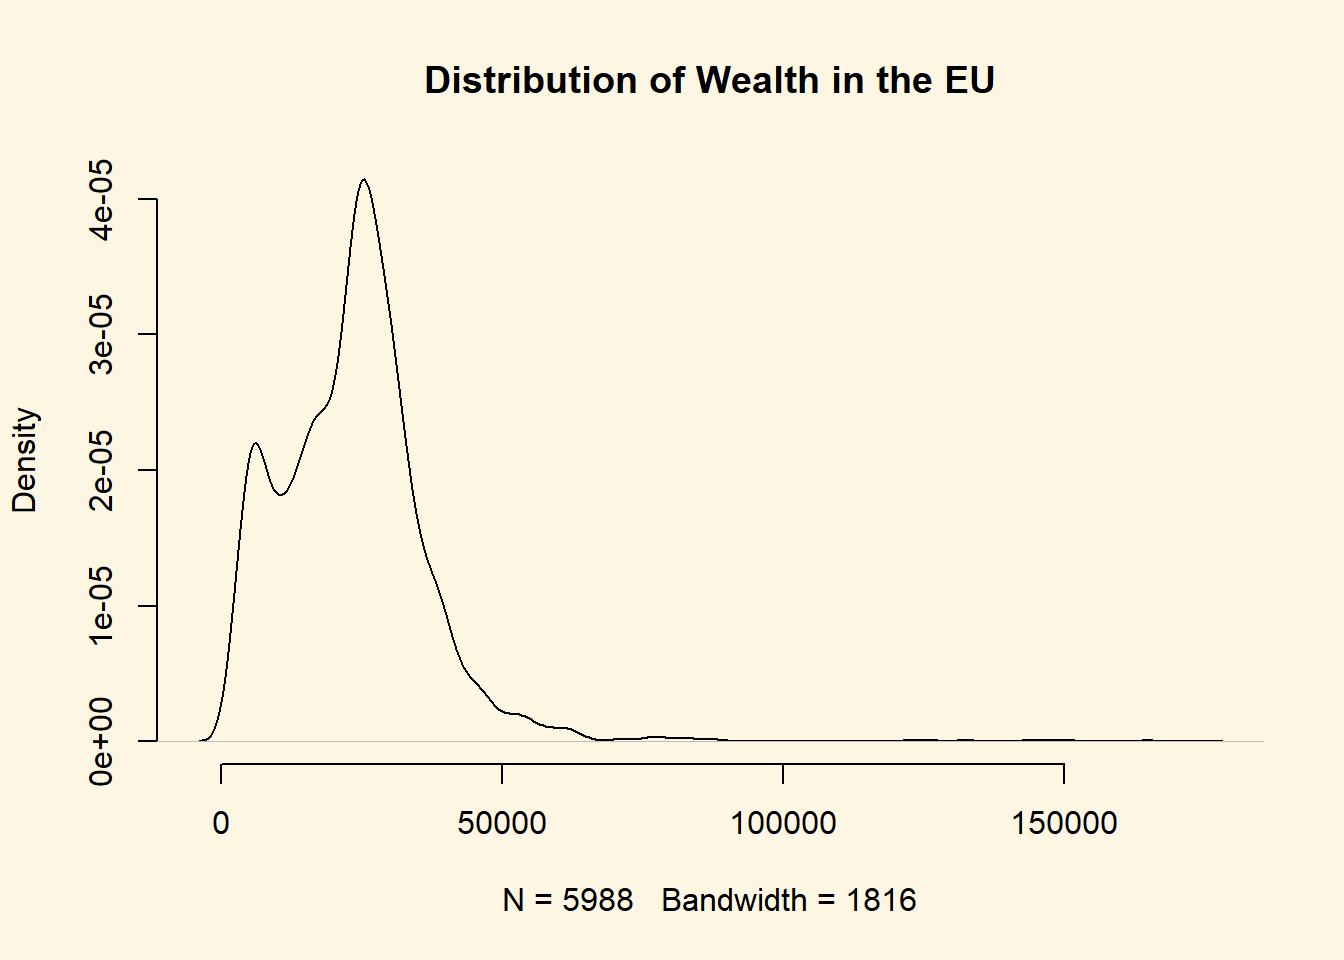
\includegraphics{r102_files/figure-latex/unnamed-chunk-36-1.pdf}

Is this distribution right-skewed or positively skewed? Put differently, are there a few observations that are very wealthy but most are not? To illustrate let's add both the median and the mean to the plot. Recall that the mean is susceptible to outliers and hence in a right-skewed distribution the mean is greater than the median.

\begin{Shaded}
\begin{Highlighting}[]
\KeywordTok{lines}\NormalTok{(}\DataTypeTok{x =} \KeywordTok{rep}\NormalTok{(}\KeywordTok{mean}\NormalTok{(eu}\OperatorTok{$}\NormalTok{wealth),}\DecValTok{10}\NormalTok{), }\DataTypeTok{y =} \KeywordTok{seq}\NormalTok{(}\DecValTok{0}\NormalTok{, }\FloatTok{4e-05}\NormalTok{, }\DataTypeTok{length.out =} \DecValTok{10}\NormalTok{), }\DataTypeTok{col =} \StringTok{"red"}\NormalTok{, }\DataTypeTok{lwd =} \DecValTok{2}\NormalTok{)}
\KeywordTok{lines}\NormalTok{(}\DataTypeTok{x =} \KeywordTok{rep}\NormalTok{(}\KeywordTok{median}\NormalTok{(eu}\OperatorTok{$}\NormalTok{wealth),}\DecValTok{10}\NormalTok{), }\DataTypeTok{y =} \KeywordTok{seq}\NormalTok{(}\DecValTok{0}\NormalTok{, }\FloatTok{4e-05}\NormalTok{, }\DataTypeTok{length.out =} \DecValTok{10}\NormalTok{), }\DataTypeTok{col =} \StringTok{"green"}\NormalTok{, }\DataTypeTok{lwd =} \DecValTok{2}\NormalTok{)}
\KeywordTok{legend}\NormalTok{(}\StringTok{"topright"}\NormalTok{, }\KeywordTok{c}\NormalTok{(}\StringTok{"Mean"}\NormalTok{, }\StringTok{"Median"}\NormalTok{),  }\DataTypeTok{col =} \KeywordTok{c}\NormalTok{(}\StringTok{"red"}\NormalTok{, }\StringTok{"green"}\NormalTok{), }\DataTypeTok{lwd =} \DecValTok{2}\NormalTok{)}
\end{Highlighting}
\end{Shaded}

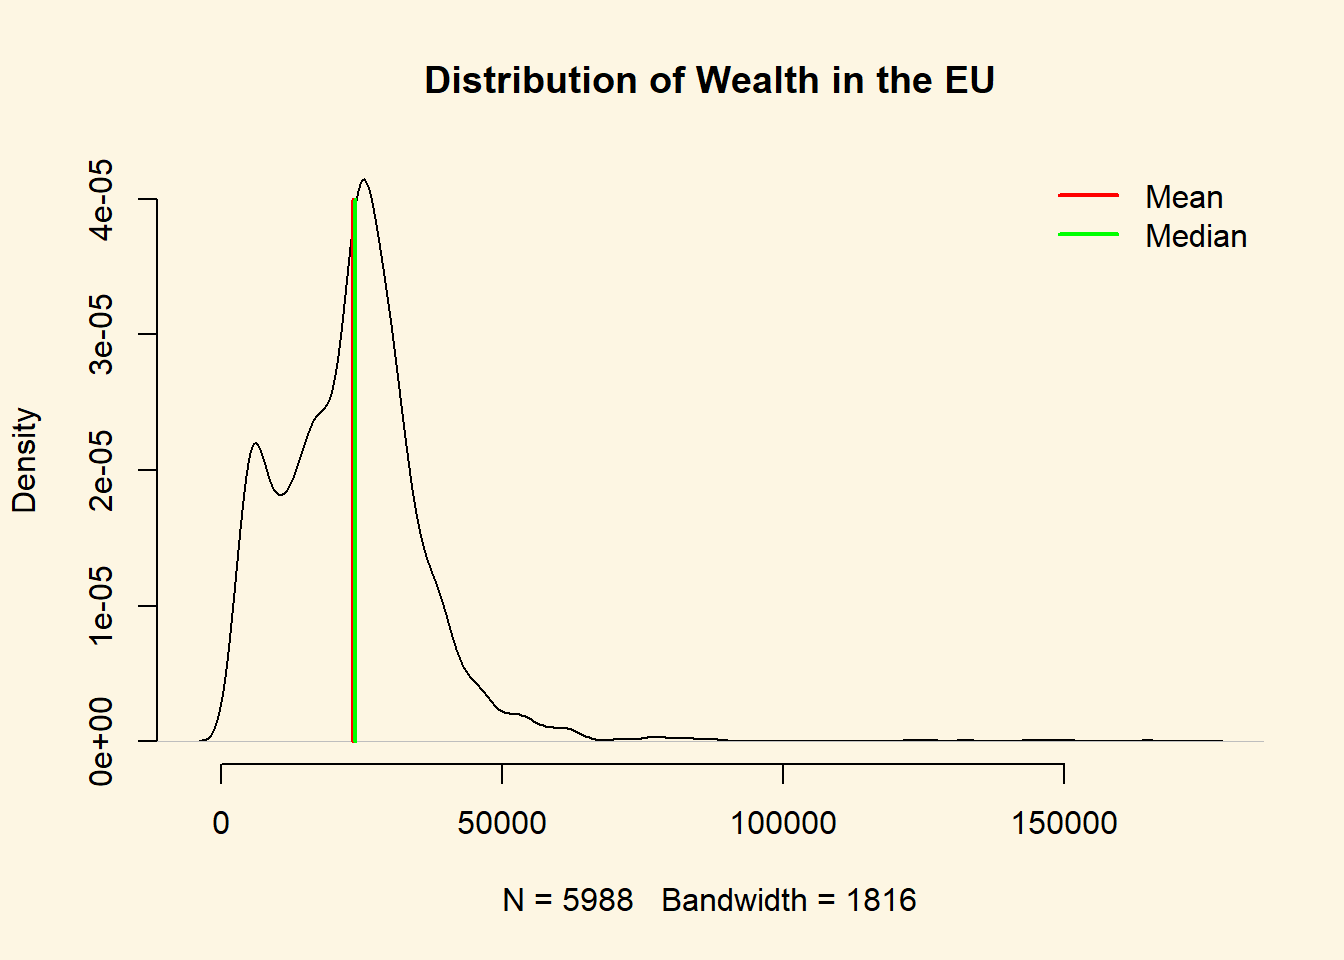
\includegraphics{r102_files/figure-latex/unnamed-chunk-38-1.pdf}

In this case median and mean are relatively close together, pointing to a relatively symmetric distribution. Keep in mind though that our unit of observation is the region-year. For instance, Essex in 1994.

Let's plot over-time development of \texttt{wealth} in Essex. On the x-axis, we plot time and on the y-axis, we plot \texttt{wealth}.

\begin{Shaded}
\begin{Highlighting}[]
\KeywordTok{plot}\NormalTok{(}
  \DataTypeTok{x =}\NormalTok{ eu}\OperatorTok{$}\NormalTok{year[eu}\OperatorTok{$}\NormalTok{region_name}\OperatorTok{==}\StringTok{"Essex"}\NormalTok{],}
  \DataTypeTok{y =}\NormalTok{ eu}\OperatorTok{$}\NormalTok{wealth[eu}\OperatorTok{$}\NormalTok{region_name}\OperatorTok{==}\StringTok{"Essex"}\NormalTok{],}
  \DataTypeTok{xlab =} \StringTok{""}\NormalTok{,}
  \DataTypeTok{ylab =} \StringTok{"Wealth in Euro"}\NormalTok{,}
  \DataTypeTok{main =} \StringTok{"GDP per person in Essex adjusted by prices"}\NormalTok{,}
  \DataTypeTok{bty =} \StringTok{"n"}\NormalTok{,}
  \DataTypeTok{col =} \StringTok{"darkgrey"}\NormalTok{,}
  \DataTypeTok{pch =} \DecValTok{16}\NormalTok{,}
  \DataTypeTok{cex =} \FloatTok{1.5}
\NormalTok{)}
\KeywordTok{lines}\NormalTok{(}\DataTypeTok{x =}\NormalTok{ eu}\OperatorTok{$}\NormalTok{year[eu}\OperatorTok{$}\NormalTok{region_name}\OperatorTok{==}\StringTok{"Essex"}\NormalTok{],}
      \DataTypeTok{y =}\NormalTok{ eu}\OperatorTok{$}\NormalTok{wealth[eu}\OperatorTok{$}\NormalTok{region_name}\OperatorTok{==}\StringTok{"Essex"}\NormalTok{],}
      \DataTypeTok{lwd =} \DecValTok{2}\NormalTok{,}
      \DataTypeTok{col =} \StringTok{"darkgrey"}\NormalTok{)}
\end{Highlighting}
\end{Shaded}

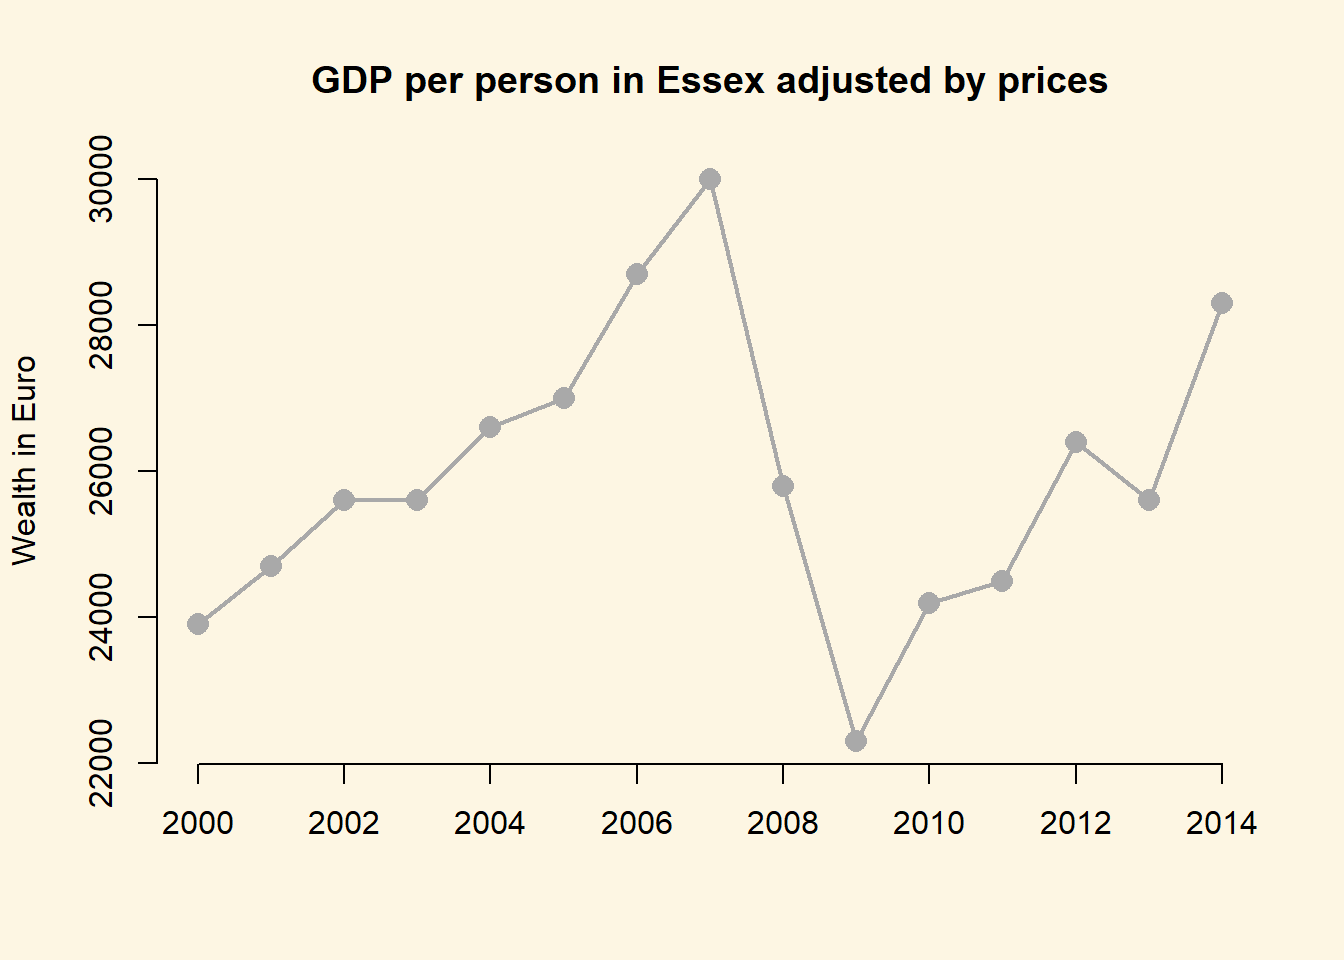
\includegraphics{r102_files/figure-latex/unnamed-chunk-39-1.pdf}

It seems that per person wealth in Essex was not quite back at pre financial crisis levels in 2014. We might want to compare Essex to the rest of the UK. Doing so efficiently means that we have to aggregate wealth data to the UK level for each year. We could write code for this but doing such manipulations is one strong suits of the tidyverse which we introduce in the next part of this course.

\hypertarget{tidyverse-introduction}{%
\section{Tidyverse introduction}\label{tidyverse-introduction}}

\hypertarget{seminar}{%
\subsection{Seminar}\label{seminar}}

\hypertarget{introduction-to-the-tidyverse}{%
\subsubsection{Introduction to the tidyverse}\label{introduction-to-the-tidyverse}}

The \texttt{tidyverse} package makes it easier to pre-process data. The package attempts to make it easier to apply operations that would otherwise require a substantial amount of coding. The syntax of the \texttt{tidyverse} is meant to be more intuitive than base R syntax but that also means that you have to learn new syntax. Working with the tidyverse is a matter of taste. A great resource for learning \texttt{tidyverse} and R is the book \href{https://r4ds.had.co.nz/}{R for data science} which is freely available.

Before getting started, we first need to install the \texttt{tidyverse} package like so: \texttt{install.packages("tidyverse")}. You only need to install once. However, doing this again is not a mistake. In fact, R, RStudio and R packages are regularly updated. It is good practice to update all of these on your computer as well. Just remember never to update before a deadline!

\begin{Shaded}
\begin{Highlighting}[]
\CommentTok{# clear workspace}
\KeywordTok{rm}\NormalTok{(}\DataTypeTok{list =} \KeywordTok{ls}\NormalTok{())}

\CommentTok{# load tidyverse package}
\KeywordTok{library}\NormalTok{(tidyverse)}
\end{Highlighting}
\end{Shaded}

Let's check whether we have updates available by runinng \texttt{tidyverse\_update()}

\begin{Shaded}
\begin{Highlighting}[]
\CommentTok{# check for available updates}
\KeywordTok{tidyverse_update}\NormalTok{()}
\end{Highlighting}
\end{Shaded}

\begin{verbatim}
The following packages are out of date:
  
* httr   (1.4.0 -> 1.4.1)
* modelr (0.1.4 -> 0.1.5)
* tidyr  (0.8.3 -> 1.0.0)
* xml2   (1.2.0 -> 1.2.2)

Start a clean R session then run:
install.packages(c("httr", "modelr", "tidyr", "xml2"))
\end{verbatim}

R tells us that several packages are in indeed out of data (this may be different on your computer - it's possible that everything is up to date on your machine). Below, we update according to the console message.

\begin{Shaded}
\begin{Highlighting}[]
\KeywordTok{install.packages}\NormalTok{(}\KeywordTok{c}\NormalTok{(}\StringTok{"httr"}\NormalTok{, }\StringTok{"modelr"}\NormalTok{, }\StringTok{"tidyr"}\NormalTok{, }\StringTok{"xml2"}\NormalTok{))}
\KeywordTok{tidyverse_update}\NormalTok{()}
\end{Highlighting}
\end{Shaded}

\begin{verbatim}
All tidyverse packages up-to-date
\end{verbatim}

Now, everything is updated correctly.

Let's re-load the EU data set that we used previously.

Download Data

\begin{Shaded}
\begin{Highlighting}[]
\NormalTok{eu <-}\StringTok{ }\KeywordTok{read.csv}\NormalTok{(}\StringTok{"qog_eureg_long_sep16.csv"}\NormalTok{, }\DataTypeTok{stringsAsFactors =} \OtherTok{FALSE}\NormalTok{)}
\end{Highlighting}
\end{Shaded}

\hypertarget{data-visualization-with-ggplot2}{%
\subsubsection{Data visualization with ggplot2}\label{data-visualization-with-ggplot2}}

In the previous exercise, we stopped on data illustration. Base R graphics is very powerful and you can do almost anything with it. However, it does require to write a lot of code. ggplot2 is useful because it helps us to produce good looking graphics with relative ease.

Let's create a simple scatter plot. We use the wealth variable \texttt{econ\_2gdp\_eur\_hab} and the European Quality of Government Index (EQI) --- variable name \texttt{eqi\_eqi} --- to assess whether the two are related but only for post 2010.

\begin{Shaded}
\begin{Highlighting}[]
\KeywordTok{ggplot}\NormalTok{(}\DataTypeTok{data =}\NormalTok{ eu[eu}\OperatorTok{$}\NormalTok{year }\OperatorTok{>}\DecValTok{2010}\NormalTok{,]) }\OperatorTok{+}
\StringTok{    }\KeywordTok{geom_point}\NormalTok{(}\DataTypeTok{mapping =} \KeywordTok{aes}\NormalTok{( }\DataTypeTok{x =}\NormalTok{ eqi_eqi, }\DataTypeTok{y =}\NormalTok{ econ_2gdp_eur_hab)) }\OperatorTok{+}
\StringTok{    }\KeywordTok{labs}\NormalTok{(}\DataTypeTok{x =} \StringTok{"Quality of Government Index"}\NormalTok{, }\DataTypeTok{y =} \StringTok{"GDP per capita price adjusted"}\NormalTok{)}
\end{Highlighting}
\end{Shaded}

\begin{verbatim}
Warning: Removed 2464 rows containing missing values (geom_point).
\end{verbatim}

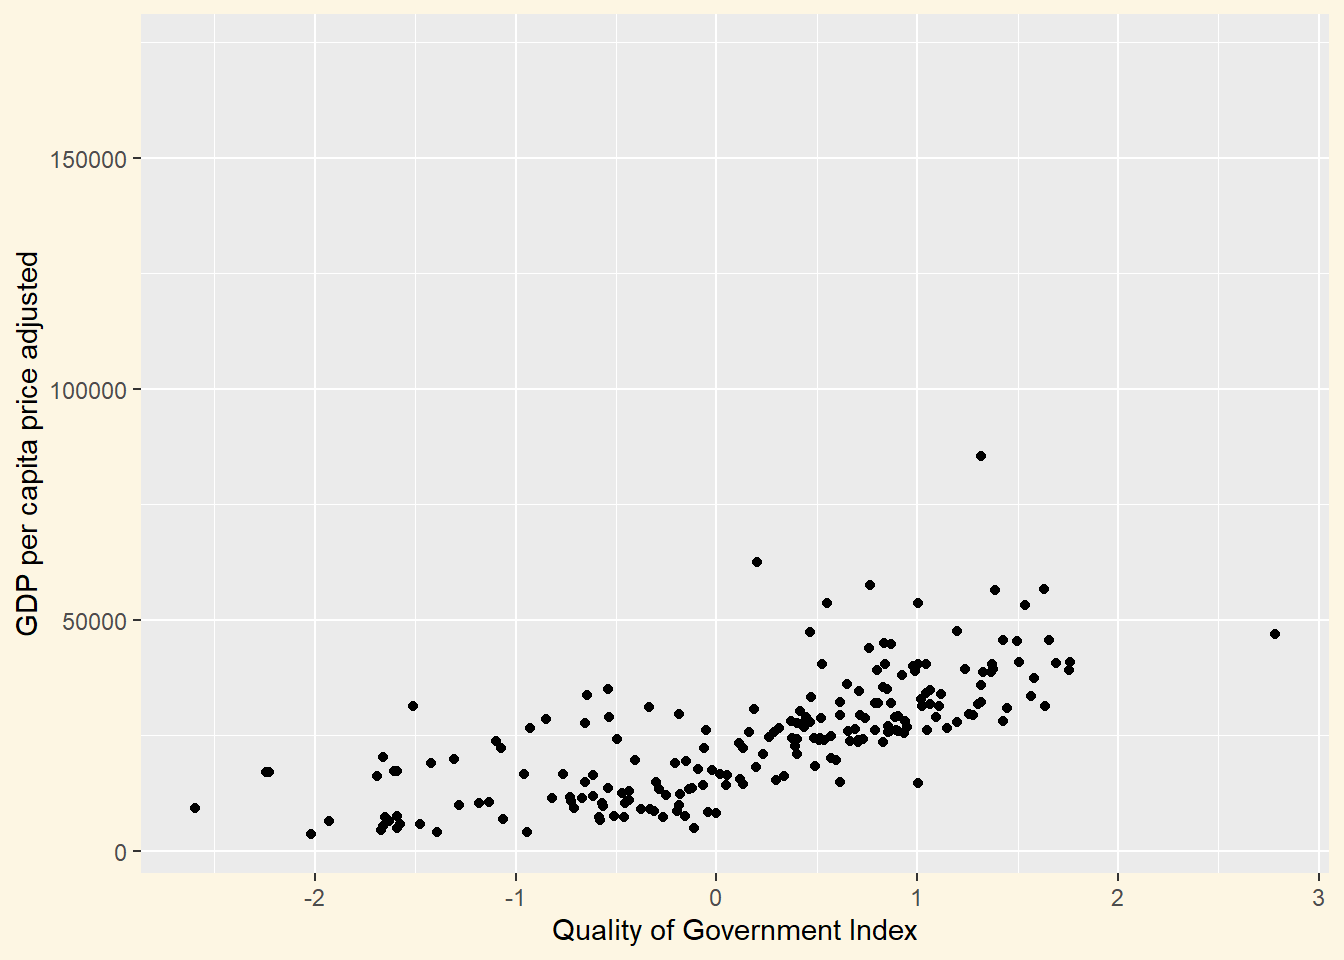
\includegraphics{r102_files/figure-latex/unnamed-chunk-47-1.pdf}

The plot looks a bit better than what we produced with base R. We also spot a slightly positive relationship. Let's walk trough the code. First, we type \texttt{ggplot()} which creates the coordinate system which we then add layers to. The argument that we supply to \texttt{ggplot()} is the data we are using. The code \texttt{ggplot(data\ =\ eu)} creates an empty plot. We then add the points or observations to the plot with the function \texttt{geom\_point()}. The argument \texttt{mapping} is necessary for ggplot to decide how variables are mapped to visuals. \texttt{mapping} is always paired with \texttt{aes()} as well as the \texttt{x} and \texttt{y} arguments which just like in base R's \texttt{plot()} function correspond to the axes. Recall that it is convention to place the independent variable on the x axis and the dependent variable on the y axis.

Let's add a third variable to the plot. Here, we use labor market statistics. The variable \texttt{unemp\_pc\_act} measures long-term unemployment as percentage of the active population. We use the variable for the color argument.

\begin{Shaded}
\begin{Highlighting}[]
\KeywordTok{ggplot}\NormalTok{(}\DataTypeTok{data =}\NormalTok{ eu[eu}\OperatorTok{$}\NormalTok{year }\OperatorTok{>}\DecValTok{2010}\NormalTok{, ]) }\OperatorTok{+}
\StringTok{    }\KeywordTok{geom_point}\NormalTok{(}\DataTypeTok{mapping =} \KeywordTok{aes}\NormalTok{( }\DataTypeTok{x =}\NormalTok{ eqi_eqi, }\DataTypeTok{y =}\NormalTok{ econ_2gdp_eur_hab, }
                              \DataTypeTok{color =}\NormalTok{ unemp_pc_act) ) }\OperatorTok{+}
\StringTok{    }\KeywordTok{labs}\NormalTok{(}\DataTypeTok{x =} \StringTok{"Quality of Government Index"}\NormalTok{, }\DataTypeTok{y =} \StringTok{"GDP per capita price adjusted"}\NormalTok{)}
\end{Highlighting}
\end{Shaded}

\begin{verbatim}
Warning: Removed 2464 rows containing missing values (geom_point).
\end{verbatim}

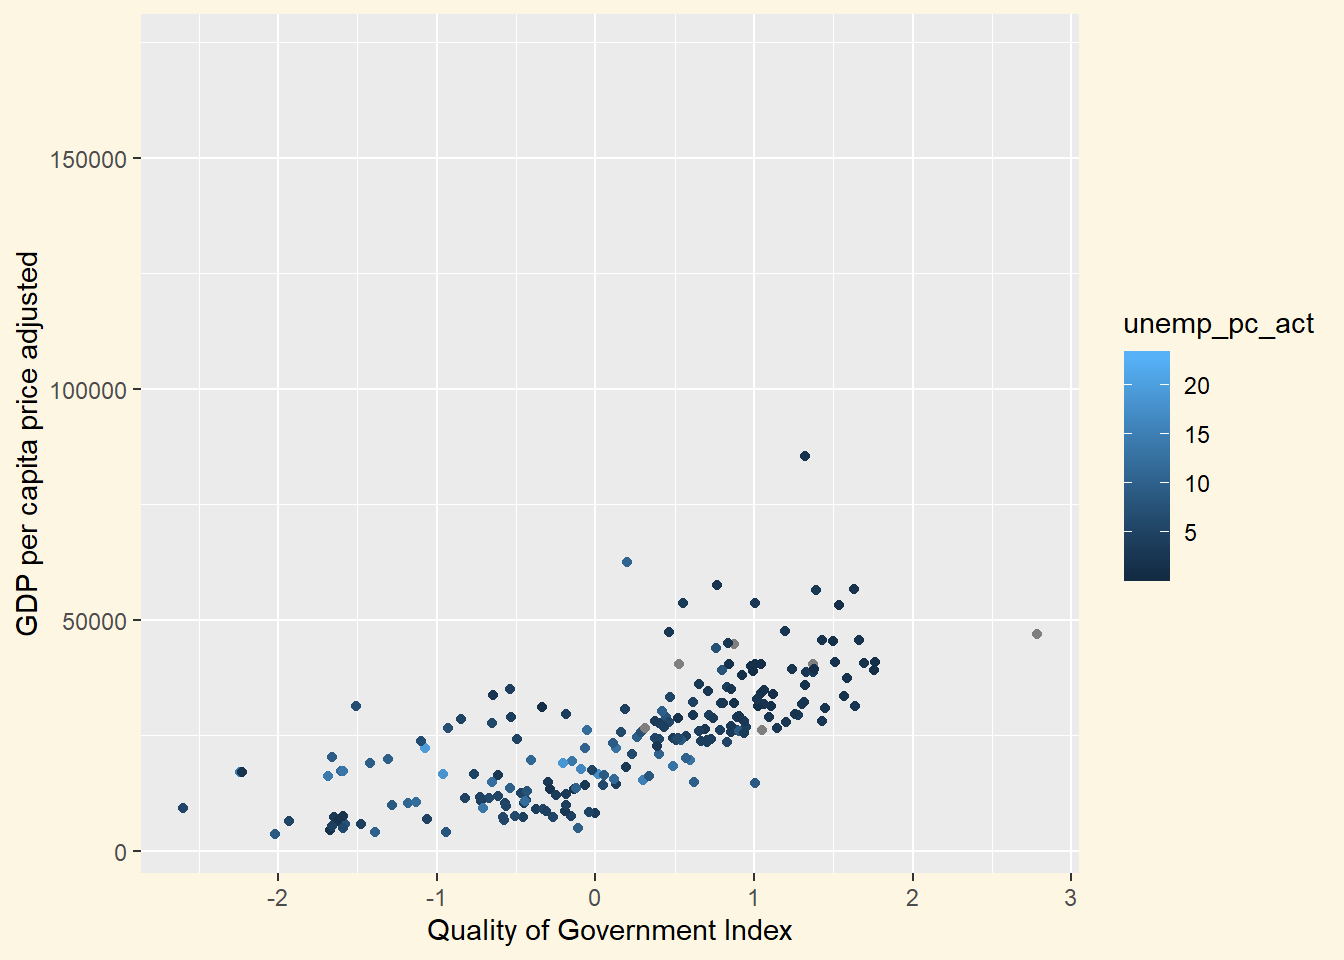
\includegraphics{r102_files/figure-latex/unnamed-chunk-49-1.pdf}

The lighter shading corresponds to more unemployment. Using unemployment does not shed a lot of light on the relationship between the variables. It does seem like places with more unemployment cluster at the lower end of the governance index and they correspond with less per capita wealth which is to be expected.

Instead of using a third variable on color, we could use it on the size of the points. For instance, population size is often applied here, making larger units more prominent. Let's use the total population variable for the size of the points.

\begin{Shaded}
\begin{Highlighting}[]
\KeywordTok{ggplot}\NormalTok{(}\DataTypeTok{data =}\NormalTok{ eu[eu}\OperatorTok{$}\NormalTok{year }\OperatorTok{>}\DecValTok{2010}\NormalTok{, ]) }\OperatorTok{+}
\StringTok{    }\KeywordTok{geom_point}\NormalTok{(}\DataTypeTok{mapping =} \KeywordTok{aes}\NormalTok{( }\DataTypeTok{x =}\NormalTok{ eqi_eqi, }\DataTypeTok{y =}\NormalTok{ econ_2gdp_eur_hab, }\DataTypeTok{color =}\NormalTok{ unemp_pc_act, }
                              \DataTypeTok{size =}\NormalTok{ demo_d2jan_t) ) }\OperatorTok{+}
\StringTok{    }\KeywordTok{labs}\NormalTok{(}\DataTypeTok{x =} \StringTok{"Quality of Government Index"}\NormalTok{, }\DataTypeTok{y =} \StringTok{"GDP per capita price adjusted"}\NormalTok{)}
\end{Highlighting}
\end{Shaded}

\begin{verbatim}
Warning: Removed 2464 rows containing missing values (geom_point).
\end{verbatim}

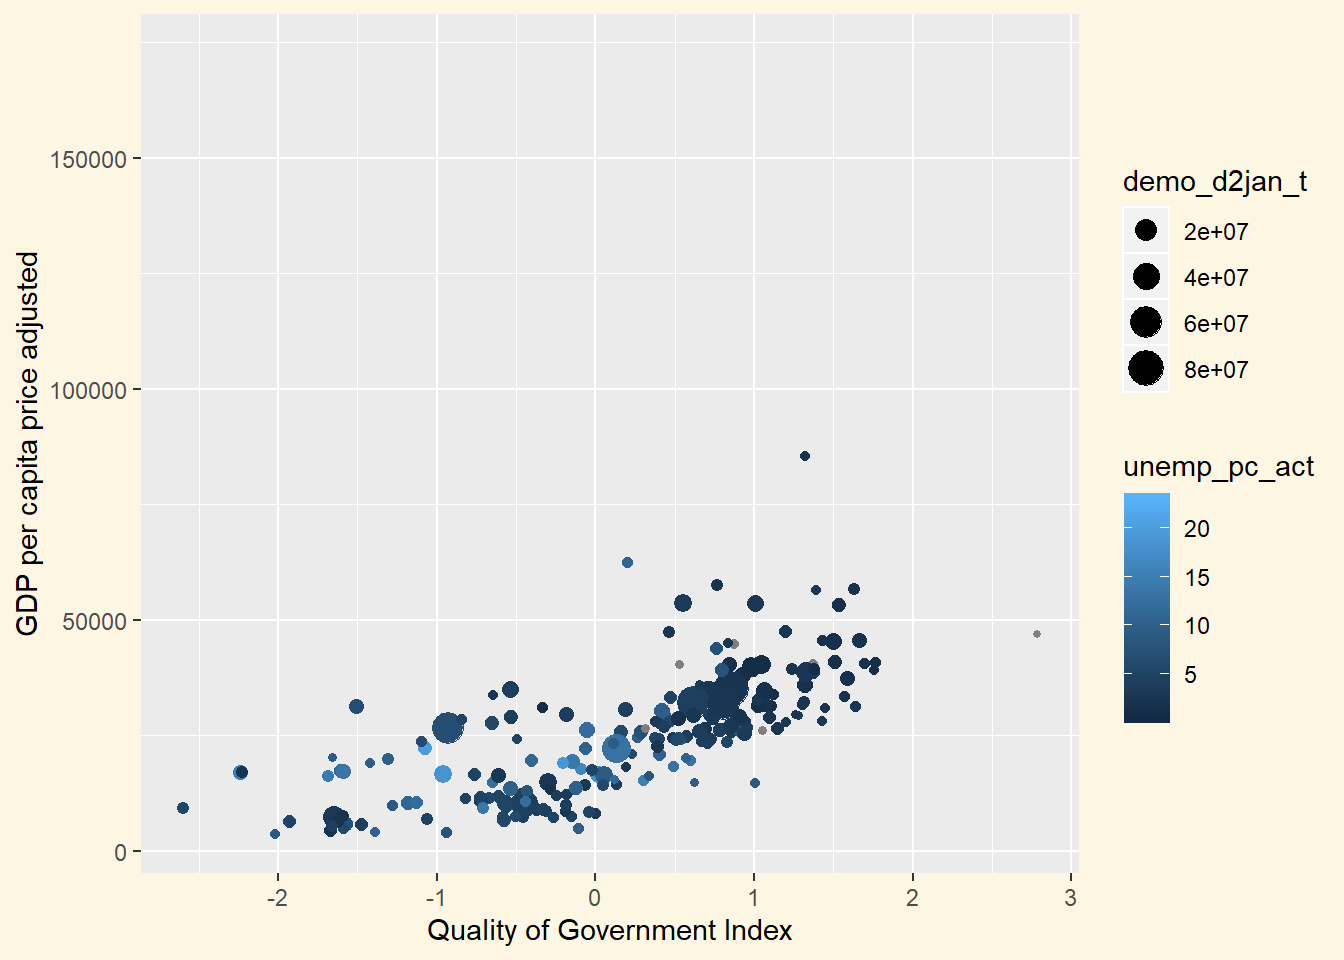
\includegraphics{r102_files/figure-latex/unnamed-chunk-51-1.pdf}

Let's evaluate whether the relationship between the governance index and wealth holds within countries. We can use \textbf{facets} to create multiple plots where the splots are split by a variable like, for instance, country.

\begin{Shaded}
\begin{Highlighting}[]
\KeywordTok{ggplot}\NormalTok{(}\DataTypeTok{data =}\NormalTok{ eu) }\OperatorTok{+}
\StringTok{    }\KeywordTok{geom_point}\NormalTok{(}\DataTypeTok{mapping =} \KeywordTok{aes}\NormalTok{( }\DataTypeTok{x =}\NormalTok{ eqi_eqi, }\DataTypeTok{y =}\NormalTok{ econ_2gdp_eur_hab)) }\OperatorTok{+}
\StringTok{    }\KeywordTok{facet_wrap}\NormalTok{(}\OperatorTok{~}\StringTok{ }\NormalTok{NUTS0, }\DataTypeTok{nrow =} \DecValTok{5}\NormalTok{)}
\end{Highlighting}
\end{Shaded}

\begin{verbatim}
Warning: Removed 13469 rows containing missing values (geom_point).
\end{verbatim}

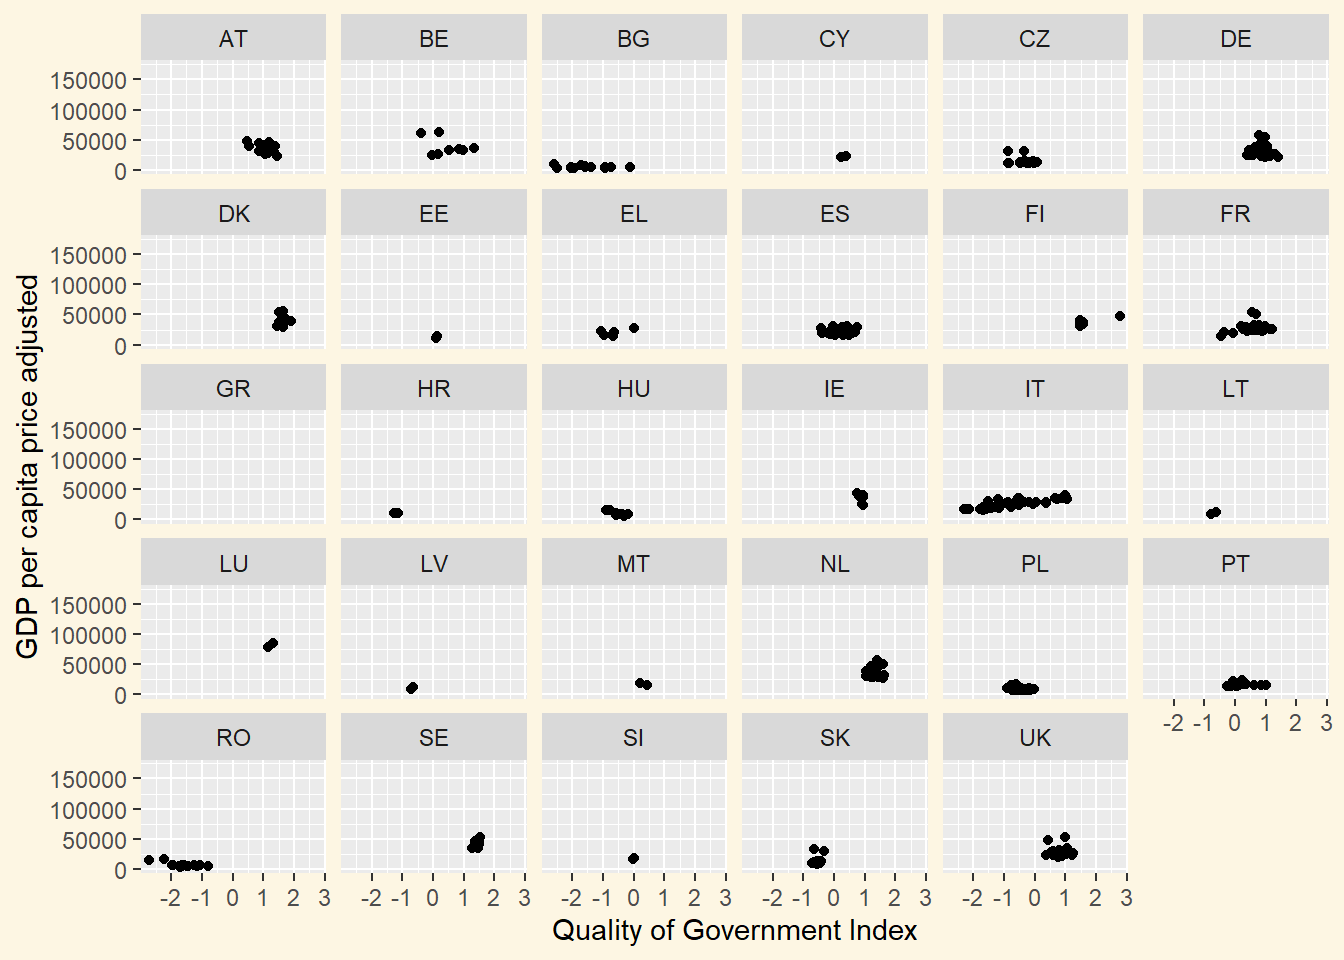
\includegraphics{r102_files/figure-latex/unnamed-chunk-53-1.pdf}

The variable to split the plot by should be discrete rather than continuous. It is diffcult to see much on facet plots, when the splitting variable has many categories as in this case. We see, however that especially in Italy there are large differences beteween the quality of governance.

In our initial plot, we were interested in the relationship between governance and the wealth. Let's add a linear regression line including the confidence interval to the plot.

\begin{Shaded}
\begin{Highlighting}[]
\KeywordTok{ggplot}\NormalTok{(eu, }\KeywordTok{aes}\NormalTok{(}\DataTypeTok{x =}\NormalTok{ eqi_eqi, }\DataTypeTok{y =}\NormalTok{ econ_2gdp_eur_hab)) }\OperatorTok{+}\StringTok{ }
\StringTok{  }\KeywordTok{geom_point}\NormalTok{() }\OperatorTok{+}
\StringTok{  }\KeywordTok{geom_smooth}\NormalTok{(}\DataTypeTok{method =}\NormalTok{ lm) }\OperatorTok{+}
\StringTok{    }\KeywordTok{labs}\NormalTok{(}\DataTypeTok{x =} \StringTok{"Quality of Government Index"}\NormalTok{, }\DataTypeTok{y =} \StringTok{"GDP per capita price adjusted"}\NormalTok{)}
\end{Highlighting}
\end{Shaded}

\begin{verbatim}
Warning: Removed 13469 rows containing non-finite values (stat_smooth).
\end{verbatim}

\begin{verbatim}
Warning: Removed 13469 rows containing missing values (geom_point).
\end{verbatim}

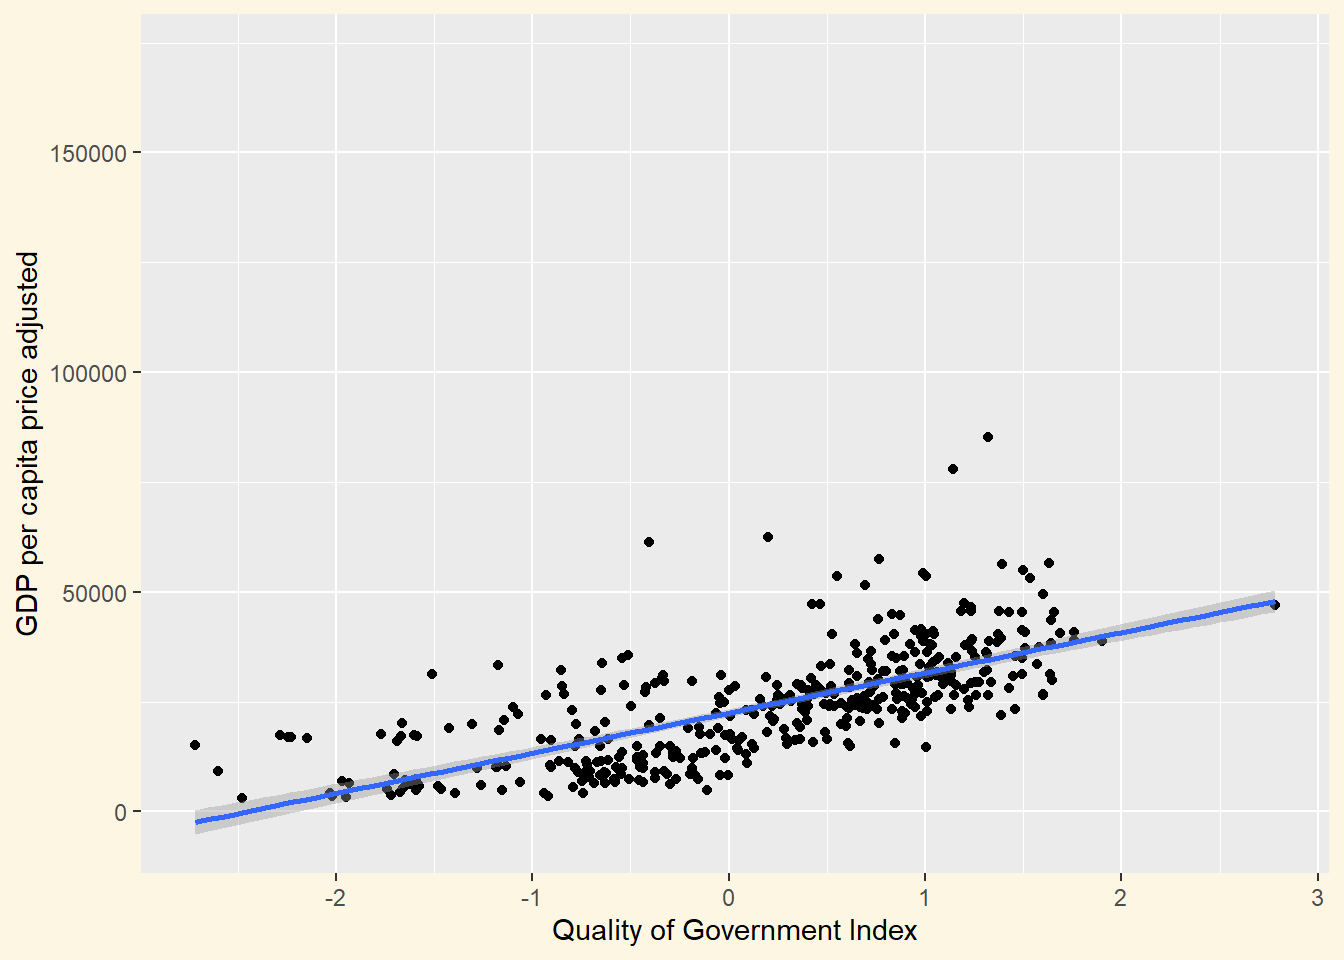
\includegraphics{r102_files/figure-latex/unnamed-chunk-55-1.pdf}

This was useful. Let's say we have a more complex model. To illustrate this, we quickly load the \texttt{world.data} data set.

Download Data

\begin{Shaded}
\begin{Highlighting}[]
\NormalTok{world.data <-}\StringTok{ }\KeywordTok{read.csv}\NormalTok{(}\StringTok{"QoG2012.csv"}\NormalTok{)}
\end{Highlighting}
\end{Shaded}

Now, we regress quality of life measured by the United Nations Human Development Index on wealth measured as GDP per capita. We fit one linear model, one quadratic model and one log transformed model. We then make predictions including confidence intervals and add them to the data set. We then plot the results using ggplot.

We need some additional data manipulation skills which we will cover as we go along. Specifically, we select a subset of the data set and we reshape the data set into long format.

\begin{Shaded}
\begin{Highlighting}[]
\CommentTok{# drop missings}
\NormalTok{world.data <-}\StringTok{ }\NormalTok{world.data[ }\OperatorTok{!}\KeywordTok{is.na}\NormalTok{(world.data}\OperatorTok{$}\NormalTok{wdi_gdpc) }\OperatorTok{&}\StringTok{ }\OperatorTok{!}\KeywordTok{is.na}\NormalTok{(world.data}\OperatorTok{$}\NormalTok{undp_hdi), ]}

\CommentTok{# run regressions}
\NormalTok{m1 <-}\StringTok{ }\KeywordTok{glm}\NormalTok{(undp_hdi }\OperatorTok{~}\StringTok{ }\NormalTok{wdi_gdpc, }\DataTypeTok{data =}\NormalTok{ world.data, }\DataTypeTok{family =} \StringTok{"gaussian"}\NormalTok{)}
\NormalTok{m2 <-}\StringTok{ }\KeywordTok{glm}\NormalTok{(undp_hdi }\OperatorTok{~}\StringTok{ }\KeywordTok{poly}\NormalTok{(wdi_gdpc,}\DecValTok{2}\NormalTok{), }\DataTypeTok{data =}\NormalTok{ world.data, }\DataTypeTok{family =} \StringTok{"gaussian"}\NormalTok{)}
\NormalTok{m3 <-}\StringTok{ }\KeywordTok{glm}\NormalTok{(undp_hdi }\OperatorTok{~}\StringTok{ }\KeywordTok{log}\NormalTok{(wdi_gdpc), }\DataTypeTok{data =}\NormalTok{ world.data, }\DataTypeTok{family =} \StringTok{"gaussian"}\NormalTok{)}

\CommentTok{# make predictions}
\NormalTok{preds1 <-}\StringTok{ }\KeywordTok{predict}\NormalTok{(m1, }\DataTypeTok{se.fit =} \OtherTok{TRUE}\NormalTok{)}
\NormalTok{preds2 <-}\StringTok{ }\KeywordTok{predict}\NormalTok{(m2, }\DataTypeTok{se.fit =} \OtherTok{TRUE}\NormalTok{)}
\NormalTok{preds3 <-}\StringTok{ }\KeywordTok{predict}\NormalTok{(m3, }\DataTypeTok{se.fit =} \OtherTok{TRUE}\NormalTok{)}

\CommentTok{## add point estimates and CIs to the world.data data set}

\CommentTok{# model 1}
\NormalTok{world.data}\OperatorTok{$}\NormalTok{bestguess1 <-}\StringTok{ }\NormalTok{preds1}\OperatorTok{$}\NormalTok{fit}
\NormalTok{world.data}\OperatorTok{$}\NormalTok{lowerbound1 <-}\StringTok{ }\NormalTok{preds1}\OperatorTok{$}\NormalTok{fit }\OperatorTok{-}\StringTok{ }\FloatTok{1.96} \OperatorTok{*}\StringTok{ }\NormalTok{preds1}\OperatorTok{$}\NormalTok{se.fit}
\NormalTok{world.data}\OperatorTok{$}\NormalTok{upperbound1 <-}\StringTok{ }\NormalTok{preds1}\OperatorTok{$}\NormalTok{fit }\OperatorTok{+}\StringTok{ }\FloatTok{1.96} \OperatorTok{*}\StringTok{ }\NormalTok{preds1}\OperatorTok{$}\NormalTok{se.fit}

\CommentTok{# model 2}
\NormalTok{world.data}\OperatorTok{$}\NormalTok{bestguess2 <-}\StringTok{ }\NormalTok{preds2}\OperatorTok{$}\NormalTok{fit}
\NormalTok{world.data}\OperatorTok{$}\NormalTok{lowerbound2 <-}\StringTok{ }\NormalTok{preds2}\OperatorTok{$}\NormalTok{fit }\OperatorTok{-}\StringTok{ }\FloatTok{1.96} \OperatorTok{*}\StringTok{ }\NormalTok{preds2}\OperatorTok{$}\NormalTok{se.fit}
\NormalTok{world.data}\OperatorTok{$}\NormalTok{upperbound2 <-}\StringTok{ }\NormalTok{preds2}\OperatorTok{$}\NormalTok{fit }\OperatorTok{+}\StringTok{ }\FloatTok{1.96} \OperatorTok{*}\StringTok{ }\NormalTok{preds2}\OperatorTok{$}\NormalTok{se.fit}

\CommentTok{# model 3}
\NormalTok{world.data}\OperatorTok{$}\NormalTok{bestguess3 <-}\StringTok{ }\NormalTok{preds3}\OperatorTok{$}\NormalTok{fit}
\NormalTok{world.data}\OperatorTok{$}\NormalTok{lowerbound3 <-}\StringTok{ }\NormalTok{preds3}\OperatorTok{$}\NormalTok{fit }\OperatorTok{-}\StringTok{ }\FloatTok{1.96} \OperatorTok{*}\StringTok{ }\NormalTok{preds3}\OperatorTok{$}\NormalTok{se.fit}
\NormalTok{world.data}\OperatorTok{$}\NormalTok{upperbound3 <-}\StringTok{ }\NormalTok{preds3}\OperatorTok{$}\NormalTok{fit }\OperatorTok{+}\StringTok{ }\FloatTok{1.96} \OperatorTok{*}\StringTok{ }\NormalTok{preds3}\OperatorTok{$}\NormalTok{se.fit}

\CommentTok{# selecting a subset of variables}
\NormalTok{plot.data <-}\StringTok{ }\NormalTok{dplyr}\OperatorTok{::}\KeywordTok{select}\NormalTok{(}
\NormalTok{  world.data,}
  \StringTok{"undp_hdi"}\NormalTok{,}
  \StringTok{"wdi_gdpc"}\NormalTok{,}
  \StringTok{"bestguess1"}\NormalTok{,}\StringTok{"lowerbound1"}\NormalTok{,}\StringTok{"upperbound1"}\NormalTok{,}
  \StringTok{"bestguess2"}\NormalTok{,}\StringTok{"lowerbound2"}\NormalTok{,}\StringTok{"upperbound2"}\NormalTok{,}
  \StringTok{"bestguess3"}\NormalTok{,}\StringTok{"lowerbound3"}\NormalTok{,}\StringTok{"upperbound3"}\NormalTok{)}

\CommentTok{# reshaping the data set}
\NormalTok{plot.data <-}\StringTok{ }\KeywordTok{reshape}\NormalTok{(plot.data, }\DataTypeTok{direction =} \StringTok{"long"}\NormalTok{,}
        \DataTypeTok{varying =} \KeywordTok{c}\NormalTok{(}\StringTok{"bestguess1"}\NormalTok{,}\StringTok{"lowerbound1"}\NormalTok{,}\StringTok{"upperbound1"}\NormalTok{,}
                    \StringTok{"bestguess2"}\NormalTok{,}\StringTok{"lowerbound2"}\NormalTok{,}\StringTok{"upperbound2"}\NormalTok{,}
                    \StringTok{"bestguess3"}\NormalTok{,}\StringTok{"lowerbound3"}\NormalTok{,}\StringTok{"upperbound3"}\NormalTok{),}
        \DataTypeTok{timevar =} \StringTok{"Model"}\NormalTok{,}
        \DataTypeTok{times =} \KeywordTok{c}\NormalTok{(}\StringTok{"1"}\NormalTok{,}\StringTok{"2"}\NormalTok{,}\StringTok{"3"}\NormalTok{),}
        \DataTypeTok{v.names =} \KeywordTok{c}\NormalTok{(}\StringTok{"bestguess"}\NormalTok{,}\StringTok{"lowerbound"}\NormalTok{,}\StringTok{"upperbound"}\NormalTok{),}
        \DataTypeTok{idvar =} \KeywordTok{c}\NormalTok{(}\StringTok{"undp_hdi"}\NormalTok{,}\StringTok{"wdi_gdpc"}\NormalTok{))}

\CommentTok{# renaming the rownames of the data set}
\KeywordTok{row.names}\NormalTok{(plot.data) <-}\StringTok{ }\KeywordTok{seq}\NormalTok{(}\DecValTok{1}\OperatorTok{:}\KeywordTok{nrow}\NormalTok{(plot.data))}

\CommentTok{# changing the grouping id into a factor}
\NormalTok{plot.data}\OperatorTok{$}\NormalTok{Model <-}\StringTok{ }\KeywordTok{factor}\NormalTok{(plot.data}\OperatorTok{$}\NormalTok{Model, }\DataTypeTok{levels =} \KeywordTok{c}\NormalTok{(}\DecValTok{1}\NormalTok{,}\DecValTok{2}\NormalTok{,}\DecValTok{3}\NormalTok{), }\DataTypeTok{labels =} \KeywordTok{c}\NormalTok{(}\StringTok{"Linear"}\NormalTok{, }\StringTok{"Quadratic"}\NormalTok{, }\StringTok{"Log"}\NormalTok{))}

\KeywordTok{ggplot}\NormalTok{(plot.data, }\KeywordTok{aes}\NormalTok{(}\DataTypeTok{x =}\NormalTok{ wdi_gdpc, }\DataTypeTok{y =}\NormalTok{ undp_hdi)) }\OperatorTok{+}
\StringTok{    }\KeywordTok{geom_point}\NormalTok{(}\DataTypeTok{alpha =} \FloatTok{0.6}\NormalTok{, }\DataTypeTok{color =} \StringTok{"black"}\NormalTok{) }\OperatorTok{+}
\StringTok{    }\KeywordTok{geom_line}\NormalTok{( }\KeywordTok{aes}\NormalTok{( }\DataTypeTok{y =}\NormalTok{ bestguess, }\DataTypeTok{color =}\NormalTok{ Model), }\DataTypeTok{size =} \DecValTok{1}\NormalTok{, }\DataTypeTok{alpha =} \FloatTok{0.8}\NormalTok{) }\OperatorTok{+}
\StringTok{    }\KeywordTok{geom_ribbon}\NormalTok{( }\KeywordTok{aes}\NormalTok{( }\DataTypeTok{ymin =}\NormalTok{ lowerbound, }\DataTypeTok{ymax =}\NormalTok{ upperbound, }\DataTypeTok{fill =}\NormalTok{ Model), }\DataTypeTok{alpha =} \FloatTok{0.25}\NormalTok{ ) }\OperatorTok{+}
\StringTok{    }\KeywordTok{labs}\NormalTok{( }\DataTypeTok{x =} \StringTok{"GDP per capita"}\NormalTok{, }\DataTypeTok{y =} \StringTok{"Human Development Index"}\NormalTok{, }
          \DataTypeTok{title =} \StringTok{"Relationship between wealth and quality of life"}\NormalTok{)}
\end{Highlighting}
\end{Shaded}

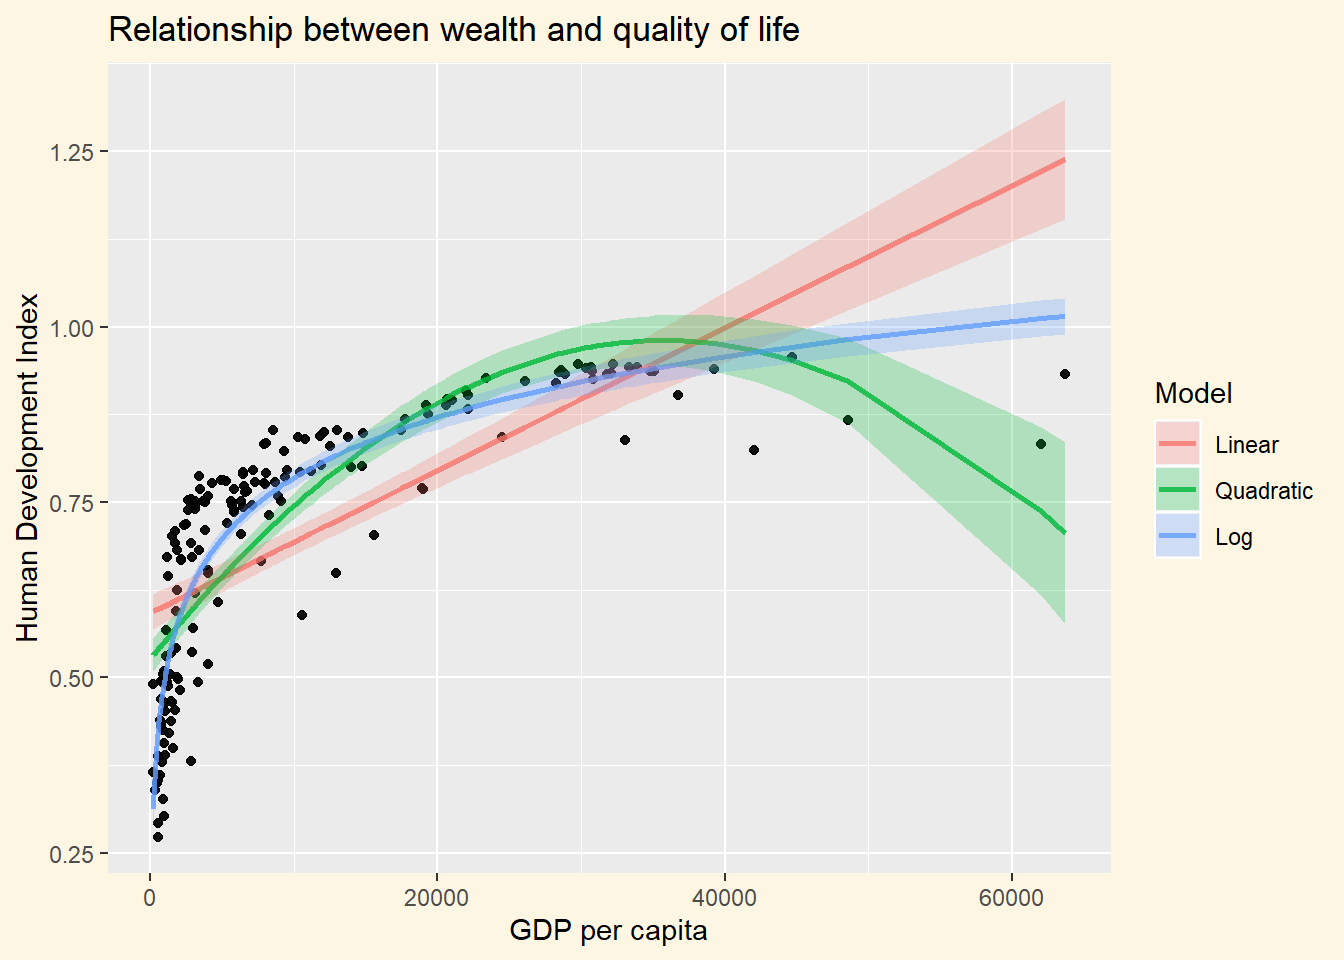
\includegraphics{r102_files/figure-latex/unnamed-chunk-58-1.pdf}

\hypertarget{renaming-variables-and-selecting-subsets}{%
\subsubsection{Renaming variables and selecting subsets}\label{renaming-variables-and-selecting-subsets}}

You may remember that renaming variables involved sub-setting and the logical evaluations. Well, this is one of the things that is quite easy to do in tidyverse. Here, we use the \texttt{rename()} function from the \texttt{dplyr} package.

Let's go back to the \texttt{eu} data set and rename the following variables:

\begin{enumerate}
\def\labelenumi{\arabic{enumi}.}
\tightlist
\item
  \texttt{NUTS0} into \texttt{country}
\item
  \texttt{region\_name} into \texttt{region}
\item
  \texttt{econ\_2gdp\_eur\_hab} into \texttt{wealth}
\item
  \texttt{eqi\_eqi} into \texttt{quality.of.government}
\end{enumerate}

\begin{Shaded}
\begin{Highlighting}[]
\NormalTok{eu.renamed <-}\StringTok{ }\KeywordTok{rename}\NormalTok{(eu,}
                     \DataTypeTok{country =}\NormalTok{ NUTS0,}
                     \DataTypeTok{region =}\NormalTok{ region_name,}
                     \DataTypeTok{wealth =}\NormalTok{ econ_2gdp_eur_hab,}
                     \DataTypeTok{quality.of.government =}\NormalTok{ eqi_eqi)}
\end{Highlighting}
\end{Shaded}

Selecting a subset is as easy as renaming. The function \texttt{select()} lets us do this easily. The function \texttt{select()} exists in multiple packages. To avoid conflicts when loading these packages at the same time, we call \texttt{dplyr::select()} to make sure we use function from the correct package.

\begin{Shaded}
\begin{Highlighting}[]
\NormalTok{eu.renamed <-}\StringTok{ }\NormalTok{dplyr}\OperatorTok{::}\KeywordTok{select}\NormalTok{(}
\NormalTok{  eu.renamed,}
\NormalTok{  country, region, wealth, quality.of.government)}
\KeywordTok{names}\NormalTok{(eu.renamed)}
\end{Highlighting}
\end{Shaded}

\begin{verbatim}
[1] "country"               "region"                "wealth"               
[4] "quality.of.government"
\end{verbatim}

Let's remove our small data set \texttt{eu.renamed}.

\begin{Shaded}
\begin{Highlighting}[]
\KeywordTok{rm}\NormalTok{(eu.renamed)}
\end{Highlighting}
\end{Shaded}

We can rename and select in one step within the \texttt{select()} function.

\begin{Shaded}
\begin{Highlighting}[]
\NormalTok{eu <-}\StringTok{ }\NormalTok{dplyr}\OperatorTok{::}\KeywordTok{select}\NormalTok{(}
\NormalTok{  eu,}
  \DataTypeTok{country =}\NormalTok{ NUTS0,}
  \DataTypeTok{region =}\NormalTok{ region_name,}
\NormalTok{  year,}
  \DataTypeTok{wealth =}\NormalTok{ econ_2gdp_eur_hab,}
  \DataTypeTok{quality.of.government =}\NormalTok{ eqi_eqi)}
\KeywordTok{summary}\NormalTok{(eu)}
\end{Highlighting}
\end{Shaded}

\begin{verbatim}
   country             region               year          wealth      
 Length:13884       Length:13884       Min.   :1990   Min.   :  1300  
 Class :character   Class :character   1st Qu.:1996   1st Qu.: 14600  
 Mode  :character   Mode  :character   Median :2002   Median : 23800  
                                       Mean   :2002   Mean   : 23450  
                                       3rd Qu.:2009   3rd Qu.: 30000  
                                       Max.   :2015   Max.   :172600  
                                                      NA's   :7896    
 quality.of.government
 Min.   :-2.719       
 1st Qu.:-0.534       
 Median : 0.368       
 Mean   : 0.184       
 3rd Qu.: 0.963       
 Max.   : 2.781       
 NA's   :13453        
\end{verbatim}

\hypertarget{aggregating-and-pipes}{%
\subsubsection{Aggregating and pipes}\label{aggregating-and-pipes}}

Our data set is on the region-year level. We want to compare countries over time. Therefore, we now aggregate our data up to the country-year level. Note that you want data in the most dis-aggregated fashion possible because aggregating to the next higher level is easy. We want to average over the regions within each country and year.

To do this we introduce two new functions and one new concept. The new concept is called the pipe and its operator is \texttt{\%\textgreater{}\%}. In our example we say first create a copy of the data set called \texttt{eu} called \texttt{eu.country.year}. We do not stop here but we continue on indicated by the pipe operator \texttt{\%\textgreater{}\%}. We then group the data set by two variables with the \texttt{group\_by()} function. The first variable that indentifies groups is the country and the second is the year. We then contiue on with the pipe operator \texttt{\%\textgreater{}\%} and finally we summarize the data within the groups using the \texttt{summarize()} function.

\begin{Shaded}
\begin{Highlighting}[]
\NormalTok{eu.country.year <-}\StringTok{ }\NormalTok{eu }\OperatorTok
\StringTok{    }\KeywordTok{group_by}\NormalTok{(country, year) }\OperatorTok
\StringTok{    }\KeywordTok{summarize}\NormalTok{(}\DataTypeTok{wealth =} \KeywordTok{mean}\NormalTok{(wealth, }\DataTypeTok{na.rm =} \OtherTok{TRUE}\NormalTok{),}
              \DataTypeTok{quality.of.government =} \KeywordTok{mean}\NormalTok{(quality.of.government, }\DataTypeTok{na.rm =} \OtherTok{TRUE}\NormalTok{))}

\KeywordTok{head}\NormalTok{(eu.country.year, }\DataTypeTok{n =} \DecValTok{15}\NormalTok{)}
\end{Highlighting}
\end{Shaded}

\begin{verbatim}
# A tibble: 15 x 4
# Groups:   country [1]
   country  year wealth quality.of.government
   <chr>   <int>  <dbl>                 <dbl>
 1 AT       1990   NaN                    NaN
 2 AT       1991   NaN                    NaN
 3 AT       1992   NaN                    NaN
 4 AT       1993   NaN                    NaN
 5 AT       1994   NaN                    NaN
 6 AT       1995   NaN                    NaN
 7 AT       1996   NaN                    NaN
 8 AT       1997   NaN                    NaN
 9 AT       1998   NaN                    NaN
10 AT       1999   NaN                    NaN
11 AT       2000 25738.                   NaN
12 AT       2001 26477.                   NaN
13 AT       2002 27138.                   NaN
14 AT       2003 27623.                   NaN
15 AT       2004 28746.                   NaN
\end{verbatim}

It turns out that we have a lot of missing data in our dataset. Our goal is to plot wealth over time. We have all the necessary parts to do this but we would like to also add an EU average. In other words, for each year we need to create a new observation that receives the value \texttt{EU} for the country variable and the average of wealth within that year and the average of quality of government within that year. We follow the same procedure as previosly.

\begin{Shaded}
\begin{Highlighting}[]
\NormalTok{eu.year <-}\StringTok{ }\NormalTok{eu.country.year }\OperatorTok
\StringTok{    }\KeywordTok{group_by}\NormalTok{(year) }\OperatorTok
\StringTok{    }\KeywordTok{summarize}\NormalTok{(}\DataTypeTok{wealth =} \KeywordTok{mean}\NormalTok{(wealth, }\DataTypeTok{na.rm =} \OtherTok{TRUE}\NormalTok{),}
              \DataTypeTok{quality.of.government =} \KeywordTok{mean}\NormalTok{(quality.of.government, }\DataTypeTok{na.rm =} \OtherTok{TRUE}\NormalTok{))}
\end{Highlighting}
\end{Shaded}

We now have two datasets which need to combine.

\hypertarget{merging-data-sets}{%
\subsubsection{Merging data sets}\label{merging-data-sets}}

We cannot just paste the data sets together because they differ in the number of columns. As a first step, we need to create a new variable in the data set \texttt{eu.year} called \texttt{country} which identifies the country in that data set.

\begin{Shaded}
\begin{Highlighting}[]
\NormalTok{eu.year}\OperatorTok{$}\NormalTok{country <-}\StringTok{ "EU"}
\NormalTok{eu.year}
\end{Highlighting}
\end{Shaded}

\begin{verbatim}
# A tibble: 26 x 4
    year wealth quality.of.government country
   <int>  <dbl>                 <dbl> <chr>  
 1  1990    NaN                   NaN EU     
 2  1991    NaN                   NaN EU     
 3  1992    NaN                   NaN EU     
 4  1993    NaN                   NaN EU     
 5  1994    NaN                   NaN EU     
 6  1995    NaN                   NaN EU     
 7  1996    NaN                   NaN EU     
 8  1997    NaN                   NaN EU     
 9  1998    NaN                   NaN EU     
10  1999    NaN                   NaN EU     
# ... with 16 more rows
\end{verbatim}

We now merge the two variables together. Recall that observations are uniquely identified by the variables \texttt{country} and \texttt{year}. We neeed to order the observations in both data sets before merging. To do this we use the \texttt{arrange()} function from the \texttt{dplyr} package. The datasets are already ordered by the country first and the year second. Let's reorder by year first and then country to illustrate how the function works.

\begin{Shaded}
\begin{Highlighting}[]
\NormalTok{eu.country.year <-}\StringTok{ }\KeywordTok{arrange}\NormalTok{(eu.country.year, year, country)}
\NormalTok{eu.year <-}\StringTok{ }\KeywordTok{arrange}\NormalTok{(eu.year, year, country)}
\KeywordTok{head}\NormalTok{(eu.country.year, }\DataTypeTok{n =} \DecValTok{20}\NormalTok{)}
\end{Highlighting}
\end{Shaded}

\begin{verbatim}
# A tibble: 20 x 4
# Groups:   country [20]
   country  year wealth quality.of.government
   <chr>   <int>  <dbl>                 <dbl>
 1 AT       1990    NaN                   NaN
 2 BE       1990    NaN                   NaN
 3 BG       1990    NaN                   NaN
 4 CY       1990    NaN                   NaN
 5 CZ       1990    NaN                   NaN
 6 DE       1990    NaN                   NaN
 7 DK       1990    NaN                   NaN
 8 EE       1990    NaN                   NaN
 9 EL       1990    NaN                   NaN
10 ES       1990    NaN                   NaN
11 FI       1990    NaN                   NaN
12 FR       1990    NaN                   NaN
13 GR       1990    NaN                   NaN
14 HR       1990    NaN                   NaN
15 HU       1990    NaN                   NaN
16 IE       1990    NaN                   NaN
17 IT       1990    NaN                   NaN
18 LT       1990    NaN                   NaN
19 LU       1990    NaN                   NaN
20 LV       1990    NaN                   NaN
\end{verbatim}

We are ready to merge. To do so, we use the \texttt{merge()} function. We have the same variables in both data sets and both are unique observations. In this case, an alternative to using \texttt{merge()} is to simply bind the data sets together row-wise like so: \texttt{rbind(eu.country.year,\ eu.year)}. However, the nice side-effect of using \texttt{merge()} is that our order by years and then countries remains intact. So the first two arguemnts of \texttt{merge()} are the names of the data sets to merge. We then specify the variables to merge by in the \texttt{by} argument and finally we need to say keep all observations that are unique to either data set with \texttt{all\ =\ TRUE}.

\begin{Shaded}
\begin{Highlighting}[]
\NormalTok{eu.join <-}\StringTok{ }\KeywordTok{merge}\NormalTok{(eu.country.year, eu.year, }\DataTypeTok{by =} \KeywordTok{intersect}\NormalTok{(}\KeywordTok{names}\NormalTok{(eu.country.year), }\KeywordTok{names}\NormalTok{(eu.year)), }\DataTypeTok{all =} \OtherTok{TRUE}\NormalTok{)}
\end{Highlighting}
\end{Shaded}

Now, you should be able to plot wealth over time on your own. The plot should show the all ``countries'' in the data set. We do not have data before 2000, so there is no point in plotting it.

\begin{Shaded}
\begin{Highlighting}[]
\KeywordTok{ggplot}\NormalTok{(eu.join[eu.join}\OperatorTok{$}\NormalTok{year}\OperatorTok{>}\DecValTok{1999}\NormalTok{,]) }\OperatorTok{+}
\StringTok{    }\KeywordTok{geom_line}\NormalTok{(}\DataTypeTok{mapping =} \KeywordTok{aes}\NormalTok{( }\DataTypeTok{x =}\NormalTok{ year, }\DataTypeTok{y =}\NormalTok{ wealth, }\DataTypeTok{col =}\NormalTok{ country))}
\end{Highlighting}
\end{Shaded}

\begin{verbatim}
Warning: Removed 45 rows containing missing values (geom_path).
\end{verbatim}

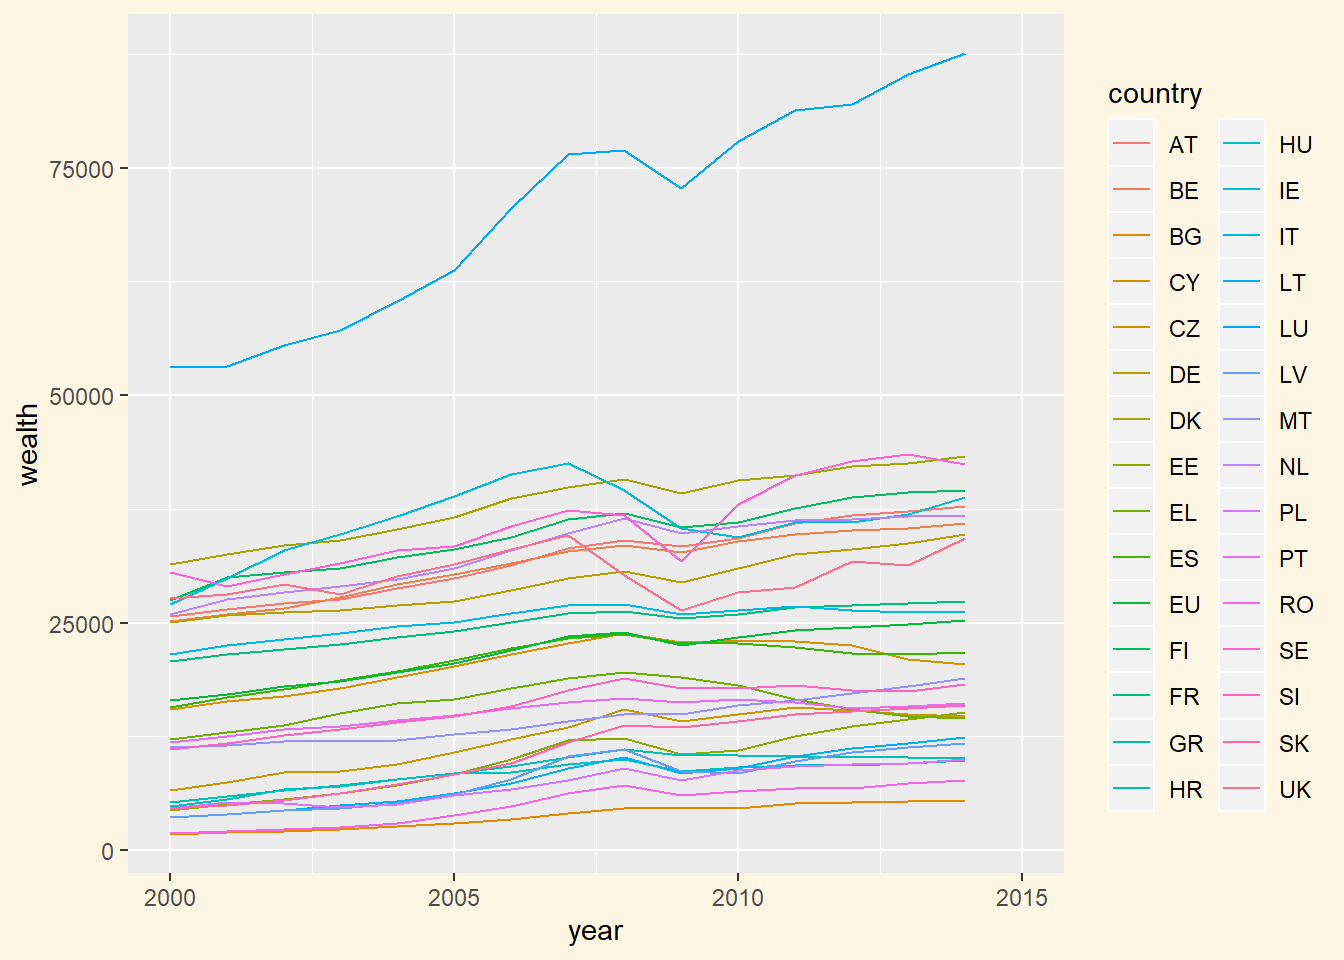
\includegraphics{r102_files/figure-latex/unnamed-chunk-69-1.pdf}

There are too many countries in this plot. Let's compare the UK with France, Italy, Belgium, Greece, Germany, and Spain. To do this, we use the \texttt{filter()} function. We also take the opportunity to filter out the missing years.

\begin{Shaded}
\begin{Highlighting}[]
\NormalTok{eu.join.small <-}\StringTok{ }\KeywordTok{filter}\NormalTok{(eu.join, country }\OperatorTok\StringTok{ }\KeywordTok{c}\NormalTok{(}\StringTok{"UK"}\NormalTok{,}\StringTok{"FR"}\NormalTok{,}\StringTok{"IT"}\NormalTok{,}\StringTok{"BE"}\NormalTok{,}\StringTok{"EL"}\NormalTok{,}\StringTok{"DE"}\NormalTok{,}\StringTok{"ES"}\NormalTok{) }\OperatorTok{&}\StringTok{ }\NormalTok{year }\OperatorTok{>}\StringTok{ }\DecValTok{1999} \OperatorTok{&}\StringTok{ }\NormalTok{year }\OperatorTok{<}\StringTok{ }\DecValTok{2015}\NormalTok{ )}
\KeywordTok{head}\NormalTok{(eu.join.small, }\DataTypeTok{n =} \DecValTok{20}\NormalTok{)}
\end{Highlighting}
\end{Shaded}

\begin{verbatim}
   country year   wealth quality.of.government
1       BE 2000 25200.00                   NaN
2       BE 2001 25900.00                   NaN
3       BE 2002 26600.00                   NaN
4       BE 2003 27793.33                   NaN
5       BE 2004 29253.33                   NaN
6       BE 2005 30300.00                   NaN
7       BE 2006 31506.67                   NaN
8       BE 2007 32873.33                   NaN
9       BE 2008 33493.33                   NaN
10      BE 2009 32720.00                   NaN
11      BE 2010 34020.00             0.2645683
12      BE 2011 34786.67                   NaN
13      BE 2012 35146.67                   NaN
14      BE 2013 35426.67             0.6278485
15      BE 2014 35993.33                   NaN
16      DE 2000 25083.64                   NaN
17      DE 2001 25789.09                   NaN
18      DE 2002 26163.64                   NaN
19      DE 2003 26347.27                   NaN
20      DE 2004 26983.64                   NaN
\end{verbatim}

Now, we plot the data again.

\begin{Shaded}
\begin{Highlighting}[]
\KeywordTok{ggplot}\NormalTok{(eu.join.small) }\OperatorTok{+}
\StringTok{    }\KeywordTok{geom_line}\NormalTok{(}\DataTypeTok{mapping =} \KeywordTok{aes}\NormalTok{( }\DataTypeTok{x =}\NormalTok{ year, }\DataTypeTok{y =}\NormalTok{ wealth, }\DataTypeTok{col =}\NormalTok{ country), }\DataTypeTok{size =} \FloatTok{1.2}\NormalTok{)}
\end{Highlighting}
\end{Shaded}

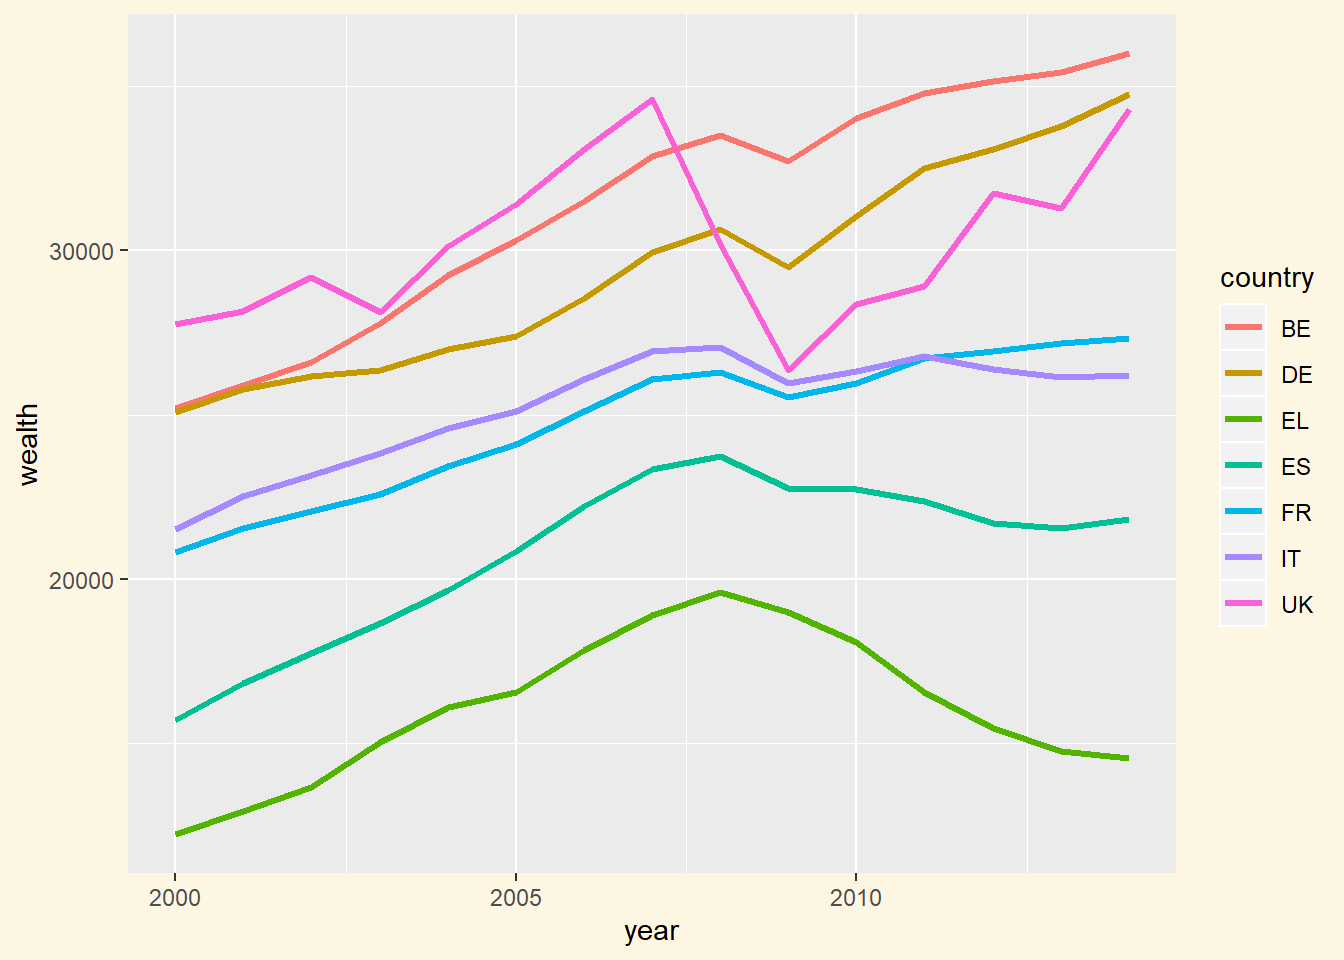
\includegraphics{r102_files/figure-latex/unnamed-chunk-72-1.pdf}

\hypertarget{merging-re-shaping-and-regular-expressions}{%
\section{Merging, re-shaping, and regular expressions}\label{merging-re-shaping-and-regular-expressions}}

\hypertarget{seminar-1}{%
\subsection{Seminar}\label{seminar-1}}

In this part of the course, we will merge data sets again. The difference to the previous exercise is that both data sets contain the same observations but different variables (columns) which is the more common case. We explain how re-shaping data works with a small ``toy'' example which should make the procedure more clear. Re-shaping is very often necessary for producing ggplot graphs. Finally, we will introduce a simple regular expression example. Regular expressions are extremely useful to identifying similar content that is not exactly identical.

\hypertarget{merging}{%
\subsubsection{Merging}\label{merging}}

We start by loading the \texttt{eu} data set again.

Download Data
Codebook

\begin{Shaded}
\begin{Highlighting}[]
\NormalTok{eu <-}\StringTok{ }\KeywordTok{read.csv}\NormalTok{(}\StringTok{"qog_eureg_long_sep16.csv"}\NormalTok{, }\DataTypeTok{stringsAsFactors =} \OtherTok{FALSE}\NormalTok{)}
\end{Highlighting}
\end{Shaded}

We now create a subset of the data set that only includes the variables \emph{year}, \emph{country}, \emph{region}, \emph{wealth}, \emph{quality.of.government}. We also filter by France, Germany, and the UK, and the years 2000 -- 2013. Furthermore, we must also filter out the observations within a country that are the country itself. Then, we save the data set as \texttt{eu\_subset1.csv}.

\begin{Shaded}
\begin{Highlighting}[]
\KeywordTok{library}\NormalTok{(tidyverse)}

\CommentTok{# copy, rename, select, filter, save}
\NormalTok{eu_subset12 <-}\StringTok{ }\NormalTok{eu }\OperatorTok
\StringTok{  }\NormalTok{dplyr}\OperatorTok{::}\KeywordTok{select}\NormalTok{(year,}
         \DataTypeTok{country =}\NormalTok{ NUTS0,}
         \DataTypeTok{region =}\NormalTok{ region_name,}
         \DataTypeTok{wealth =}\NormalTok{ econ_2gdp_eur_hab,}
         \DataTypeTok{quality.of.government =}\NormalTok{ eqi_eqi) }\OperatorTok
\StringTok{  }\KeywordTok{filter}\NormalTok{(country }\OperatorTok\StringTok{ }\KeywordTok{c}\NormalTok{(}\StringTok{"FR"}\NormalTok{, }\StringTok{"DE"}\NormalTok{, }\StringTok{"UK"}\NormalTok{) }\OperatorTok{&}\StringTok{ }\NormalTok{year }\OperatorTok{>}\StringTok{ }\DecValTok{1999} \OperatorTok{&}\StringTok{ }\NormalTok{year }\OperatorTok{<}\StringTok{ }\DecValTok{2014} \OperatorTok{&}\StringTok{ }
\StringTok{           }\OperatorTok{!}\NormalTok{(region }\OperatorTok\StringTok{ }\KeywordTok{c}\NormalTok{(}\StringTok{"DEUTSCHLAND "}\NormalTok{, }\StringTok{"FRANCE"}\NormalTok{, }\StringTok{"UNITED KINGDOM"}\NormalTok{))) }\OperatorTok
\StringTok{  }\KeywordTok{write.table}\NormalTok{(}\DataTypeTok{file =} \StringTok{"eu_subset1.csv"}\NormalTok{, }\DataTypeTok{sep =} \StringTok{","}\NormalTok{,}
              \DataTypeTok{row.names =} \OtherTok{FALSE}\NormalTok{, }\DataTypeTok{col.names =} \OtherTok{TRUE}\NormalTok{) }
\end{Highlighting}
\end{Shaded}

Let us create another subset of the original data set. It will include the same countries plus the Netherlands and Belgium but on the aggregate level, i.e.~it is not the regional level. Furthermore, there will be an additional variable which is the total population size but it will exclude wealth and the quality of government.

\begin{Shaded}
\begin{Highlighting}[]
\NormalTok{eu_subset2 <-}\StringTok{ }\NormalTok{eu }\OperatorTok
\StringTok{    }\NormalTok{dplyr}\OperatorTok{::}\KeywordTok{select}\NormalTok{(}
\NormalTok{      year,}
      \DataTypeTok{country =}\NormalTok{ NUTS0,}
      \DataTypeTok{population =}\NormalTok{ demo_d2jan_t) }\OperatorTok
\StringTok{  }\KeywordTok{filter}\NormalTok{(country }\OperatorTok\StringTok{ }\KeywordTok{c}\NormalTok{(}\StringTok{"FR"}\NormalTok{, }\StringTok{"DE"}\NormalTok{, }\StringTok{"UK"}\NormalTok{) }\OperatorTok{&}\StringTok{ }\NormalTok{year }\OperatorTok{>}\StringTok{ }\DecValTok{1999} \OperatorTok{&}\StringTok{ }\NormalTok{year }\OperatorTok{<}\StringTok{ }\DecValTok{2014}\NormalTok{) }\OperatorTok
\StringTok{  }\KeywordTok{group_by}\NormalTok{(country, year) }\OperatorTok
\StringTok{  }\KeywordTok{summarize}\NormalTok{(}\DataTypeTok{population =} \KeywordTok{sum}\NormalTok{(population, }\DataTypeTok{na.rm =} \OtherTok{TRUE}\NormalTok{)) }\OperatorTok
\StringTok{  }\KeywordTok{write.table}\NormalTok{(}\DataTypeTok{file =} \StringTok{"eu_subset2.csv"}\NormalTok{, }\DataTypeTok{sep =} \StringTok{","}\NormalTok{,}
              \DataTypeTok{row.names =} \OtherTok{FALSE}\NormalTok{, }\DataTypeTok{col.names =} \OtherTok{TRUE}\NormalTok{)}
\end{Highlighting}
\end{Shaded}

Note that we needed to use the \texttt{sum()} function in summarize rather than \texttt{mean()} when we wanted average wealth or average quality of government. The \emph{population} variable is the sum of the regional populations in a given year and country. To demonstrate merging, we now clear our workspace.

\begin{Shaded}
\begin{Highlighting}[]
\KeywordTok{rm}\NormalTok{(}\DataTypeTok{list=}\KeywordTok{ls}\NormalTok{())}
\end{Highlighting}
\end{Shaded}

We load the two data sets we created and inspect them. We do this to understand what will happen in merging.

\begin{Shaded}
\begin{Highlighting}[]
\NormalTok{eu1 <-}\StringTok{ }\KeywordTok{read.csv}\NormalTok{(}\DataTypeTok{file =} \StringTok{"eu_subset1.csv"}\NormalTok{, }\DataTypeTok{sep =} \StringTok{","}\NormalTok{, }\DataTypeTok{stringsAsFactors =} \OtherTok{FALSE}\NormalTok{)}
\NormalTok{eu2 <-}\StringTok{ }\KeywordTok{read.csv}\NormalTok{(}\DataTypeTok{file =} \StringTok{"eu_subset2.csv"}\NormalTok{, }\DataTypeTok{sep =} \StringTok{","}\NormalTok{, }\DataTypeTok{stringsAsFactors =} \OtherTok{FALSE}\NormalTok{)}
\end{Highlighting}
\end{Shaded}

We start by printing the first 30 observations of the \texttt{eu1} data set.

\begin{Shaded}
\begin{Highlighting}[]
\KeywordTok{head}\NormalTok{(eu1, }\DataTypeTok{n =} \DecValTok{30}\NormalTok{)}
\end{Highlighting}
\end{Shaded}

\begin{verbatim}
   year country             region wealth quality.of.government
1  2000      DE BADEN-WÃœRTTEMBERG  29700                    NA
2  2001      DE BADEN-WÃœRTTEMBERG  30900                    NA
3  2002      DE BADEN-WÃœRTTEMBERG  31000                    NA
4  2003      DE BADEN-WÃœRTTEMBERG  31100                    NA
5  2004      DE BADEN-WÃœRTTEMBERG  31400                    NA
6  2005      DE BADEN-WÃœRTTEMBERG  31700                    NA
7  2006      DE BADEN-WÃœRTTEMBERG  33700                    NA
8  2007      DE BADEN-WÃœRTTEMBERG  35600                    NA
9  2008      DE BADEN-WÃœRTTEMBERG  36000                    NA
10 2009      DE BADEN-WÃœRTTEMBERG  33600                    NA
11 2010      DE BADEN-WÃœRTTEMBERG  36400              1.010530
12 2011      DE BADEN-WÃœRTTEMBERG  38700                    NA
13 2012      DE BADEN-WÃœRTTEMBERG  39200                    NA
14 2013      DE BADEN-WÃœRTTEMBERG  39900              0.980281
15 2000      DE          Stuttgart  33300                    NA
16 2001      DE          Stuttgart  35000                    NA
17 2002      DE          Stuttgart  34800                    NA
18 2003      DE          Stuttgart  35200                    NA
19 2004      DE          Stuttgart  35200                    NA
20 2005      DE          Stuttgart  35100                    NA
21 2006      DE          Stuttgart  37700                    NA
22 2007      DE          Stuttgart  40200                    NA
23 2008      DE          Stuttgart  39800                    NA
24 2009      DE          Stuttgart  36600                    NA
25 2010      DE          Stuttgart  40500                    NA
26 2011      DE          Stuttgart  43000                    NA
27 2012      DE          Stuttgart  43900                    NA
28 2013      DE          Stuttgart  44700                    NA
29 2000      DE          Karlsruhe  29600                    NA
30 2001      DE          Karlsruhe  30600                    NA
\end{verbatim}

It is clear that the data set is on the region-year level. Let us inspect the second data set in the same way. We print the entire data set because it is much smaller.

\begin{Shaded}
\begin{Highlighting}[]
\NormalTok{eu2}
\end{Highlighting}
\end{Shaded}

\begin{verbatim}
   country year population
1       DE 2000  243755442
2       DE 2001  244065601
3       DE 2002  244632480
4       DE 2003  244944119
5       DE 2004  244947919
6       DE 2005  244873939
7       DE 2006  244702713
8       DE 2007  244352058
9       DE 2008  244080027
10      DE 2009  243452378
11      DE 2010  242869525
12      DE 2011  245254806
13      DE 2012  245531229
14      DE 2013  246061734
15      FR 2000  178261418
16      FR 2001  179512459
17      FR 2002  180795834
18      FR 2003  182067770
19      FR 2004  183303083
20      FR 2005  184699398
21      FR 2006  186029101
22      FR 2007  187235541
23      FR 2008  188276925
24      FR 2009  189281644
25      FR 2010  190189326
26      FR 2011  191119409
27      FR 2012  192028925
28      FR 2013  194898565
29      UK 2000  166803394
30      UK 2001  167366218
31      UK 2002  170368601
32      UK 2003  171117914
33      UK 2004  171966941
34      UK 2005  173069726
35      UK 2006  174302125
36      UK 2007  175573637
37      UK 2008  176961583
38      UK 2009  178249105
39      UK 2010  179527970
40      UK 2011  180934071
41      UK 2012  182228946
42      UK 2013  183352914
\end{verbatim}

This data set is on the country-year level. Let's say we want to merge the second data set to the first data set. The second data set includes the variable \emph{population} which will be added to the new combinded data set but the observations are one the country-year level. Therefore, all regions in a country-year will get the same population value (which is the population of the entire country). Because the second data set is more aggregated, we cannot get the population on a more dis-aggregated level but we can still combine both data sets. We do so with the \texttt{merge()} function

\begin{Shaded}
\begin{Highlighting}[]
\NormalTok{eu3 <-}\StringTok{ }\KeywordTok{merge}\NormalTok{(}\DataTypeTok{x =}\NormalTok{ eu1, }\DataTypeTok{y =}\NormalTok{ eu2, }\DataTypeTok{by =} \KeywordTok{c}\NormalTok{(}\StringTok{"year"}\NormalTok{, }\StringTok{"country"}\NormalTok{))}
\KeywordTok{dim}\NormalTok{(eu3)}
\end{Highlighting}
\end{Shaded}

\begin{verbatim}
[1] 2324    6
\end{verbatim}

So, the new data set has the same amount of observations as the bigger one but if we check the population variable, it is the same value for all regions within a country-year.

\hypertarget{re-shaping}{%
\subsubsection{Re-shaping}\label{re-shaping}}

Re-shaping a data set is useful, for instance for plotting graphs. For example, have a dependent variable, we an independent variable, and we have different model predictions. Let us create some a small data set with 10 observations and two correlated independent variables.

\begin{Shaded}
\begin{Highlighting}[]
\KeywordTok{library}\NormalTok{(MASS)}
\KeywordTok{set.seed}\NormalTok{(}\DecValTok{123}\NormalTok{)}

\CommentTok{# 2 correlated variables}
\NormalTok{X <-}\StringTok{ }\KeywordTok{mvrnorm}\NormalTok{(}\DataTypeTok{n =} \DecValTok{10}\NormalTok{, }\DataTypeTok{mu =} \KeywordTok{c}\NormalTok{(}\DecValTok{12}\NormalTok{, }\DecValTok{-4}\NormalTok{), }\DataTypeTok{Sigma =} \KeywordTok{matrix}\NormalTok{(}\DataTypeTok{data =} \KeywordTok{c}\NormalTok{(}\DecValTok{1}\NormalTok{, }\FloatTok{0.8}\NormalTok{, }\FloatTok{0.8}\NormalTok{, }\DecValTok{1}\NormalTok{), }\DataTypeTok{nrow =} \DecValTok{2}\NormalTok{, }\DataTypeTok{ncol =} \DecValTok{2}\NormalTok{))}
\NormalTok{X <-}\StringTok{ }\KeywordTok{data.frame}\NormalTok{(}\DataTypeTok{x1 =}\NormalTok{ X[,}\DecValTok{1}\NormalTok{], }\DataTypeTok{x2 =}\NormalTok{ X[,}\DecValTok{2}\NormalTok{])}
\NormalTok{X}
\end{Highlighting}
\end{Shaded}

\begin{verbatim}
         x1        x2
1  11.08120 -4.144625
2  11.66785 -4.104582
3  13.35199 -2.394544
4  12.03189 -3.898109
5  12.29843 -4.053119
6  13.06198 -1.807875
7  12.27983 -3.405302
8  11.42176 -5.822041
9  11.12661 -4.429818
10 11.72672 -4.572302
\end{verbatim}

Now that we have the two independent variables, let's create the outcome variable as a linear function of \emph{x2} and some random noise.

\begin{Shaded}
\begin{Highlighting}[]
\NormalTok{X}\OperatorTok{$}\NormalTok{y <-}\StringTok{ }\FloatTok{1.7} \OperatorTok{+}\StringTok{ }\NormalTok{X}\OperatorTok{$}\NormalTok{x2 }\OperatorTok{*}\StringTok{ }\FloatTok{-2.5} \OperatorTok{+}\StringTok{ }\KeywordTok{rnorm}\NormalTok{(}\DataTypeTok{n =} \DecValTok{10}\NormalTok{, }\DataTypeTok{mean =} \DecValTok{0}\NormalTok{, }\DataTypeTok{sd =} \DecValTok{3}\NormalTok{)}
\end{Highlighting}
\end{Shaded}

With this done, we run three linear models. The first includes \emph{x1} only, the second \emph{x2} only and the third both \emph{x1} and \emph{x2}. We then make prediction of y including confidence intervals for all three models and attach them to the data set.

\begin{Shaded}
\begin{Highlighting}[]
\CommentTok{# regressions}
\NormalTok{m1 <-}\StringTok{ }\KeywordTok{glm}\NormalTok{(y }\OperatorTok{~}\StringTok{ }\NormalTok{x1, }\DataTypeTok{family =} \StringTok{"gaussian"}\NormalTok{, }\DataTypeTok{data =}\NormalTok{ X)}
\NormalTok{m2 <-}\StringTok{ }\KeywordTok{glm}\NormalTok{(y }\OperatorTok{~}\StringTok{ }\NormalTok{x2, }\DataTypeTok{family =} \StringTok{"gaussian"}\NormalTok{, }\DataTypeTok{data =}\NormalTok{ X)}
\NormalTok{m3 <-}\StringTok{ }\KeywordTok{glm}\NormalTok{(y }\OperatorTok{~}\StringTok{ }\NormalTok{x1 }\OperatorTok{+}\StringTok{ }\NormalTok{x2, }\DataTypeTok{family =} \StringTok{"gaussian"}\NormalTok{, }\DataTypeTok{data =}\NormalTok{ X)}

\CommentTok{# predictions}
\NormalTok{preds1 <-}\StringTok{ }\KeywordTok{predict}\NormalTok{(m1, }\DataTypeTok{se.fit =} \OtherTok{TRUE}\NormalTok{)}
\NormalTok{preds2 <-}\StringTok{ }\KeywordTok{predict}\NormalTok{(m2, }\DataTypeTok{se.fit =} \OtherTok{TRUE}\NormalTok{)}
\NormalTok{preds3 <-}\StringTok{ }\KeywordTok{predict}\NormalTok{(m3, }\DataTypeTok{se.fit =} \OtherTok{TRUE}\NormalTok{)}

\CommentTok{# attach point estimates}
\NormalTok{X}\OperatorTok{$}\NormalTok{bestguess1 <-}\StringTok{ }\NormalTok{preds1}\OperatorTok{$}\NormalTok{fit}
\NormalTok{X}\OperatorTok{$}\NormalTok{bestguess2 <-}\StringTok{ }\NormalTok{preds2}\OperatorTok{$}\NormalTok{fit}
\NormalTok{X}\OperatorTok{$}\NormalTok{bestguess3 <-}\StringTok{ }\NormalTok{preds3}\OperatorTok{$}\NormalTok{fit}

\CommentTok{# attach lower and upper bounds of the 95% CI from a t with the appropriate degrees of freedom}
\NormalTok{X}\OperatorTok{$}\NormalTok{lowerbound1 <-}\StringTok{ }\NormalTok{preds1}\OperatorTok{$}\NormalTok{fit }\OperatorTok{-}\StringTok{ }\KeywordTok{qt}\NormalTok{(}\DataTypeTok{p =} \FloatTok{0.975}\NormalTok{, }\DataTypeTok{df =}\NormalTok{ m1}\OperatorTok{$}\NormalTok{df.residual) }\OperatorTok{*}\StringTok{ }\NormalTok{preds1}\OperatorTok{$}\NormalTok{se.fit}
\NormalTok{X}\OperatorTok{$}\NormalTok{lowerbound2 <-}\StringTok{ }\NormalTok{preds2}\OperatorTok{$}\NormalTok{fit }\OperatorTok{-}\StringTok{ }\KeywordTok{qt}\NormalTok{(}\DataTypeTok{p =} \FloatTok{0.975}\NormalTok{, }\DataTypeTok{df =}\NormalTok{ m2}\OperatorTok{$}\NormalTok{df.residual) }\OperatorTok{*}\StringTok{ }\NormalTok{preds2}\OperatorTok{$}\NormalTok{se.fit}
\NormalTok{X}\OperatorTok{$}\NormalTok{lowerbound3 <-}\StringTok{ }\NormalTok{preds3}\OperatorTok{$}\NormalTok{fit }\OperatorTok{-}\StringTok{ }\KeywordTok{qt}\NormalTok{(}\DataTypeTok{p =} \FloatTok{0.975}\NormalTok{, }\DataTypeTok{df =}\NormalTok{ m3}\OperatorTok{$}\NormalTok{df.residual) }\OperatorTok{*}\StringTok{ }\NormalTok{preds3}\OperatorTok{$}\NormalTok{se.fit}
\NormalTok{X}\OperatorTok{$}\NormalTok{upperbound1 <-}\StringTok{ }\NormalTok{preds1}\OperatorTok{$}\NormalTok{fit }\OperatorTok{+}\StringTok{ }\KeywordTok{qt}\NormalTok{(}\DataTypeTok{p =} \FloatTok{0.975}\NormalTok{, }\DataTypeTok{df =}\NormalTok{ m1}\OperatorTok{$}\NormalTok{df.residual) }\OperatorTok{*}\StringTok{ }\NormalTok{preds1}\OperatorTok{$}\NormalTok{se.fit}
\NormalTok{X}\OperatorTok{$}\NormalTok{upperbound2 <-}\StringTok{ }\NormalTok{preds2}\OperatorTok{$}\NormalTok{fit }\OperatorTok{+}\StringTok{ }\KeywordTok{qt}\NormalTok{(}\DataTypeTok{p =} \FloatTok{0.975}\NormalTok{, }\DataTypeTok{df =}\NormalTok{ m2}\OperatorTok{$}\NormalTok{df.residual) }\OperatorTok{*}\StringTok{ }\NormalTok{preds2}\OperatorTok{$}\NormalTok{se.fit}
\NormalTok{X}\OperatorTok{$}\NormalTok{upperbound3 <-}\StringTok{ }\NormalTok{preds3}\OperatorTok{$}\NormalTok{fit }\OperatorTok{+}\StringTok{ }\KeywordTok{qt}\NormalTok{(}\DataTypeTok{p =} \FloatTok{0.975}\NormalTok{, }\DataTypeTok{df =}\NormalTok{ m3}\OperatorTok{$}\NormalTok{df.residual) }\OperatorTok{*}\StringTok{ }\NormalTok{preds3}\OperatorTok{$}\NormalTok{se.fit}

\CommentTok{# print data set}
\NormalTok{X}
\end{Highlighting}
\end{Shaded}

\begin{verbatim}
         x1        x2         y bestguess1 bestguess2 bestguess3
1  11.08120 -4.144625  8.858092  13.699237  11.130489   9.641748
2  11.66785 -4.104582 11.307531  11.403226  10.981629  10.589413
3  13.35199 -2.394544  4.608348   4.811964   4.624524   5.644261
4  12.03189 -3.898109  9.258599   9.978477  10.214059  10.304613
5  12.29843 -4.053119  9.957680   8.935323  10.790314  11.567548
6  13.06198 -1.807875  1.159607   5.946962   2.443567   2.261255
7  12.27983 -3.405302 12.726617   9.008104   8.382040   8.418132
8  11.42176 -5.822041 16.715223  12.366378  17.366322  18.364911
9  11.12661 -4.429818  9.360133  13.521520  12.190699  11.100571
10 11.72672 -4.572302 16.892199  11.172839  12.720387  12.951578
   lowerbound1 lowerbound2 lowerbound3 upperbound1 upperbound2 upperbound3
1    8.9231907    9.185198    5.493225    18.47528   13.075781    13.79027
2    8.1521159    9.053073    8.385503    14.65434   12.910186    12.79332
3   -1.4113612    1.427737    1.518502    11.03529    7.821311     9.77002
4    7.0285045    8.331855    8.354573    12.92845   12.096264    12.25465
5    5.7545940    8.879660    8.835127    12.11605   12.700968    14.29997
6    0.7326925   -1.633502   -1.959061    11.16123    6.520636     6.48157
7    5.8550072    6.335486    6.309639    12.16120   10.428593    10.52662
8    8.5825423   13.439212   13.644692    16.15021   21.293433    23.08513
9    8.8894214   10.061580    7.653651    18.15362   14.319817    14.54749
10   8.0152435   10.462938   10.560320    14.33043   14.977835    15.34284
\end{verbatim}

The data set is in the common format for analysis. However, if we want to plot the predictions in ggplot and differentiate them with color by model, we have to re-shape the data set into a long format. In long format, we want to have a new variable called \emph{model} which takes on the values ``model 1'', ``model 2'', ``model 3'' corresponding to the respective model that made the prediction of a best guess, lower or upper bound. We make the data set three times as long by combining \emph{bestguess1}, \emph{bestguess2}, and \emph{bestguess3} into one \emph{bestguess} variable. We do the same with the upper and lower bounds. The variables \emph{x1}, \emph{x2}, and \emph{y} are so called ``id'' variables because we just recycle the values that are already there, i.e.~nothing is combined here. We use the \texttt{reshape()} function.

Have a look at the argument's meaning in the help window (usually at lower right in RStudio) by running \texttt{?reshape}.

\begin{Shaded}
\begin{Highlighting}[]
\NormalTok{eu.long <-}\StringTok{ }\KeywordTok{reshape}\NormalTok{(}\DataTypeTok{data =}\NormalTok{ X, }\DataTypeTok{varying =} \KeywordTok{c}\NormalTok{(}\StringTok{"bestguess1"}\NormalTok{, }\StringTok{"lowerbound1"}\NormalTok{, }\StringTok{"upperbound1"}\NormalTok{,}
                                         \StringTok{"bestguess2"}\NormalTok{, }\StringTok{"lowerbound2"}\NormalTok{, }\StringTok{"upperbound2"}\NormalTok{,}
                                         \StringTok{"bestguess3"}\NormalTok{, }\StringTok{"lowerbound3"}\NormalTok{, }\StringTok{"upperbound3"}\NormalTok{),}
                   \DataTypeTok{timevar =} \StringTok{"Model"}\NormalTok{,}
                   \DataTypeTok{times =} \KeywordTok{c}\NormalTok{(}\DecValTok{1}\NormalTok{,}\DecValTok{2}\NormalTok{,}\DecValTok{3}\NormalTok{),}
                   \DataTypeTok{v.names =} \KeywordTok{c}\NormalTok{(}\StringTok{"bestguess"}\NormalTok{,}\StringTok{"lowerbound"}\NormalTok{,}\StringTok{"upperbound"}\NormalTok{),}
                   \DataTypeTok{idvar =} \KeywordTok{c}\NormalTok{(}\StringTok{"x1"}\NormalTok{,}\StringTok{"x2"}\NormalTok{, }\StringTok{"y"}\NormalTok{),}
                   \DataTypeTok{direction =} \StringTok{"long"}\NormalTok{)}

\CommentTok{# change the row.names which are always combinations of the idvars}
\KeywordTok{row.names}\NormalTok{(eu.long) <-}\StringTok{ }\KeywordTok{seq}\NormalTok{(}\DecValTok{1}\OperatorTok{:}\KeywordTok{nrow}\NormalTok{(eu.long))}

\CommentTok{# inspect data set}
\NormalTok{eu.long}
\end{Highlighting}
\end{Shaded}

\begin{verbatim}
         x1        x2         y Model bestguess lowerbound upperbound
1  11.08120 -4.144625  8.858092     1 13.699237  8.9231907  18.475283
2  11.66785 -4.104582 11.307531     1 11.403226  8.1521159  14.654337
3  13.35199 -2.394544  4.608348     1  4.811964 -1.4113612  11.035289
4  12.03189 -3.898109  9.258599     1  9.978477  7.0285045  12.928450
5  12.29843 -4.053119  9.957680     1  8.935323  5.7545940  12.116053
6  13.06198 -1.807875  1.159607     1  5.946962  0.7326925  11.161232
7  12.27983 -3.405302 12.726617     1  9.008104  5.8550072  12.161200
8  11.42176 -5.822041 16.715223     1 12.366378  8.5825423  16.150213
9  11.12661 -4.429818  9.360133     1 13.521520  8.8894214  18.153618
10 11.72672 -4.572302 16.892199     1 11.172839  8.0152435  14.330434
11 11.08120 -4.144625  8.858092     2 11.130489  9.1851978  13.075781
12 11.66785 -4.104582 11.307531     2 10.981629  9.0530726  12.910186
13 13.35199 -2.394544  4.608348     2  4.624524  1.4277367   7.821311
14 12.03189 -3.898109  9.258599     2 10.214059  8.3318549  12.096264
15 12.29843 -4.053119  9.957680     2 10.790314  8.8796601  12.700968
16 13.06198 -1.807875  1.159607     2  2.443567 -1.6335023   6.520636
17 12.27983 -3.405302 12.726617     2  8.382040  6.3354862  10.428593
18 11.42176 -5.822041 16.715223     2 17.366322 13.4392116  21.293433
19 11.12661 -4.429818  9.360133     2 12.190699 10.0615797  14.319817
20 11.72672 -4.572302 16.892199     2 12.720387 10.4629384  14.977835
21 11.08120 -4.144625  8.858092     3  9.641748  5.4932253  13.790271
22 11.66785 -4.104582 11.307531     3 10.589413  8.3855035  12.793322
23 13.35199 -2.394544  4.608348     3  5.644261  1.5185017   9.770020
24 12.03189 -3.898109  9.258599     3 10.304613  8.3545732  12.254654
25 12.29843 -4.053119  9.957680     3 11.567548  8.8351269  14.299969
26 13.06198 -1.807875  1.159607     3  2.261255 -1.9590606   6.481570
27 12.27983 -3.405302 12.726617     3  8.418132  6.3096388  10.526625
28 11.42176 -5.822041 16.715223     3 18.364911 13.6446922  23.085130
29 11.12661 -4.429818  9.360133     3 11.100571  7.6536509  14.547492
30 11.72672 -4.572302 16.892199     3 12.951578 10.5603200  15.342836
\end{verbatim}

Ee turn the variable model into a factor variable.

\begin{Shaded}
\begin{Highlighting}[]
\NormalTok{eu.long}\OperatorTok{$}\NormalTok{Model <-}\StringTok{ }\KeywordTok{factor}\NormalTok{(eu.long}\OperatorTok{$}\NormalTok{Model, }\DataTypeTok{levels =} \KeywordTok{c}\NormalTok{(}\DecValTok{1}\NormalTok{,}\DecValTok{2}\NormalTok{,}\DecValTok{3}\NormalTok{), }\DataTypeTok{labels =} \KeywordTok{c}\NormalTok{(}\StringTok{"Incorrect Model"}\NormalTok{, }\StringTok{"Correct Model"}\NormalTok{, }\StringTok{"Full Model"}\NormalTok{))}
\KeywordTok{table}\NormalTok{(eu.long}\OperatorTok{$}\NormalTok{Model)}
\end{Highlighting}
\end{Shaded}

\begin{verbatim}

Incorrect Model   Correct Model      Full Model 
             10              10              10 
\end{verbatim}

We plot using ggplot.

\begin{Shaded}
\begin{Highlighting}[]
\KeywordTok{ggplot}\NormalTok{(eu.long, }\KeywordTok{aes}\NormalTok{(}\DataTypeTok{x =}\NormalTok{ x2, }\DataTypeTok{y =}\NormalTok{ y)) }\OperatorTok{+}
\StringTok{  }\KeywordTok{geom_point}\NormalTok{() }\OperatorTok{+}
\StringTok{  }\KeywordTok{geom_line}\NormalTok{( }\KeywordTok{aes}\NormalTok{(}\DataTypeTok{y =}\NormalTok{ bestguess, }\DataTypeTok{color =}\NormalTok{ Model)) }\OperatorTok{+}
\StringTok{  }\KeywordTok{geom_ribbon}\NormalTok{( }\KeywordTok{aes}\NormalTok{(}\DataTypeTok{ymin =}\NormalTok{ lowerbound, }\DataTypeTok{ymax =}\NormalTok{ upperbound, }\DataTypeTok{fill =}\NormalTok{ Model), }\DataTypeTok{alpha =} \FloatTok{0.3}\NormalTok{)}
\end{Highlighting}
\end{Shaded}

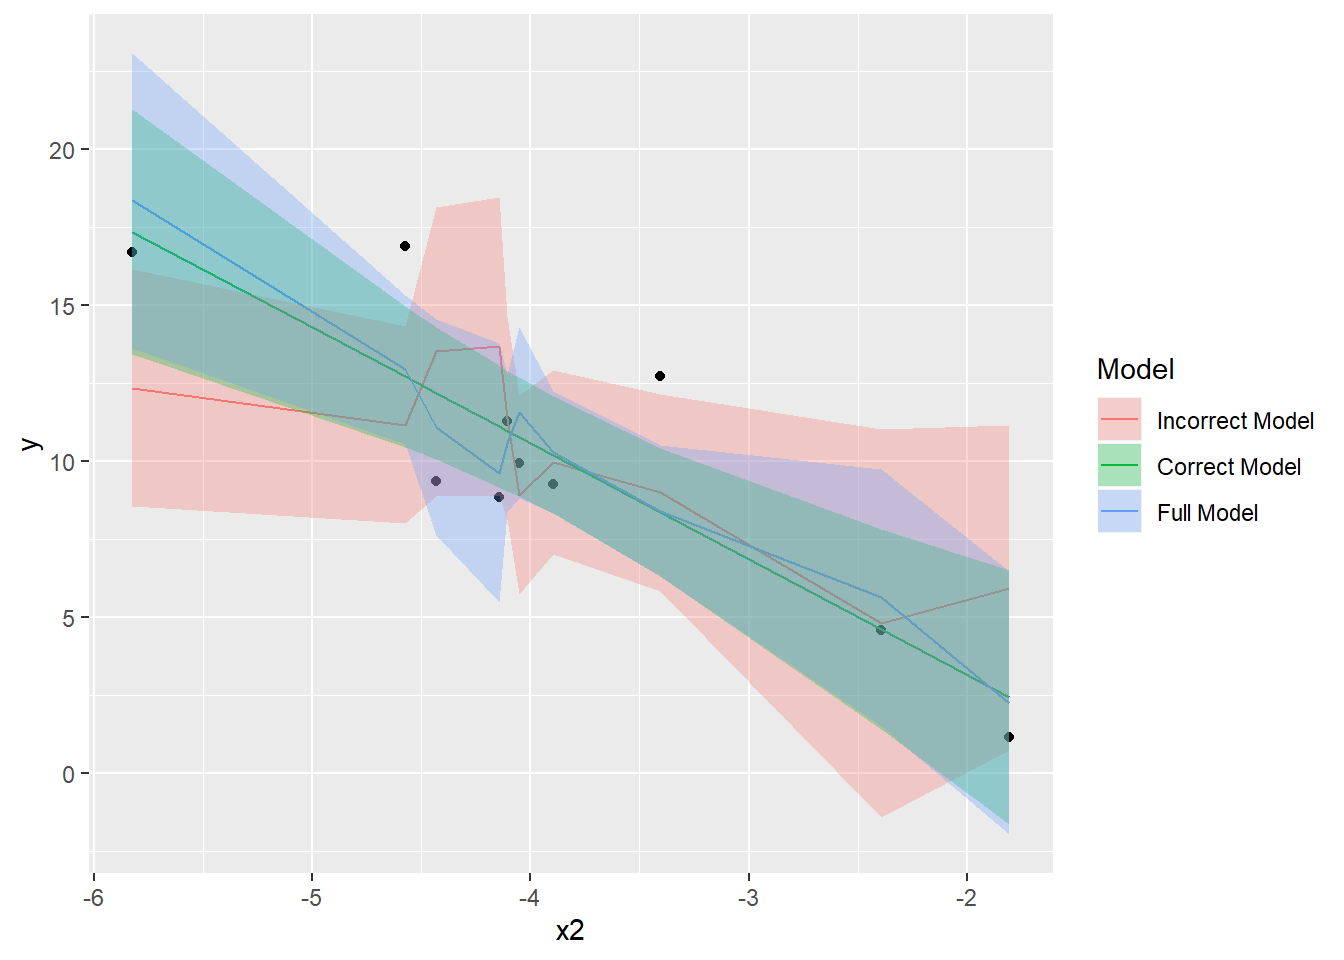
\includegraphics{r102_files/figure-latex/unnamed-chunk-88-1.pdf}

We see that the all model predictions overlap. The incorrect model does worst and also has the largest amount of uncertainty. While it is hard to see, the correct model is closest to the real predictions and has the smallest uncertainty. Go ahead and plot the size of the residuals on your own.

\hypertarget{regular-expression}{%
\subsubsection{Regular expression}\label{regular-expression}}

Regular expressions are difficult to master but very powerful when it comes to working with data. Regular expressions can be used to extract email addresses, phone numbers, country names and much more. We provide a simple example and invite you to search online for more complex tasks.

We examine the \texttt{eu} data set and the regions in the UK.

\begin{Shaded}
\begin{Highlighting}[]
\KeywordTok{unique}\NormalTok{(eu1}\OperatorTok{$}\NormalTok{region[eu1}\OperatorTok{$}\NormalTok{country}\OperatorTok{==}\StringTok{"UK"}\NormalTok{])}
\end{Highlighting}
\end{Shaded}

\begin{verbatim}
 [1] "NORTH EAST (ENGLAND)"                            
 [2] "Tees Valley and Durham"                          
 [3] "Northumberland and Tyne and Wear"                
 [4] "NORTH WEST (ENGLAND)"                            
 [5] "Cumbria"                                         
 [6] "Cheshire"                                        
 [7] "Greater Manchester"                              
 [8] "Lancashire"                                      
 [9] "Merseyside"                                      
[10] "YORKSHIRE AND THE HUMBER"                        
[11] "East Yorkshire and Northern Lincolnshire"        
[12] "North Yorkshire"                                 
[13] "South Yorkshire"                                 
[14] "West Yorkshire"                                  
[15] "EAST MIDLANDS (ENGLAND)"                         
[16] "Derbyshire and Nottinghamshire"                  
[17] "Leicestershire, Rutland and Northamptonshire"    
[18] "Lincolnshire"                                    
[19] "WEST MIDLANDS (ENGLAND)"                         
[20] "Herefordshire, Worcestershire and Warwickshire"  
[21] "Shropshire and Staffordshire"                    
[22] "West Midlands"                                   
[23] "EAST OF ENGLAND"                                 
[24] "East Anglia"                                     
[25] "Bedfordshire and Hertfordshire"                  
[26] "Essex"                                           
[27] "LONDON"                                          
[28] "Inner London"                                    
[29] "Outer London"                                    
[30] "Inner London - West"                             
[31] "Inner London - East"                             
[32] "Outer London - East and North East"              
[33] "Outer London - South"                            
[34] "Outer London - West and North West"              
[35] "SOUTH EAST (ENGLAND)"                            
[36] "Berkshire, Buckinghamshire and Oxfordshire"      
[37] "Surrey, East and West Sussex"                    
[38] "Hampshire and Isle of Wight"                     
[39] "Kent"                                            
[40] "SOUTH WEST (ENGLAND)"                            
[41] "Gloucestershire, Wiltshire and Bristol/Bath area"
[42] "Dorset and Somerset"                             
[43] "Cornwall and Isles of Scilly"                    
[44] "Devon"                                           
[45] "WALES"                                           
[46] "West Wales and The Valleys"                      
[47] "East Wales"                                      
[48] "SCOTLAND"                                        
[49] "North Eastern Scotland"                          
[50] "Eastern Scotland"                                
[51] "South Western Scotland"                          
[52] "Highlands and Islands"                           
[53] "NORTHERN IRELAND"                                
[54] "Northern Ireland"                                
[55] "EXTRA-REGIO NUTS 1"                              
[56] "Extra-Regio NUTS 2"                              
\end{verbatim}

There are multiple regions of London in the data set. Say we wanted to aggregate wealth for all the London regions but we did not want to pick out the regions by hand. This is what regular expressions excel at. We use the \texttt{grep()} function which returns the row numbers of all London districts. Let's subset the data set to London only and then compare the wealth of London regions over time in a plot.

\begin{Shaded}
\begin{Highlighting}[]
\KeywordTok{grep}\NormalTok{(}\DataTypeTok{pattern =} \StringTok{"London"}\NormalTok{, }\DataTypeTok{x =}\NormalTok{ eu1}\OperatorTok{$}\NormalTok{region, }\DataTypeTok{ignore.case =} \OtherTok{TRUE}\NormalTok{)}
\end{Highlighting}
\end{Shaded}

\begin{verbatim}
  [1] 1877 1878 1879 1880 1881 1882 1883 1884 1885 1886 1887 1888 1889 1890
 [15] 1891 1892 1893 1894 1895 1896 1897 1898 1899 1900 1901 1902 1903 1904
 [29] 1905 1906 1907 1908 1909 1910 1911 1912 1913 1914 1915 1916 1917 1918
 [43] 1919 1920 1921 1922 1923 1924 1925 1926 1927 1928 1929 1930 1931 1932
 [57] 1933 1934 1935 1936 1937 1938 1939 1940 1941 1942 1943 1944 1945 1946
 [71] 1947 1948 1949 1950 1951 1952 1953 1954 1955 1956 1957 1958 1959 1960
 [85] 1961 1962 1963 1964 1965 1966 1967 1968 1969 1970 1971 1972 1973 1974
 [99] 1975 1976 1977 1978 1979 1980 1981 1982 1983 1984 1985 1986 1987 1988
\end{verbatim}

\begin{Shaded}
\begin{Highlighting}[]
\NormalTok{london <-}\StringTok{ }\NormalTok{eu1 }\OperatorTok
\StringTok{  }\KeywordTok{slice}\NormalTok{( }\KeywordTok{grep}\NormalTok{(}\DataTypeTok{pattern =} \StringTok{"London"}\NormalTok{, }\DataTypeTok{x =}\NormalTok{ eu1}\OperatorTok{$}\NormalTok{region, }\DataTypeTok{ignore.case =} \OtherTok{TRUE}\NormalTok{) ) }\OperatorTok
\StringTok{  }\KeywordTok{filter}\NormalTok{( region }\OperatorTok{!=}\StringTok{ "LONDON"}\NormalTok{ )}

\KeywordTok{ggplot}\NormalTok{(london, }\KeywordTok{aes}\NormalTok{(}\DataTypeTok{x =}\NormalTok{ year, }\DataTypeTok{y =}\NormalTok{ wealth)) }\OperatorTok{+}
\StringTok{       }\KeywordTok{geom_line}\NormalTok{( }\KeywordTok{aes}\NormalTok{(}\DataTypeTok{y =}\NormalTok{ wealth, }\DataTypeTok{color =}\NormalTok{ region)) }
\end{Highlighting}
\end{Shaded}

\begin{verbatim}
Warning: Removed 28 rows containing missing values (geom_path).
\end{verbatim}

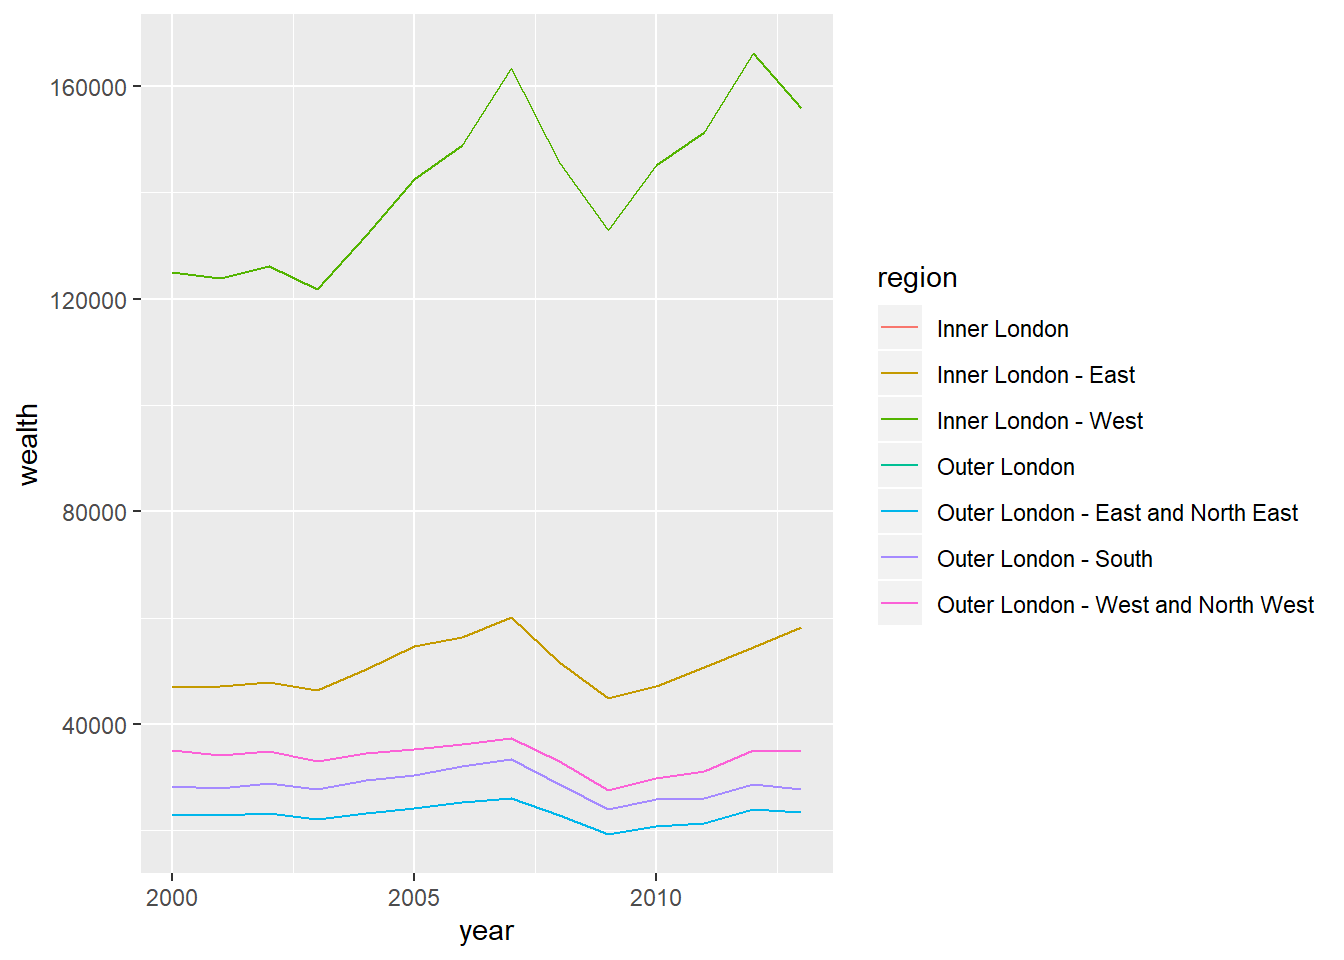
\includegraphics{r102_files/figure-latex/unnamed-chunk-91-1.pdf}

It seems like Inner London - West is the place to be.


\end{document}
